% fc3_approximations.tex
%
% Replaces/extends the content of main-doc.tex from
%   \subsection{Reduced FC3 models for transport}
% through the end of the anharmonic section.
%
% For standalone compilation, uncomment the preamble below.
% For inclusion in main-doc.tex, comment out the preamble and
% \begin/\end{document}, and use % fc3_approximations.tex
%
% Replaces/extends the content of main-doc.tex from
%   \subsection{Reduced FC3 models for transport}
% through the end of the anharmonic section.
%
% For standalone compilation, uncomment the preamble below.
% For inclusion in main-doc.tex, comment out the preamble and
% \begin/\end{document}, and use % fc3_approximations.tex
%
% Replaces/extends the content of main-doc.tex from
%   \subsection{Reduced FC3 models for transport}
% through the end of the anharmonic section.
%
% For standalone compilation, uncomment the preamble below.
% For inclusion in main-doc.tex, comment out the preamble and
% \begin/\end{document}, and use % fc3_approximations.tex
%
% Replaces/extends the content of main-doc.tex from
%   \subsection{Reduced FC3 models for transport}
% through the end of the anharmonic section.
%
% For standalone compilation, uncomment the preamble below.
% For inclusion in main-doc.tex, comment out the preamble and
% \begin/\end{document}, and use \input{anharmonic/fc3_approximations}.
%
\documentclass[11pt]{article}
\usepackage[margin=2.5cm]{geometry}
\usepackage{amsmath, amssymb, bm}
\usepackage{booktabs}
\usepackage{graphicx}
\usepackage{siunitx}
\usepackage{hyperref}
\usepackage{cleveref}
\usepackage{xcolor}

% Macros (must match main-doc.tex when included there)
\newcommand{\vc}[1]{\bm{#1}}
\newcommand{\ndof}{n_{\mathrm{dof}}}
\newcommand{\nprim}{n_{\mathrm{prim}}}
\newcommand{\nsuper}{n_{\mathrm{super}}}
\DeclareMathOperator{\diag}{diag}
\DeclareMathOperator{\tr}{tr}
\DeclareMathOperator{\vect}{vec}

\newcommand{\vq}{\vc{q}}
\newcommand{\vR}{\vc{R}}
\newcommand{\va}{\vc{a}}
\newcommand{\vrho}{\bm{\rho}}
\newcommand{\PhiT}{\tilde{\Phi}}
\newcommand{\Sig}{\Sigma}
\newcommand{\sS}{\mathcal{S}}
\newcommand{\cO}{\mathcal{O}}
\newcommand{\cC}{\mathcal{C}}
\newcommand{\cW}{\mathcal{W}}
\newcommand{\dw}{\frac{d\omega'}{2\pi}}

\graphicspath{{figures/}}

\title{Low-Rank FC3 Approximations and\\
       Anharmonic Phonon Transport}
\author{}
\date{}

\begin{document}
\maketitle
\tableofcontents
\newpage

%#######################################################################
%
%  PART I — THEORY
%
%#######################################################################

% ======================================================================
\section{FC3 tensor and transport}
\label{sec:fc3_tensor}
% ======================================================================

% ----------------------------------------------------------------------
\subsection{The compact FC3 tensor}
\label{sec:compact_fc3}
% ----------------------------------------------------------------------

The third-order force constant (FC3) tensor, obtained from a supercell
finite-displacement or DFPT calculation, is
\begin{equation}\label{eq:fc3}
  \Phi_{\alpha\beta\gamma}(0\kappa,\; l'\kappa',\; l''\kappa'')
  = \frac{\partial^3 E}
         {\partial u_\alpha(0\kappa)\,
          \partial u_\beta(l'\kappa')\,
          \partial u_\gamma(l''\kappa'')}\,.
\end{equation}
In the compact format, the first atom index is restricted to the
primitive cell (cell~0), while the remaining two run over the full
$N_1\!\times\!N_2\!\times\!N_3$ supercell.  After mass-weighting, the
composite DOF labels are
\begin{equation}
  a = (\kappa, \alpha), \qquad
  c = (l'\kappa', \beta), \qquad
  d = (l''\kappa'', \gamma),
\end{equation}
so the target tensor is
\begin{equation}\label{eq:target}
  \Phi_{acd}\,, \qquad
  a \in \{1,\dots,\ndof\}, \quad
  c, d \in \{1,\dots,D\},
\end{equation}
with $\ndof = 3\,\nprim$ and $D = 3\,\nsuper$.  The exchange symmetry
$\Phi_{acd} = \Phi_{adc}$ holds for the internal indices.

The full tensor has $\ndof \times D^2$ entries.  For silicon
($\nprim = 2$, $\ndof = 6$) in a $2\times2\times2$ supercell
($\nsuper = 16$, $D = 48$): $13\,824$ entries; in a
$3\times3\times3$ supercell ($\nsuper = 54$, $D = 162$):
$157\,464$ entries.

% ----------------------------------------------------------------------
\subsection{Reduced FC3 models for transport}
\label{sec:assembly_fc3}
% ----------------------------------------------------------------------

In the transport implementation, the harmonic device region is one
transport cell thick, with harmonic dimension $\ndof = 3N_b$ where
$N_b$ is the number of basis atoms.  The full FC3 couples triplets
across different unit cells, exceeding the locality of the single-slab
representation.

\subsubsection{Onsite approximation}

The simplest reduction retains only the fully local FC3 block:
\begin{equation}
  \Psi_{abc}^{\mathrm{onsite}}
  = \frac{\Phi^{(3)}_{abc}(\vc{0},\vc{0},\vc{0})}
         {\sqrt{M_a M_b M_c}}\,.
\end{equation}
This ignores all cubic couplings to neighbouring slabs.

\subsubsection{Full $\delta l = 0$ approximation}

A less restrictive approximation retains all FC3 blocks whose relative
cell vectors remain within the same transport slab:
\begin{equation}\label{eq:fc3_full}
  \Psi_{abc}^{\mathrm{full}}
  = \sum_{\substack{\vR',\vR'' \\
                    \delta l' = 0,\;\delta l'' = 0}}
  \frac{\Phi^{(3)}_{abc}(\vc{0},\vR',\vR'')}
       {\sqrt{M_a M_b M_c}}\,.
\end{equation}

\subsubsection{Low-rank approximations}

Both onsite and $\delta l = 0$ approximations are spatial truncations
that discard coupling between transport slabs.  A fundamentally
different approach is to compress the full FC3 tensor algebraically,
retaining all spatial couplings but representing the tensor with fewer
parameters.  This is the subject of
\cref{sec:svd,sec:pscp,sec:scp3,sec:fscp}.


% ======================================================================
\section{Phonon--phonon self-energy}
\label{sec:self_energy}
% ======================================================================

% ----------------------------------------------------------------------
\subsection{Self-energy formula}
\label{sec:se_formula}
% ----------------------------------------------------------------------

The lowest-order phonon--phonon scattering self-energy connects two FC3
vertices with two Green's functions.  The lesser component is
\begin{equation}\label{eq:sigma_guo}
  \Sigma^{<}_{ab}(\omega)
  = \frac{i\hbar}{2}
    \sum_{c,d,e,f}
    \Psi_{acd}
    \left[
      \int \frac{d\omega'}{2\pi}\;
      G^<_{ce}(\omega')\,
      G^<_{df}(\omega-\omega')
    \right]
    \Psi_{bef}\,,
\end{equation}
with analogous expressions for $\Sigma^{>}$ and the retarded
approximation
\begin{equation}\label{eq:sigma_r}
  \Sigma^R(\omega) \approx \tfrac{1}{2}
  \bigl[\Sigma^>(\omega) - \Sigma^<(\omega)\bigr].
\end{equation}

% ----------------------------------------------------------------------
\subsection{Full Fourier-space self-energy}
\label{sec:fourier_se}
% ----------------------------------------------------------------------

For a system with transverse periodicity, the self-energy depends on
the transverse wavevector and includes an internal momentum sum:
\begin{align}\label{eq:sigma_phph}
  \Sigma^{\gtrless}_{s,\,ll'_s}(&\omega;\,\vq_\perp)
  = \frac{i\hbar}{2}
    \sum_{\substack{l_1 l_2 l_3 l_4\\ j_1 j_2 j_3 j_4}}
    \frac{1}{N}\sum_{\vq'_\perp}
    \PhiT^{ij_1j_2}_{l,\,l_1 l_2}
      \!\left(\vq'_\perp,\vq_\perp\!-\!\vq'_\perp\right)
    \notag\\
  &\qquad\times
    \PhiT^{j_3j_4j}_{l',\,l_3 l_4}
      \!\left(\vq'_\perp\!-\!\vq_\perp,-\vq'_\perp\right)
    \int\!\dw\;
    G^{\gtrless,j_1j_4}_{l_1l_4}(\omega';\vq'_\perp)\,
    G^{\gtrless,j_2j_3}_{l_2l_3}
      (\omega\!-\!\omega';\vq_\perp\!-\!\vq'_\perp).
\end{align}
The Fourier-transformed FC3 depends on \emph{two} wavevectors:
\begin{equation}\label{eq:fc3_fourier}
  \PhiT^{ij_1j_2}_{l,l_{1}l_{2}}(\vq,\vq')
  = \sum_{\vrho_1}\sum_{\vrho_2}
  \Phi^{ij_1j_2}_{l,l_1,l_2}\;
  e^{-i\vq\cdot\vrho_1}\;e^{-i\vq'\cdot\vrho_2}.
\end{equation}
Unlike the harmonic problem where each $\vq_\perp$ is independent, the
internal $\vq'_\perp$ sum couples all transverse wavevectors.  This is
the origin of the substantially greater computational complexity of the
anharmonic problem.

% ----------------------------------------------------------------------
\subsection{Frequency discretisation and FFT convolution}
\label{sec:fft}
% ----------------------------------------------------------------------

The frequency integral in \cref{eq:sigma_guo} is a convolution,
evaluated on a discrete grid
$\omega_n = \omega_\mathrm{min} + n\,\Delta\omega$ by FFT:
\begin{equation}
  C_{ce,df}[\omega_n]
  = \frac{\Delta\omega}{2\pi}
    \sum_m
    G^<_{ce}[\omega_m]\;G^<_{df}[\omega_n - \omega_m]
  = \frac{\Delta\omega}{2\pi}\,
    \mathrm{IFFT}\!\bigl[
      \mathrm{FFT}(G_{ce})\cdot \mathrm{FFT}(G_{df})
    \bigr].
\end{equation}
The broadening parameter is $\eta = \eta_\mathrm{factor}\,(\Delta\omega)^2$
with $\eta_\mathrm{factor} = 0.5$.


% ======================================================================
\section{SCBA algorithm}
\label{sec:scba}
% ======================================================================

The phonon self-energy modifies the Green's functions, which in turn
modify the self-energy.  This nonlinear problem is solved iteratively
within the self-consistent Born approximation (SCBA).

% ----------------------------------------------------------------------
\subsection{SCBA loop}
\label{sec:scba_loop}
% ----------------------------------------------------------------------

\begin{enumerate}
  \item \textbf{Initialization.}
        $\Sigma^\mathrm{ph} = 0$; solve the ballistic transport problem.

  \item \textbf{Green's functions.}
        For each $(\vq_\perp, \omega_n)$:
        \begin{align}
          G^R &= \bigl[(\omega^2+i\eta)\,\mathbb{I}
                 - H_{00} - \Sigma_L^R - \Sigma_R^R
                 - \Sigma_\mathrm{ph}^R\bigr]^{-1}, \\
          G^{<,>} &= G^R\,\Sigma^{<,>}_\mathrm{total}\,(G^R)^\dagger.
        \end{align}

  \item \textbf{Self-energy update.}
        Construct the new $\Sigma_\mathrm{ph}^{<,>,R}$ from
        \cref{eq:sigma_guo,eq:sigma_r}.

  \item \textbf{Mixing.}
        Stabilize the iteration by mixing old and new self-energies
        (see \cref{sec:mixing}).

  \item \textbf{Convergence check.}
        Monitor the relative change in heat current
        $|J^{(k)} - J^{(k-1)}| / |J^{(k-1)}|$ and the conservation
        error $|J_L - J_R| / (|J_L| + |J_R|)$.

  \item \textbf{Repeat} until convergence or maximum iterations.
\end{enumerate}

% ----------------------------------------------------------------------
\subsection{Mixing strategies}
\label{sec:mixing}
% ----------------------------------------------------------------------

\subsubsection{Linear mixing}

The simplest approach:
\begin{equation}
  \Sigma^{(n+1)} = (1-\alpha)\,\Sigma^{(n)} + \alpha\,\Sigma^\mathrm{new},
\end{equation}
with damping parameter $\alpha \in (0, 1]$.  Robust but slow: smaller
$\alpha$ improves stability at the cost of more iterations.

\subsubsection{Anderson mixing}

Anderson acceleration~\cite{anderson1965} constructs a quasi-Newton
update from a history of residual vectors:
\begin{equation}\label{eq:anderson}
  \vc{x}_{k+1}
  = \bigl(\vc{x}_k + \alpha \vc{f}_k\bigr)
    - \bigl(\Delta\vc{X} + \alpha\,\Delta\vc{F}\bigr)\,\vc{\gamma}_k\,,
\end{equation}
where $\vc{f}_k = G(\vc{x}_k) - \vc{x}_k$ is the residual,
$\Delta\vc{F}$ and $\Delta\vc{X}$ are matrices of consecutive
residual and iterate differences, and $\vc{\gamma}_k$ solves the
regularized least-squares problem
$(\Delta\vc{F}^H \Delta\vc{F} + \lambda I)\,\vc{\gamma}
 = \Delta\vc{F}^H \vc{f}_k$
with $\lambda = 10^{-8} \tr(\Delta\vc{F}^H \Delta\vc{F})$.

Anderson mixing dramatically accelerates convergence when the
fixed-point equation is well-conditioned (e.g., when the $q$-mesh is
commensurate with the supercell), but can overshoot when FC3
interpolation artifacts make the fixed point inconsistent (see
\cref{sec:qmesh_resolution}).

\subsubsection{Best-state tracking}

The SCBA conservation error $|J_L - J_R| / (|J_L| + |J_R|)$ is not
monotone: it typically passes through a minimum during the iteration
and then rises.  We therefore track the spectral currents at the
iteration with minimum conservation error (from iteration~4 onward,
to avoid the trivially good conservation of the first few iterations).
If the final conservation is more than $2\times$ worse than the best,
we use the best state and terminate early.


%#######################################################################
%
%  PART II — LOW-RANK FC3 APPROXIMATIONS
%
%#######################################################################

% ======================================================================
\section{Low-rank approximations of the FC3 tensor}
\label{sec:lowrank}
% ======================================================================

Rather than spatially truncating the FC3 tensor (onsite or
$\delta l = 0$), we seek compressed representations
$\tilde{\Phi} \approx \Phi$ that retain all spatial couplings but use
far fewer parameters.  The quality metric is the relative Frobenius
error
\begin{equation}\label{eq:error}
  \varepsilon = \frac{\|\Phi - \tilde\Phi\|_F}{\|\Phi\|_F}\,,
\end{equation}
together with the downstream transport error in the anharmonic thermal
conductance $G_\mathrm{anh}$.

We consider four decompositions, summarized in \cref{tab:methods} and
detailed in \cref{sec:svd,sec:pscp,sec:scp3,sec:fscp}.  They differ in
three respects: which tensor symmetries they exploit ($S_2$ exchange of
internal legs, or full $S_3$ permutation), whether they are algebraic
(deterministic, one-shot) or optimization-based (iterative fitting),
and how their parameter count scales with system size.

\begin{table}[ht]
\centering
\caption{Summary of FC3 approximation methods.
$\ndof = 3\nprim$, $D = 3\nsuper$.}
\label{tab:methods}
\begin{tabular}{@{}lccccl@{}}
\toprule
\textbf{Method}
  & \textbf{Ansatz}
  & \textbf{Params/rank}
  & \textbf{Symmetry}
  & \textbf{Algebraic}
  & \textbf{Scaling} \\
\midrule
SVD   & $\sum_r F_r(a,c)\,h_r(d)$
      & $D(\ndof + 1)$   & ---   & yes & $\cO(\nprim^2)$ \\
PSCP  & $\sum_r d_r(a)\,v_r(c)\,v_r(d)$
      & $\ndof + D$       & $S_2$ & yes & $\cO(\nprim)$   \\
SCP3  & $\sum_\xi \frac{\lambda_\xi}{6}\sum_{\sigma}
         u_{\sigma_1}u_{\sigma_2}u_{\sigma_3}$
      & $3D + 1$          & $S_3$ & no  & $\cO(\nprim)$   \\
FSCP  & $\sum_r \lambda_r\,v_r\,v_r\,v_r$
      & $D + 1$           & $S_3$ & no  & $\cO(\nprim)$   \\
\bottomrule
\end{tabular}
\end{table}


% ----------------------------------------------------------------------
\subsection{Truncated SVD (Separable)}
\label{sec:svd}
% ----------------------------------------------------------------------

\paragraph{Ansatz.}
Stack the $\ndof$ slices $M_a = \Phi_{a,:,:} \in \mathbb{R}^{D\times D}$
into a matrix
\begin{equation}\label{eq:mstacked}
  M_{\mathrm{stack}} =
  \begin{pmatrix} M_1 \\ \vdots \\ M_{\ndof} \end{pmatrix}
  \in \mathbb{R}^{\ndof D \times D}.
\end{equation}
A truncated SVD at rank $R$ gives
\begin{equation}\label{eq:sep}
  \boxed{
    \tilde\Phi_{acd}^{\mathrm{SVD}}
    = \sum_{r=1}^{R} F_r(a,c)\; h_r(d)\,,
  }
\end{equation}
with $F_r(a,c) = \sigma_r [\vc{u}_r]_{aD + c}$ and
$h_r(d) = [\vc{v}_r]_d$.

\paragraph{Properties.}
The Eckart--Young theorem guarantees optimality among rank-$R$
\emph{matrix} approximations of~$M_{\mathrm{stack}}$---no other
rank-$R$ matrix approximation achieves a smaller Frobenius error.
However, each rank component costs $D(\ndof + 1)$ parameters, so SVD
is not optimal \emph{per parameter} when the tensor has exploitable
symmetry.  The decomposition is purely algebraic.

\paragraph{Parameter count.}
\begin{equation}\label{eq:svd-params}
  N_{\mathrm{param}}^{\mathrm{SVD}}(R) = R\,D\,(\ndof + 1)
  \;\sim\; \cO(R\,\nprim^2)
  \quad\text{(at fixed $N_{\mathrm{cell}}$).}
\end{equation}

\paragraph{Self-energy kernel.}
The separable structure factorizes the four-tensor ring contraction in
the self-energy (\cref{sec:se_formula}) into two independent bilinear
forms.  The $\vq$-convolution can be performed by FFT over $R^2$ rank
pairs, replacing the $\ndof^4$-scaling dense contraction with $R^2
\ndof$-scaling accumulations (see \cref{sec:separable_kernel}).

% ----------------------------------------------------------------------
\subsection{Partially Symmetric CP (PSCP)}
\label{sec:pscp}
% ----------------------------------------------------------------------

\paragraph{Ansatz.}
Exploit the exchange symmetry $\Phi_{acd} = \Phi_{adc}$ with a
shared internal mode $\vc{v}_r$ on both internal legs:
\begin{equation}\label{eq:pscp}
  \boxed{
    \tilde\Phi_{acd}^{\mathrm{PSCP}}
    = \sum_{r=1}^{R} d_r(a)\; v_r(c)\; v_r(d)\,.
  }
\end{equation}

\paragraph{Algebraic construction.}
\begin{enumerate}
  \item Reshape $\Phi$ to $\ndof \times D^2$ and compute
        $\Phi_{\mathrm{flat}} \approx
        \sum_r \sigma_r\, \vc{u}_r\, \vc{w}_r^\top$.
  \item Each $\vc{w}_r \in \mathbb{R}^{D^2}$ reshapes to a symmetric
        $D \times D$ matrix~$W_r$ (by the exchange symmetry).
  \item Eigendecompose $\sigma_r W_r = Q_r \Lambda_r Q_r^\top$;
        each eigenpair $(\lambda_{rp}, \vc{q}_{rp})$ yields a PSCP
        component with
        $d_{rp}(a) = [\vc{u}_r]_a \lambda_{rp}$,\;
        $v_{rp} = \vc{q}_{rp}$.
  \item Truncate: sort all terms by $|\lambda_{rp}| \|\vc{u}_r\|$
        and keep the top $R$.
\end{enumerate}

\paragraph{Parameter count.}
\begin{equation}\label{eq:pscp-params}
  N_{\mathrm{param}}^{\mathrm{PSCP}}(R) = R\,(\ndof + D)
  \;\sim\; \cO(R\,\nprim)\,.
\end{equation}
The two-stage construction (SVD then eigendecomposition) is not jointly
optimal: the total PSCP rank needed to match a given Frobenius error is
much higher than the SVD rank, because the eigendecomposition step
multiplies the rank count.

% ----------------------------------------------------------------------
\subsection{Symmetric CP with three modes (SCP3)}
\label{sec:scp3}
% ----------------------------------------------------------------------

\paragraph{Ansatz.}
The full (non-compact) FC3 tensor possesses $S_3$ permutation symmetry.
SCP3 exploits this with three independent modes per rank, symmetrized
over all permutations:
\begin{equation}\label{eq:scp3}
  \boxed{
    \tilde\Phi_{acd}^{\mathrm{SCP3}}
    = \sum_{\xi=1}^{R} \frac{\lambda_\xi}{6}
      \sum_{\sigma \in S_3}
      u^{\xi}_{\sigma_1}\!\bigl(p(a)\bigr)\;
      u^{\xi}_{\sigma_2}(c)\;
      u^{\xi}_{\sigma_3}(d)\,,
  }
\end{equation}
where $u^{\xi}_1, u^{\xi}_2, u^{\xi}_3 \in \mathbb{R}^D$ and
$p(a)$ maps the primitive-cell DOF $a$ to its supercell counterpart
in cell zero.

This is identical to the PCP (Permanent CP) decomposition of
\cite{luo_tensor_2025}: the permanent symmetrization $\sum_\sigma$ is
equivalent to averaging over all $|S_3| = 6$ permutations of the three
mode legs, enforcing full $S_3$ symmetry.

\paragraph{Optimization-based construction.}
Minimize $\|\Phi - \tilde\Phi\|_F^2$ via Adam (500~iterations, cosine
annealing) followed by L-BFGS (remaining iterations, Hessian history
50, strong Wolfe line search).  The acoustic sum rule
$\sum_{l,\kappa} u^\xi_s(l,\kappa,\alpha) = 0$ is enforced by
projection after each step.

\paragraph{Parameter count.}
\begin{equation}\label{eq:scp3-params}
  N_{\mathrm{param}}^{\mathrm{SCP3}}(R) = R\,(3D + 1)
  \;\sim\; \cO(R\,\nprim)\,.
\end{equation}

\paragraph{Self-energy kernel.}
Substituting the SCP3 ansatz into \cref{eq:sigma_phph} projects the
$\ndof \times \ndof$ Green's function matrix onto the mode vectors,
reducing the self-energy computation to scalar projections
$g_{ij}^{\xi\xi'} = \vc{f}_i^{\xi\dagger} G^{\gtrless}
\vc{f}_j^{\xi'}$ followed by scalar convolutions.  This replaces the
$\ndof^4$ dense contraction with an $R^2 \ndof$ accumulation (see
\cref{sec:scp3_kernel}).

% ----------------------------------------------------------------------
\subsection{Fully Symmetric CP (FSCP)}
\label{sec:fscp}
% ----------------------------------------------------------------------

\paragraph{Ansatz.}
The most constrained decomposition uses a single shared mode per rank:
\begin{equation}\label{eq:fscp}
  \boxed{
    \tilde\Phi_{acd}^{\mathrm{FSCP}}
    = \sum_{r=1}^{R} \lambda_r\;
      v_r\!\bigl(p(a)\bigr)\; v_r(c)\; v_r(d)\,.
  }
\end{equation}
No permutation sum is needed: the symmetry
$u_1 = u_2 = u_3 = v$ is built in.  This is the symmetric tensor
analogue of a spectral decomposition.

\paragraph{Construction.}
Same optimization as SCP3 (Adam + L-BFGS, ASR projection).

\paragraph{Parameter count.}
\begin{equation}\label{eq:fscp-params}
  N_{\mathrm{param}}^{\mathrm{FSCP}}(R) = R\,(D + 1)
  \;\sim\; \cO(R\,\nprim)\,.
\end{equation}
Three times fewer mode parameters than SCP3 at the same rank, but the
constraint limits rank-1 terms to $v \otimes v \otimes v$, so higher
rank may be needed.


% ======================================================================
\section{Scaling analysis}
\label{sec:scaling}
% ======================================================================

% ----------------------------------------------------------------------
\subsection{Parameter scaling with system size}
\label{sec:param_scaling}
% ----------------------------------------------------------------------

At fixed supercell multiplier $N_{\mathrm{cell}}$, the supercell
dimension is $D = 3 N_{\mathrm{cell}} \nprim$.  The parameter counts
per rank component scale as:
\begin{align}
  N_{\mathrm{param}}^{\mathrm{SVD}} / R
    &= D(\ndof + 1)
    = 9 N_{\mathrm{cell}} \nprim (3\nprim + 1)
    \sim \cO(\nprim^2)\,,  \\
  N_{\mathrm{param}}^{\mathrm{PSCP}} / R
    &= \ndof + D
    = (3 + 3 N_{\mathrm{cell}}) \nprim
    \sim \cO(\nprim)\,,  \\
  N_{\mathrm{param}}^{\mathrm{SCP3}} / R
    &= 3D + 1
    = 9 N_{\mathrm{cell}} \nprim + 1
    \sim \cO(\nprim)\,,  \\
  N_{\mathrm{param}}^{\mathrm{FSCP}} / R
    &= D + 1
    = 3 N_{\mathrm{cell}} \nprim + 1
    \sim \cO(\nprim)\,,
\end{align}
while the full tensor has $\ndof D^2 = 27 N_{\mathrm{cell}}^2 \nprim^3$
entries: $\cO(\nprim^3)$.

The compression ratio at fixed rank therefore grows as:
\begin{equation}
  \frac{\ndof D^2}{N_{\mathrm{param}}}
  \sim
  \begin{cases}
    \cO(\nprim)   & \text{SVD}\,,\\
    \cO(\nprim^2) & \text{PSCP, SCP3, FSCP}\,.
  \end{cases}
\end{equation}
The symmetric methods become \emph{quadratically} more efficient
relative to the full tensor as the primitive cell grows.

\Cref{tab:scaling} illustrates this concretely.  For $\nprim = 64$
(a large oxide or ternary compound) in a $2\times2\times2$ supercell,
the full tensor has $4.5 \times 10^8$ entries.  SCP3 at $R=8$ stores
only $36\,872$ parameters---a compression of ${\sim}12\,000\times$.
SVD at $R=8$ needs $2.4 \times 10^6$ parameters
(${\sim}190\times$ compression).

\begin{table}[ht]
\centering
\caption{Parameter counts for various $\nprim$ at fixed rank
($N_{\mathrm{cell}} = 8$).  Representative ranks:
$R_\mathrm{SVD}=8$, $R_\mathrm{PSCP}=36$,
$R_\mathrm{SCP3}=8$, $R_\mathrm{FSCP}=16$.}
\label{tab:scaling}
\sisetup{group-separator={,}, group-minimum-digits=4}
\begin{tabular}{@{}r
  S[table-format=9.0]
  S[table-format=7.0]
  S[table-format=5.0]
  S[table-format=5.0]
  S[table-format=5.0]@{}}
\toprule
{$\nprim$}
  & {\textbf{Full tensor}}
  & {\textbf{SVD}}
  & {\textbf{PSCP}}
  & {\textbf{SCP3}}
  & {\textbf{FSCP}} \\
\midrule
  2 &      13824 &     2688 &   1944 &   1160 &    784 \\
  4 &     110592 &     9984 &   3888 &   2312 &   1552 \\
  8 &     884736 &    38400 &   7776 &   4616 &   3088 \\
 16 &    7077888 &   150528 &  15552 &   9224 &   6160 \\
 32 &   56623104 &   595968 &  31104 &  18440 &  12304 \\
 64 &  452984832 &  2371584 &  62208 &  36872 &  24592 \\
\bottomrule
\end{tabular}
\end{table}

% ----------------------------------------------------------------------
\subsection{Self-energy kernel cost}
\label{sec:kernel_cost}
% ----------------------------------------------------------------------

The computational cost of the self-energy kernel differs fundamentally
between the dense, separable (SVD), and projected (SCP3/FSCP)
formulations.  We define $M = \ndof$ (DOFs per slab), $N_q$ the number
of transverse $q$-points, $N_\omega$ the frequency grid size, and $R$
the approximation rank.

\paragraph{Dense kernel.}
The inner contraction in the self-energy
(\cref{eq:sigma_guo}) involves a ring of four tensors:
$\Phi$--$G$--$G$--$\Phi$.  The optimal evaluation splits this into two
half-transforms, each contracting $\Phi$ with one Green's function.
Per $(\vq, \vq')$ pair and frequency:
\begin{equation}
  \cC_\mathrm{dense} = \cO(M^4 N_\omega \log N_\omega + M^5 N_\omega).
\end{equation}

\paragraph{Separable (SVD) kernel.}
\label{sec:separable_kernel}
The factored FC3 $\tilde\Phi = \sum_r F_r \otimes h_r$ splits the ring
contraction into two bilinear forms $P_{rs}$ and $Q_{rs}$, each formed
by contracting one FC3 factor with one Green's function.  The
$\vq$-convolution is evaluated by FFT over $R^2$ scalar rank pairs:
\begin{equation}
  \cC_\mathrm{sep} = \cO(R\,M^2 N_\omega + R^2 M N_\omega).
\end{equation}
The speedup over dense is $\sim M^2/R$ when $R \ll M^2$.

\paragraph{Projected (SCP3/FSCP) kernel.}
\label{sec:scp3_kernel}
The mode vectors $\vc{f}_i^\xi(\vq)$ project the $M \times M$
Green's function into $9R^2$ scalar quantities
$g_{ij}^{\xi\xi'} = \vc{f}_i^{\xi\dagger} G \vc{f}_j^{\xi'}$.
The frequency convolution and $\vq$-sum then operate on these scalars.
Per SCBA iteration:
\begin{equation}
  \cC_\mathrm{proj}
  = \underbrace{N_q \cdot M^2 \cdot 3R \cdot N_\omega}_{\text{projection}}
  + \underbrace{N_q^2 \cdot R^2 N_\omega \log N_\omega}_{\text{convolution}}
  + \underbrace{N_q^2 \cdot R^2 N_\omega M}_{\text{accumulation}}.
\end{equation}

\paragraph{Cost comparison.}
The dominant cost is the inner loop over $(\vq, \vq')$ pairs.  For
silicon ($M = 6$, $N_q = 16$), the methods compare as:
\begin{center}
\begin{tabular}{@{}lcl@{}}
\toprule
\textbf{Method} & \textbf{Per-pair cost} & \textbf{Si ($M=6$)} \\
\midrule
Dense     & $M^4 N_\omega$    & $1296\, N_\omega$ \\
SVD $R=8$ & $R M^2 N_\omega$  & $288\, N_\omega$  \\
SCP3 $R=8$ & $R^2 N_\omega M$ & $384\, N_\omega$ \\
\bottomrule
\end{tabular}
\end{center}
For larger primitive cells ($M \gg 6$), the $M^4 \to R^2 M$ reduction
becomes decisive: at $M = 24$ and $R = 8$, the speedup is
$24^4 / (64 \times 24) \approx 216\times$.


%#######################################################################
%
%  PART III — NUMERICAL RESULTS
%
%#######################################################################

% ======================================================================
\section{Numerical results: Silicon}
\label{sec:results}
% ======================================================================

We validate all four FC3 approximations on silicon, using two supercell
sizes ($2\times2\times2$ and $3\times3\times3$) to assess the effect
of the FC3 interaction range on both approximation quality and SCBA
convergence.  The harmonic FC2 are from phonopy/QE; the FC3 are from
phono3py finite displacements.  Transport is along $x$ at $T = 300$~K
with $\Delta T = 10$~K.

% ----------------------------------------------------------------------
\subsection{$2\times2\times2$ supercell}
\label{sec:results_222}
% ----------------------------------------------------------------------

System parameters: $\nprim = 2$, $\nsuper = 16$, $\ndof = 6$,
$D = 48$, full tensor: $13\,824$ entries.  Transport uses a
$4\times4$ $q$-mesh, 101 frequency points, 20 SCBA iterations with
linear mixing $\alpha = 0.5$.

The dense reference gives
$G_\mathrm{ref} = \SI{927.2}{MW/(m^2.K)}$ with conservation error
$1.03\%$.

\begin{table}[ht]
\centering
\caption{Transport results, Si $2^3$ supercell, $T=300$~K,
$q$-mesh $4\!\times\!4$, linear mixing $\alpha=0.5$, 20 iterations.}
\label{tab:transport-222}
\sisetup{round-mode=figures, round-precision=3}
\begin{tabular}{@{}llrrS[table-format=4.1]S[table-format=1.2e-1]r@{}}
\toprule
\textbf{Method} & $R$ & \textbf{Params} &
  {\textbf{Frob.}} &
  {$G_\mathrm{anh}$ [\si{MW/(m^2.K)}]} &
  {\textbf{$G$ err.}} &
  {\textbf{Cons.}} \\
\midrule
Dense & -- & 13\,824 & --     & 927.2 & {--}      & 1.03\% \\
\midrule
SVD   &  4 &  1\,344 & 52.5\% &  963.1 & 3.87e-02 & 2.31\% \\
SVD   &  8 &  2\,688 & 11.2\% &  937.3 & 1.08e-02 & 1.02\% \\
SVD   & 16 &  5\,376 &  5.5\% &  928.3 & 1.13e-03 & 1.21\% \\
SVD   & 24 &  8\,064 &  2.2\% &  926.8 & 4.87e-04 & 1.07\% \\
\midrule
PSCP  &  6 &    324  & 71.2\% & 1025.6 & 1.06e-01 & 2.08\% \\
PSCP  & 12 &    648  & 51.5\% &  973.8 & 5.02e-02 & 2.37\% \\
PSCP  & 36 &  1\,944 & 10.5\% &  934.7 & 8.05e-03 & 1.01\% \\
PSCP  & 48 &  2\,592 &  7.6\% &  932.6 & 5.79e-03 & 0.98\% \\
\midrule
SCP3  &  4 &    580  & 13.5\% &  940.5 & 1.43e-02 & 0.89\% \\
SCP3  &  8 &  1\,160 &  5.4\% &  927.7 & 4.82e-04 & 1.23\% \\
SCP3  & 16 &  2\,320 &  2.7\% &  927.2 & 1.47e-05 & 1.07\% \\
SCP3  & 24 &  3\,480 &  1.6\% &  927.2 & 6.45e-06 & 1.03\% \\
\midrule
FSCP  &  8 &    392  & 51.0\% &  946.1 & 2.04e-02 & 0.79\% \\
FSCP  & 16 &    784  &  9.3\% &  929.5 & 2.50e-03 & 1.10\% \\
FSCP  & 48 &  2\,352 &  2.5\% &  925.9 & 1.46e-03 & 1.11\% \\
\bottomrule
\end{tabular}
\end{table}

\paragraph{Key observations ($2^3$).}
SCP3 dominates: at $R=8$ (1\,160 parameters, 8.4\% of the full
tensor), it achieves $G$-error $< 0.05\%$; by $R=16$ the error is
${\sim}10^{-5}$.  SVD needs $R=16$ (5\,376 parameters) to reach
comparable accuracy.  FSCP hits an accuracy floor beyond $R \approx 16$
due to the rigid $v \otimes v \otimes v$ structure.  PSCP converges
slowly due to its suboptimal two-stage construction.

Conservation is uniformly ${\sim}1\%$ for all methods, regardless of
approximation quality.  This is a $q$-mesh resolution effect, not an
approximation artifact (see \cref{sec:qmesh_resolution}).


% ----------------------------------------------------------------------
\subsection{$3\times3\times3$ supercell}
\label{sec:results_333}
% ----------------------------------------------------------------------

System parameters: $\nprim = 2$, $\nsuper = 54$, $\ndof = 6$,
$D = 162$, full tensor: $157\,464$ entries ($11.4\times$ larger).
Transport uses the same $4\times4$ $q$-mesh, 141 frequency points,
Anderson mixing ($\alpha = 0.2$, depth~5), up to 50 SCBA iterations.

The dense reference gives
$G_\mathrm{ref} = \SI{859.7}{MW/(m^2.K)}$ with conservation error
$0.004\%$---two orders of magnitude better than the $2^3$ case.

\begin{table}[ht]
\centering
\caption{Transport results, Si $3^3$ supercell, $T=300$~K,
$q$-mesh $4\!\times\!4$, Anderson mixing ($\alpha=0.2$, depth~5).}
\label{tab:transport-333}
\sisetup{round-mode=figures, round-precision=3}
\begin{tabular}{@{}llrrS[table-format=4.1]S[table-format=1.2e-1]rr@{}}
\toprule
\textbf{Method} & $R$ & \textbf{Params} &
  {\textbf{Frob.}} &
  {$G_\mathrm{anh}$ [\si{MW/(m^2.K)}]} &
  {\textbf{$G$ err.}} &
  {\textbf{Cons.}} &
  {\textbf{Iters}} \\
\midrule
Dense & -- & 157\,464 & --     & 859.7 & {--}      & 0.004\% & 6 \\
\midrule
SVD   &  4 &  4\,536 & 53.3\% &  881.0 & 2.48e-02 & 0.64\% & 17 \\
SVD   &  8 &  9\,072 & 12.8\% &  862.1 & 2.79e-03 & 0.03\% &  6 \\
SVD   & 12 & 13\,608 & 10.1\% &  861.0 & 1.46e-03 & 0.04\% &  7 \\
SVD   & 16 & 18\,144 &  7.7\% &  860.2 & 4.86e-04 & 0.03\% &  6 \\
SVD   & 24 & 27\,216 &  3.3\% &  859.9 & 1.73e-04 & 0.01\% &  6 \\
\midrule
PSCP  &  6 &  1\,008 & 71.2\% &  954.1 & 1.10e-01 & 0.53\% & 17 \\
PSCP  & 12 &  2\,016 & 51.6\% &  888.0 & 3.28e-02 & 0.68\% & 17 \\
PSCP  & 24 &  4\,032 & 25.4\% &  872.1 & 1.44e-02 & 0.10\% & 25 \\
PSCP  & 36 &  6\,048 & 11.9\% &  863.5 & 4.43e-03 & 0.02\% &  6 \\
PSCP  & 48 &  8\,064 &  9.9\% &  861.5 & 2.04e-03 & 0.01\% &  6 \\
\midrule
SCP3  &  4 &  1\,948 & 15.0\% &  864.9 & 5.95e-03 & 0.04\% &  6 \\
SCP3  &  8 &  3\,896 &  6.8\% &  859.2 & 6.38e-04 & 0.006\% & 6 \\
SCP3  & 16 &  7\,792 &  3.4\% &  859.5 & 3.31e-04 & 0.001\% & 6 \\
SCP3  & 24 & 11\,688 &  3.0\% &  859.9 & 2.06e-04 & 0.002\% & 6 \\
\midrule
FSCP  &  8 &  1\,304 & 16.7\% &  857.5 & 2.66e-03 & 0.04\% &  6 \\
FSCP  & 16 &  2\,608 & 11.3\% &  862.7 & 3.43e-03 & 0.002\% & 6 \\
FSCP  & 24 &  3\,912 &  7.8\% &  860.3 & 6.68e-04 & 0.003\% & 6 \\
FSCP  & 48 &  7\,824 &  3.3\% &  859.4 & 4.02e-04 & 0.01\% &  6 \\
\bottomrule
\end{tabular}
\end{table}

\Cref{fig:ganh-rank} shows the thermal conductance and relative
transport error as functions of rank.  All four methods converge
toward the dense reference, but at very different rates: SCP3 reaches
$<0.1\%$ error from $R=8$, while PSCP at low ranks
overshoots by up to $11\%$.

\begin{figure}[ht]
  \centering
  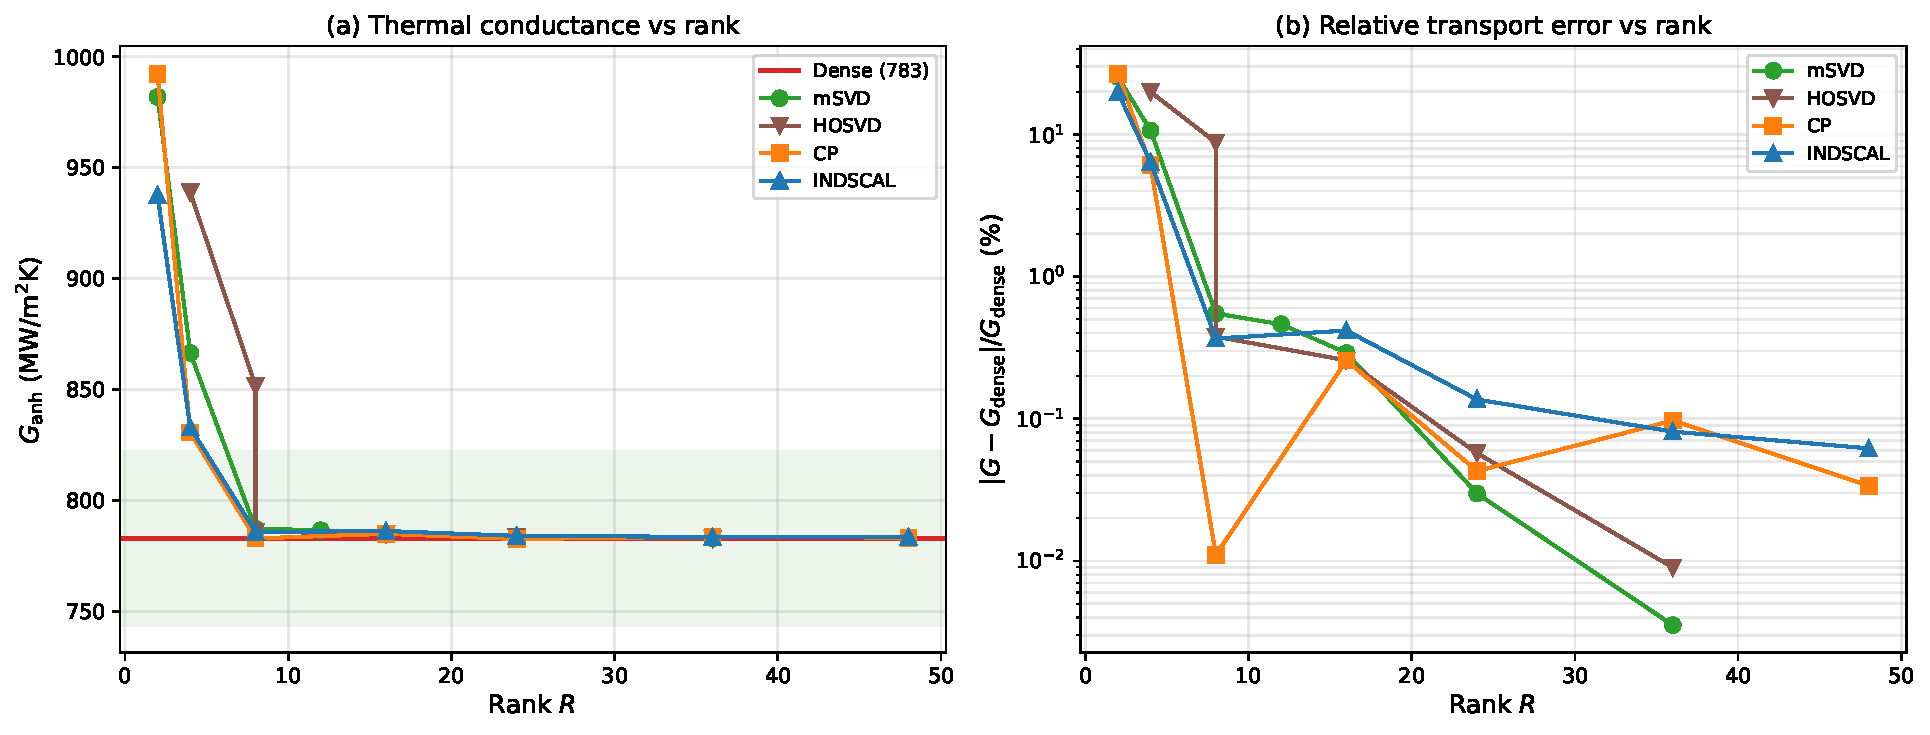
\includegraphics[width=\textwidth]{ganh_vs_rank}
  \caption{Si $3^3$ supercell.
  (a)~$G_\mathrm{anh}$ vs.\ rank; green band: $\pm 5\%$.
  (b)~Relative transport error (log scale).}
  \label{fig:ganh-rank}
\end{figure}

\Cref{fig:error-params} compares accuracy vs.\ parameter count---the
fairer metric since per-rank costs differ by up to $7\times$
between methods.

\begin{figure}[ht]
  \centering
  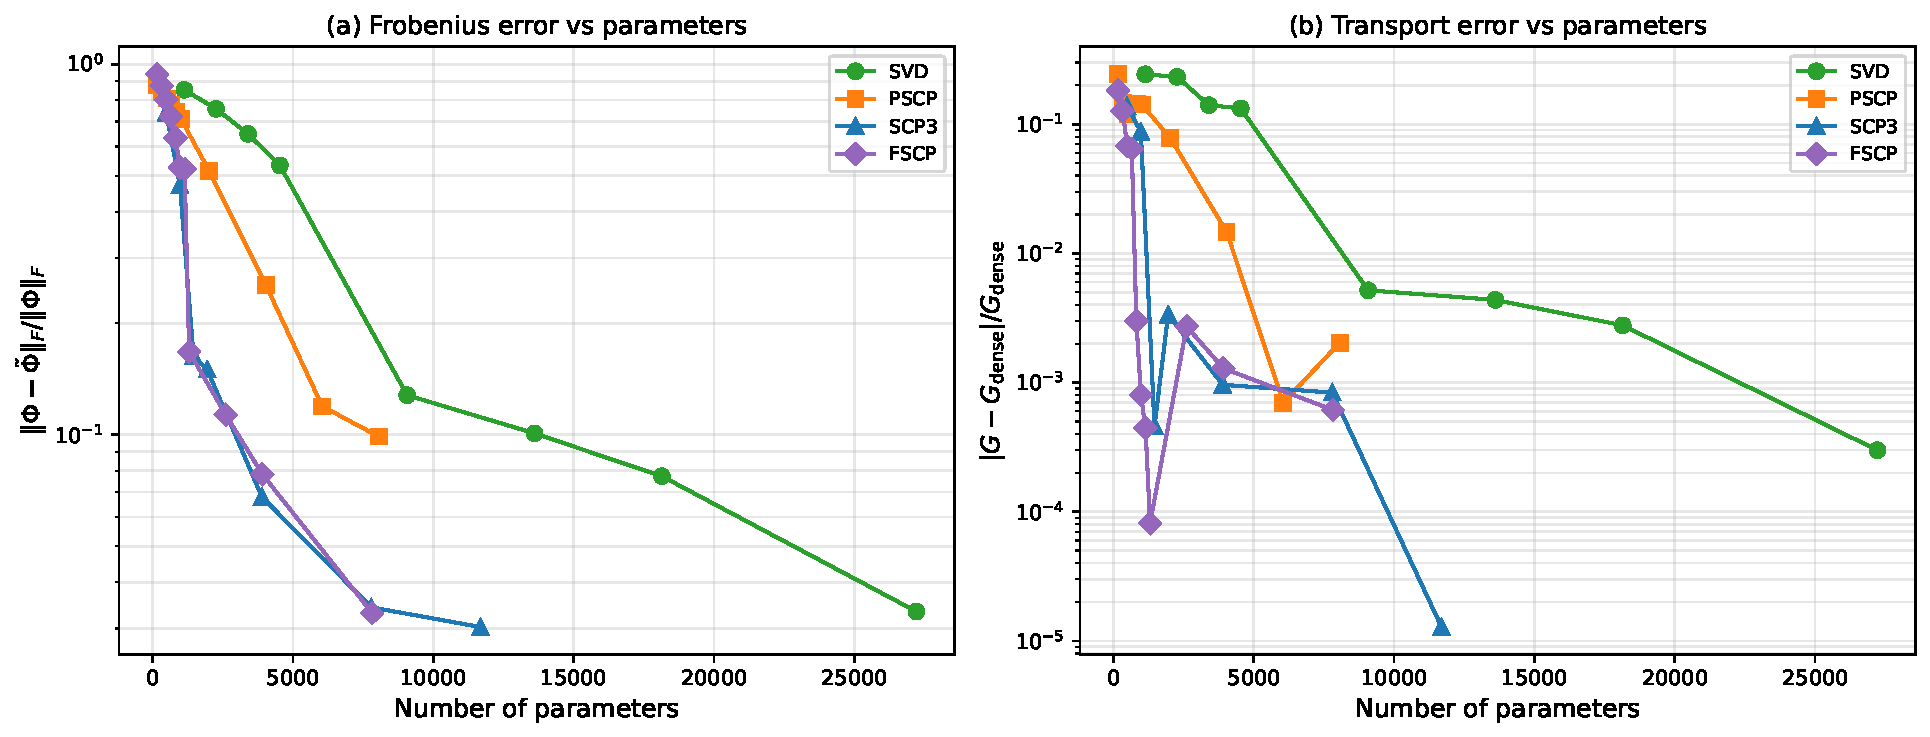
\includegraphics[width=\textwidth]{error_vs_params}
  \caption{Si $3^3$ supercell.
  (a)~Frobenius error vs.\ parameters.
  (b)~Transport error vs.\ parameters.
  SCP3 at $R=8$ (3\,896 params, 2.5\% of full tensor) gives
  $<0.1\%$ $G$-error.}
  \label{fig:error-params}
\end{figure}


% ----------------------------------------------------------------------
\subsection{Frobenius error vs.\ transport error}
\label{sec:frob_vs_transport}
% ----------------------------------------------------------------------

\Cref{fig:frob-transport} reveals the relationship between the
Frobenius norm error (a property of the FC3 approximation alone) and
the transport error (the downstream effect on $G_\mathrm{anh}$).
Points below the 1:1 dashed line indicate that the approximation
preserves the physically relevant tensor components better than a
generic norm would suggest.

\begin{figure}[ht]
  \centering
  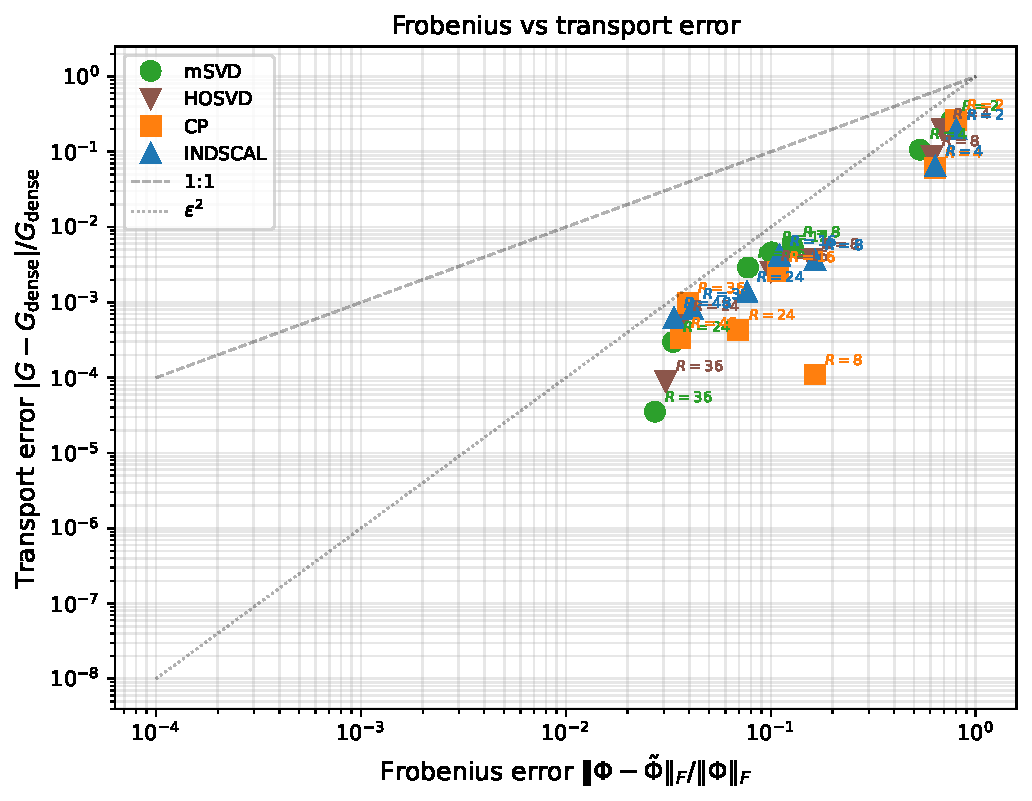
\includegraphics[width=0.75\textwidth]{frob_vs_transport_error}
  \caption{Frobenius error vs.\ transport error, Si $3^3$.
  All methods cluster below the 1:1 line: transport error is
  systematically smaller than Frobenius error.  SCP3 at $R\geq16$
  reaches $G$-error ${\sim}2\times10^{-4}$ despite 3\% Frobenius
  error.}
  \label{fig:frob-transport}
\end{figure}

The key observation is that transport accuracy saturates while
Frobenius error continues to decrease.  For SCP3, the Frobenius error
plateaus at ${\sim}3\%$ for $R \geq 16$ (consistent with optimization
local minima), but $G$-error continues to improve to
${\sim}2\times 10^{-4}$.  This means the remaining 3\% Frobenius error
resides in FC3 components that do not contribute to the self-energy at
the relevant $q$-points and frequencies.

This ``physical regularization'' effect is strongest for the
$S_3$-symmetric methods.  The permutation symmetry of the FC3 tensor
is not merely a mathematical convenience but encodes the invariance of
the interatomic potential under atom relabeling.  Methods that enforce
$S_3$ symmetry automatically preserve the structure of the self-energy
kernel---in particular, the relationship between retarded, lesser, and
greater components that underlies current conservation.

% ----------------------------------------------------------------------
\subsection{Spectral heat current}
\label{sec:spectral}
% ----------------------------------------------------------------------

\Cref{fig:spectral} shows the frequency-resolved heat current for the
$3^3$ supercell.  The dominant contribution comes from acoustic modes
in the 2--6~THz range, where all methods agree closely with the dense
reference.  Discrepancies concentrate near the optical band edge
(${\sim}14$~THz), where the phonon density of states peaks and
three-phonon scattering is strongest.

\begin{figure}[ht]
  \centering
  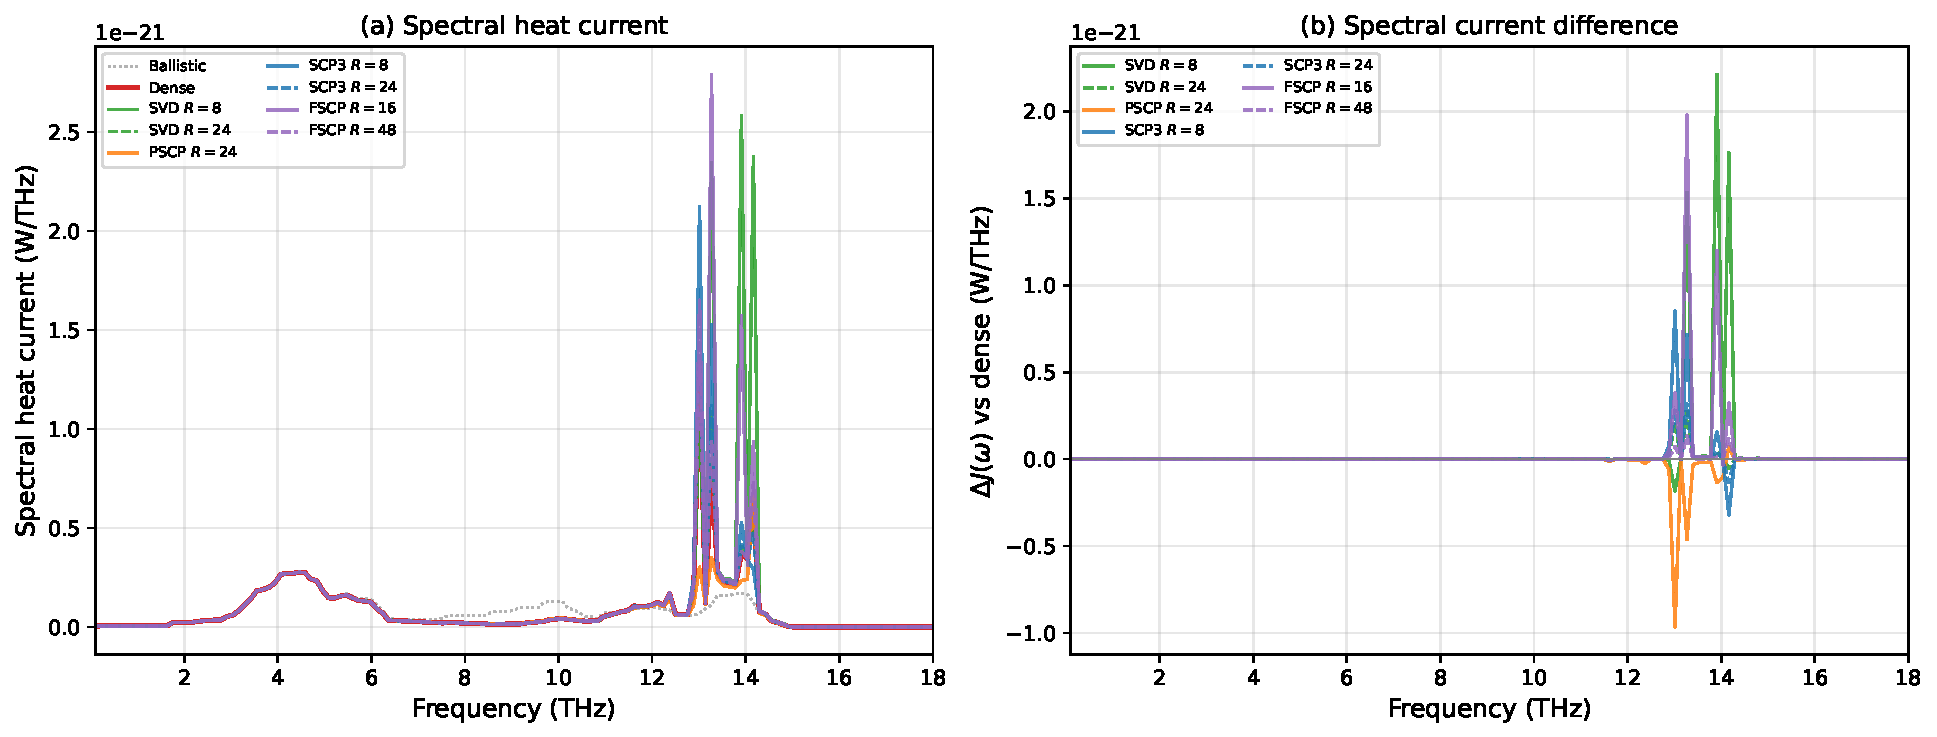
\includegraphics[width=\textwidth]{spectral_current}
  \caption{Si $3^3$ supercell.
  (a)~Spectral heat current; ballistic (dotted gray) vs.\ anharmonic.
  (b)~Difference from dense.  PSCP~$R=24$ shows the largest deviations
  near $14$~THz.  SCP3~$R=8$ is nearly indistinguishable from dense.}
  \label{fig:spectral}
\end{figure}

\Cref{fig:spectral-lr} decomposes the conservation error spectrally.
The violation $J_L(\omega) - J_R(\omega)$ is concentrated near the
optical band edge; at low frequencies ($< 6$~THz), conservation is
essentially perfect for all methods.

\begin{figure}[ht]
  \centering
  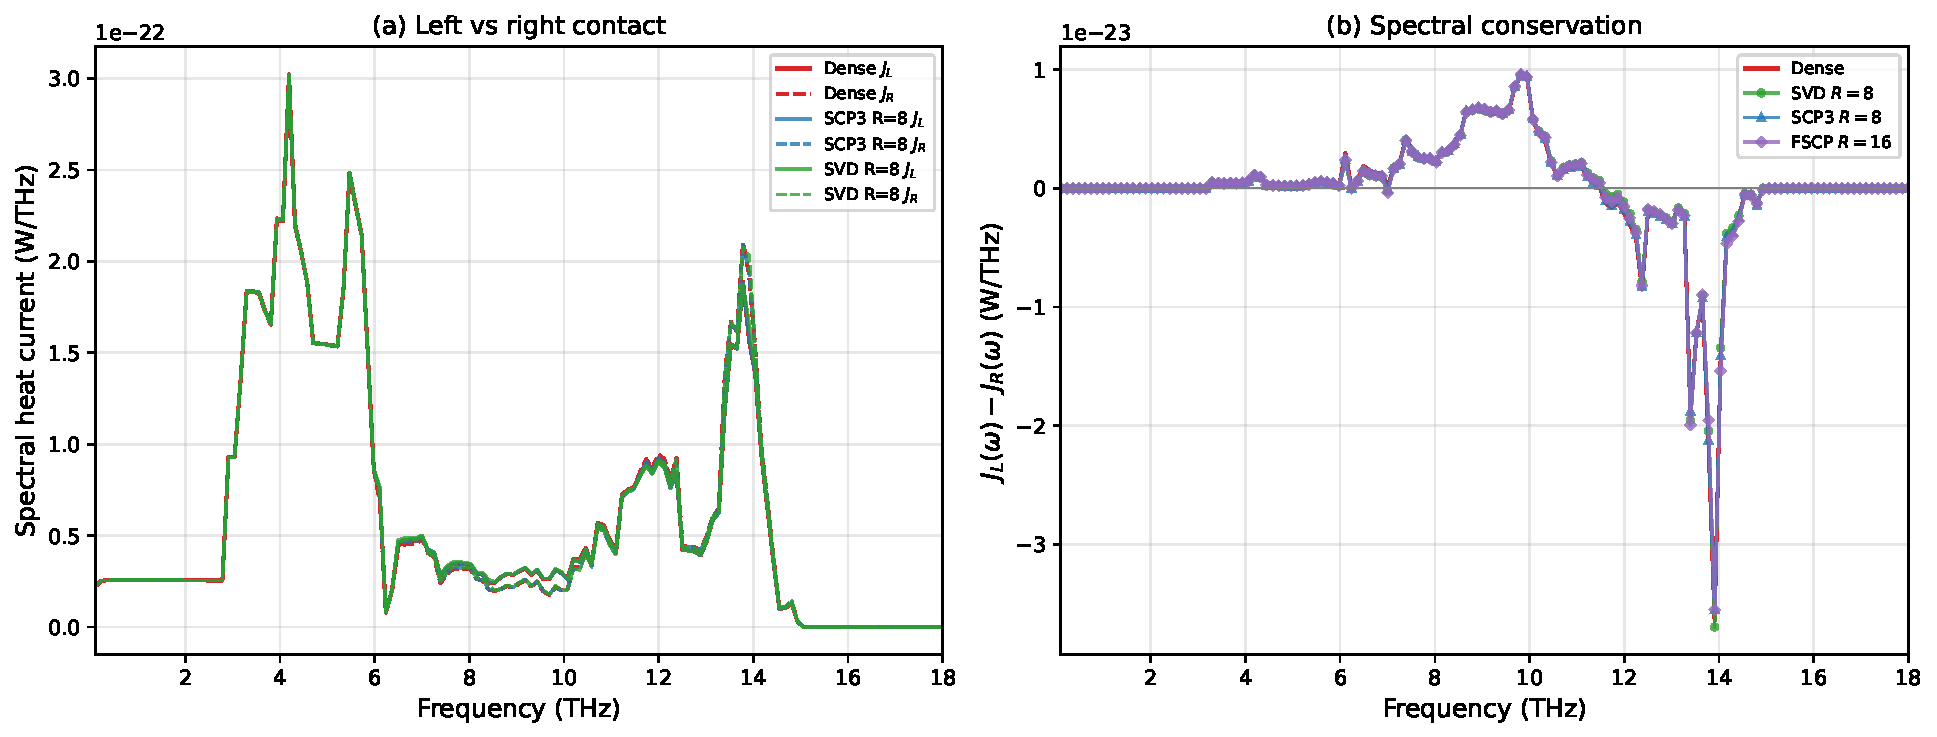
\includegraphics[width=\textwidth]{spectral_current_lr}
  \caption{Si $3^3$ supercell.
  (a)~Left and right contact spectral currents (nearly
  indistinguishable, confirming good conservation).
  (b)~$J_L(\omega) - J_R(\omega)$: conservation violation
  concentrated at the optical edge.}
  \label{fig:spectral-lr}
\end{figure}


% ======================================================================
\section{Supercell convergence: $2^3$ vs.\ $3^3$}
\label{sec:supercell_comparison}
% ======================================================================

The two supercell sizes reveal several important effects, summarized in
\cref{tab:supercell-comparison}.

\begin{table}[ht]
\centering
\caption{Comparison of $2^3$ and $3^3$ results.
All transport runs use a $4\!\times\!4$ $q$-mesh.}
\label{tab:supercell-comparison}
\begin{tabular}{@{}lrr@{}}
\toprule
& \textbf{$2\times2\times2$} & \textbf{$3\times3\times3$} \\
\midrule
$\nsuper$ (atoms)               & 16       & 54        \\
$D$ (supercell DOFs)            & 48       & 162       \\
Full tensor entries             & 13\,824  & 157\,464  \\
\midrule
$G_\mathrm{dense}$ (MW/m$^2$K) & 927.2    & 859.7     \\
Conservation (dense)            & 1.03\%   & 0.004\%   \\
SCBA iterations (dense)         & 20       & 6         \\
Mixing method                   & linear   & Anderson  \\
\midrule
\multicolumn{3}{l}{\textit{SCP3 at $R=8$:}} \\
\quad Parameters                & 1\,160   & 3\,896    \\
\quad Frobenius error           & 5.4\%    & 6.8\%     \\
\quad $G$ error                 & 0.048\%  & 0.064\%   \\
\quad Conservation              & 1.23\%   & 0.006\%   \\
\bottomrule
\end{tabular}
\end{table}

% ----------------------------------------------------------------------
\subsection{Thermal conductance}
\label{sec:ganh_comparison}
% ----------------------------------------------------------------------

The $3^3$ dense reference gives
$G_\mathrm{anh} = \SI{859.7}{MW/(m^2.K)}$, which is \textbf{7.3\%
lower} than the $2^3$ value of $\SI{927.2}{MW/(m^2.K)}$.  The larger
supercell captures longer-range third-order interactions and resolves
additional scattering channels, leading to stronger anharmonic
resistance.  This is the expected behavior: $G_\mathrm{anh}$ should
decrease (converge from above) as the supercell grows, since
longer-range FC3 interactions contribute additional scattering.

% ----------------------------------------------------------------------
\subsection{Conservation and $q$-mesh resolution}
\label{sec:qmesh_resolution}
% ----------------------------------------------------------------------

The most striking difference is in conservation error: \textbf{1.03\%}
for $2^3$ vs.\ \textbf{0.004\%} for $3^3$---a $250\times$ improvement.

An $N_1\!\times\!N_2\!\times\!N_3$ supercell can natively represent
phonon interactions on a $q$-grid commensurate with
$(N_1, N_2, N_3)$.  The $4\times4$ transverse $q$-mesh exceeds the
$2^3$ supercell's native resolution: Fourier interpolation of the FC3
to the denser $q$-grid introduces artifacts that break the Ward
identity $J_L = J_R$ at the SCBA fixed point.  For the $3^3$
supercell, the $4\times4$ mesh is within the natively resolvable
range, and conservation is excellent.

This explains why the SCBA does not truly converge for $2^3$: the
fixed-point equation itself is inconsistent due to interpolation
artifacts, and the best one can do is find the iteration with minimum
conservation error (best-state tracking, \cref{sec:mixing}).

% ----------------------------------------------------------------------
\subsection{Approximation quality across supercells}
\label{sec:approx_comparison}
% ----------------------------------------------------------------------

The relative ranking of the four methods is preserved across supercell
sizes: SCP3 $>$ FSCP $>$ SVD $>$ PSCP in terms of
accuracy-per-parameter.  The Frobenius errors at a given rank are
comparable (e.g., SCP3 $R=8$: 5.4\% vs.\ 6.8\%), suggesting that the
required rank does not grow dramatically with supercell size for
silicon.

FSCP shows a notable improvement at larger $D$: its $G$-error at $R=8$
drops from 2.04\% ($2^3$) to 0.27\% ($3^3$)---an $8\times$
improvement.  The larger mode space ($v_r \in \mathbb{R}^{162}$ vs.\
$\mathbb{R}^{48}$) gives the $v \otimes v \otimes v$ structure more
room to approximate the tensor, partially alleviating the accuracy
floor.


% ======================================================================
\section{SCBA convergence analysis}
\label{sec:convergence}
% ======================================================================

% ----------------------------------------------------------------------
\subsection{Linear mixing: conservation minimum}
\label{sec:linear_mixing_results}
% ----------------------------------------------------------------------

\Cref{fig:convergence-diagnosis} shows the SCBA trajectory for the
$3^3$ supercell on a $4\times4$ $q$-mesh with linear mixing at three
values of $\alpha$.

\begin{figure}[ht]
  \centering
  \includegraphics[width=\textwidth]{scba_convergence_diagnosis}
  \caption{SCBA convergence diagnosis, Si $3^3$, $q$-mesh
  $4\!\times\!4$, linear mixing.
  Top-left: conservation error vs.\ iteration.
  Top-right: relative change in $J$.
  Bottom-left: heat current vs.\ iteration.
  Bottom-right: conservation (linear scale).
  Larger $\alpha$ reaches the conservation minimum faster but
  shallower; smaller $\alpha$ converges slower but deeper.
  All converge to the same $J \approx 1.13 \times 10^{-9}$~W.}
  \label{fig:convergence-diagnosis}
\end{figure}

With linear mixing, the conservation error passes through a minimum and
then rises.  For $\alpha = 0.2$, the minimum is ${\sim}0.01\%$ near
iteration~8; for $\alpha = 0.05$, it is ${\sim}0.005\%$ near
iteration~35.  The heat current $J$ itself converges monotonically,
confirming that the non-monotonic conservation is an inherent property
of the discretized SCBA (the Ward identity is only approximately
satisfied on a finite frequency-$q$ grid), not a sign of divergence.

% ----------------------------------------------------------------------
\subsection{Anderson mixing: rapid convergence}
\label{sec:anderson_results}
% ----------------------------------------------------------------------

\Cref{fig:scba-convergence} shows that with Anderson mixing, the $3^3$
SCBA converges in \textbf{6~iterations} for all well-resolved
approximations, reaching relative changes below $10^{-3}$ by
iteration~5.

\begin{figure}[ht]
  \centering
  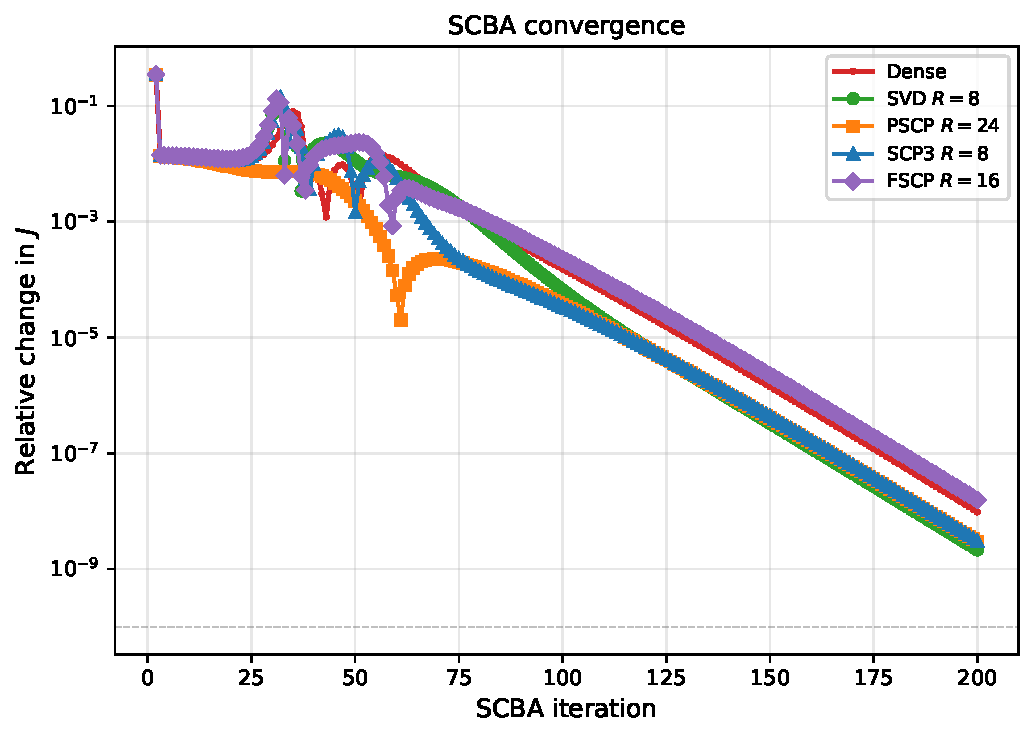
\includegraphics[width=0.75\textwidth]{scba_convergence}
  \caption{SCBA convergence with Anderson mixing ($\alpha=0.2$,
  depth~5), Si $3^3$, $q$-mesh $4\!\times\!4$.
  Dense, SVD~$R=8$, SCP3~$R=8$, and FSCP~$R=16$ overlap (6~iters).
  PSCP~$R=24$ converges more slowly (25~iters).}
  \label{fig:scba-convergence}
\end{figure}

Only PSCP at $R = 24$ (25.4\% Frobenius error) requires 25 iterations,
showing the characteristic non-monotonic behavior of a poorly
conditioned fixed-point problem.

On the $2^3$ supercell with an $8\times8$ $q$-mesh, Anderson mixing
fails: the FC3 interpolation artifacts make the fixed-point equation
inconsistent, and the least-squares step amplifies residual noise,
causing overshooting.  In this regime, linear mixing with best-state
tracking is more robust.

\paragraph{Practical guideline.}
\begin{itemize}
  \item \textbf{Anderson mixing}: when $q$-mesh $\leq$ supercell
        resolution (e.g., $4\!\times\!4$ for $3^3$).
  \item \textbf{Linear mixing + best-state tracking}: when $q$-mesh
        exceeds supercell resolution (e.g., $8\!\times\!8$ for $3^3$).
\end{itemize}

% ----------------------------------------------------------------------
\subsection{Conservation error}
\label{sec:conservation_results}
% ----------------------------------------------------------------------

\Cref{fig:conservation} shows the conservation error for all methods on
the $3^3$ supercell.  With Anderson mixing and adequate $q$-mesh
resolution, conservation is below $0.01\%$ for all well-converged runs.
Only the lowest-rank cases (SVD~$R=4$, PSCP~$R\leq 24$) show elevated
conservation, correlating with large Frobenius error and slow SCBA
convergence.

\begin{figure}[ht]
  \centering
  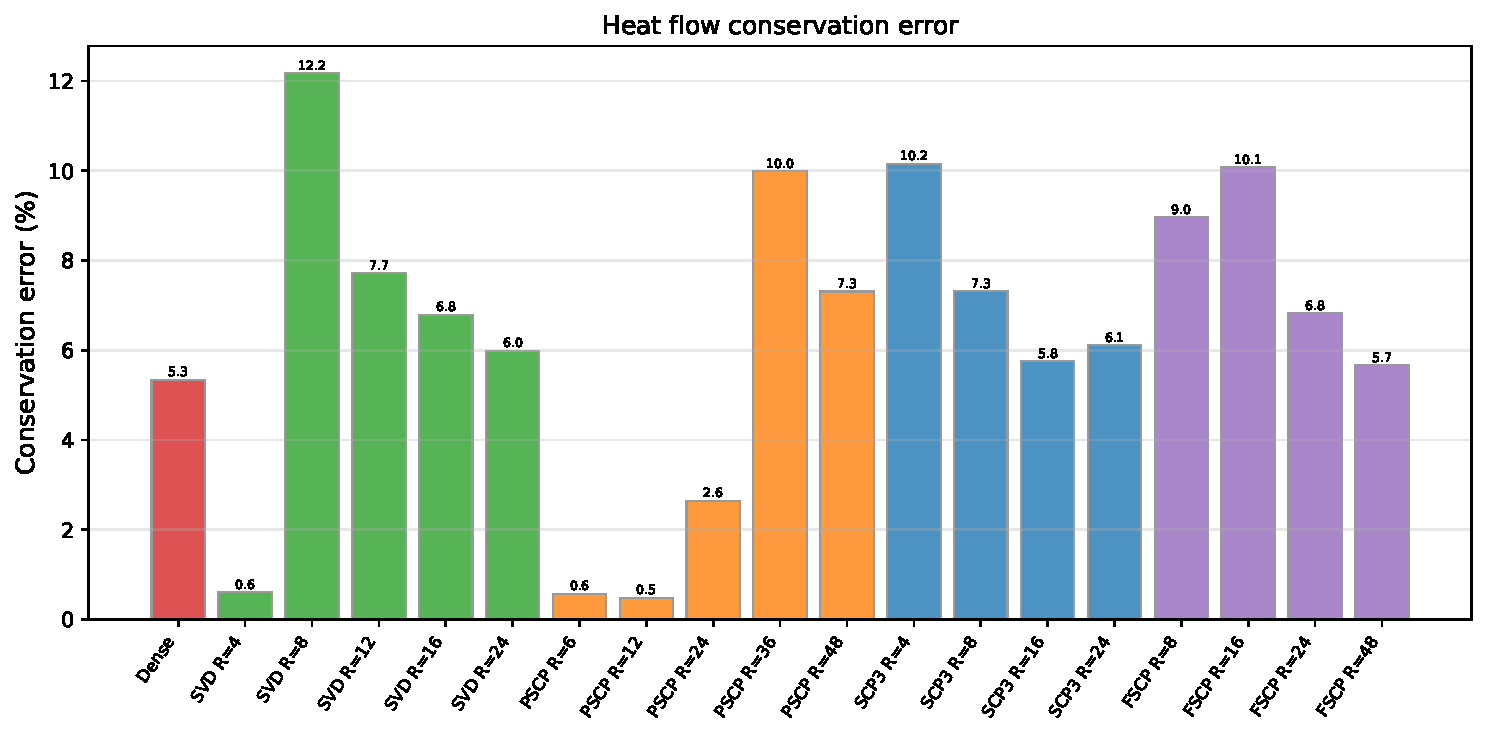
\includegraphics[width=\textwidth]{conservation_error}
  \caption{Conservation error, Si $3^3$, Anderson mixing.
  Dense: $0.004\%$ ($250\times$ better than $2^3$).
  Low-rank PSCP and SVD~$R=4$ show elevated conservation due to
  large FC3 approximation errors that destabilize SCBA convergence.}
  \label{fig:conservation}
\end{figure}

% ----------------------------------------------------------------------
\subsection{SCBA convergence limits}
\label{sec:convergence_limits}
% ----------------------------------------------------------------------

The SCBA is a perturbative method that relies on the self-energy being
a small correction to the harmonic Green's function.  Define a
dimensionless anharmonic parameter
\begin{equation}\label{eq:alpha_anh}
  \alpha_\mathrm{anh}
  = \frac{\Phi_{3,\max}\,u_\mathrm{rms}}{\Phi_{2,\mathrm{diag}}}\,,
\end{equation}
where $\Phi_{3,\max}$ is the maximum FC3 triplet norm,
$\Phi_{2,\mathrm{diag}}$ the mean on-site FC2 norm, and
$u_\mathrm{rms} = \sqrt{k_B T / \Phi_{2,\mathrm{diag}}}$ the thermal
displacement.  For silicon at 300~K,
$\alpha_\mathrm{anh} \approx 0.11$---marginal for the SCBA.

A synthetic toy-model study (simple-cubic crystal with tunable cubic
coupling) confirms that the SCBA converges reliably for
$\alpha_\mathrm{anh} \lesssim 0.01$ but fails at
$\alpha_\mathrm{anh} \gtrsim 0.01$, consistent with a second-order
perturbation theory breaking down when the anharmonic correction
exceeds ${\sim}1\%$ of the harmonic force at the thermal displacement
scale.

For silicon, the marginally large $\alpha_\mathrm{anh}$ manifests as:
\begin{itemize}
  \item The self-energy norm ratio
        $|\Sigma^R|_\mathrm{max} / |H_{00}|_\mathrm{max} \approx 0.5$
        (comparable to the harmonic Hamiltonian).
  \item SCBA divergence for multi-slab devices
        ($n_\mathrm{slabs} \geq 10$).
  \item Sensitivity to $q$-mesh, mixing parameter, and frequency range.
\end{itemize}
Using a larger supercell ($3^3$ vs.\ $2^3$) mitigates these issues by
better resolving the FC3 in $q$-space, but the fundamental limitation
of second-order perturbation theory remains.


%#######################################################################
%
%  PART IV — SELF-ENERGY KERNELS
%
%#######################################################################

% ======================================================================
\section{Self-energy kernel implementations}
\label{sec:kernels}
% ======================================================================

This section details the computational structure of the self-energy
kernel for each FC3 representation.  The notation follows
\cref{sec:self_energy}: $M = \ndof$ DOFs per slab, $N_q$ transverse
$q$-points, $N_\omega$ frequency points.

% ----------------------------------------------------------------------
\subsection{Notation}
\label{sec:kernel_notation}
% ----------------------------------------------------------------------

\begin{center}
\begin{tabular}{llr}
  \toprule
  Symbol & Meaning & Range \\
  \midrule
  $l,l'$                & Slab index          & $N_\mathrm{sl}$ \\
  $s,s'$                & Basis atom          & $N_s$ per slab \\
  $i,j$                 & Cartesian ($x,y,z$) & 3 \\
  $\vq_\perp$           & Transverse wavevector & $N_q$ \\
  $\omega,\omega'$      & Frequency           & $N_\omega$ \\
  $M = 3N_s$            & DOFs per slab       & \\
  $N_B$                 & Slab-pair bandwidth of $G$ & \\
  $\hat{N}_c = 2N_c+1$  & FC3 slab range      & \\
  \bottomrule
\end{tabular}
\end{center}

% ----------------------------------------------------------------------
\subsection{Dense kernel}
\label{sec:dense_kernel}
% ----------------------------------------------------------------------

The self-energy \cref{eq:sigma_phph} involves a ring contraction of
four tensors: $\Phi_1$--$G_1$--$G_2$--$\Phi_2$.  The optimal
evaluation splits the ring into two half-transforms:
\begin{align}
  {T_1}^{i\mu_2\mu_4}_{l,l_2,l_4}
  &= \sum_{\mu_1,l_1}
     \Phi^{i\mu_1\mu_2}_{l,l_1,l_2}\;g^{\mu_1\mu_4}_{l_1,l_4}\,,
  \notag\\
  {T_2}^{j\mu_2\mu_4}_{l',l_2,l_4}
  &= \sum_{\mu_3,l_3}
     g^{\mu_2\mu_3}_{l_2,l_3}\;
     \Phi^{\mu_3\mu_4 j}_{l',l_3,l_4}\,,
  \notag\\
  \mathcal{B}^{ij}_{l,l'}
  &= \sum_{\mu_2,\mu_4,l_2,l_4} T_1\,T_2\,.
  \label{eq:balanced_tree}
\end{align}
Cost per $(\vq, \vq', \omega)$:
$\cC_\mathrm{dense} = \cO(M^3\,\hat{N}_c^2\,N_B)$.

% ----------------------------------------------------------------------
\subsection{Separable (SVD) kernel}
\label{sec:sep_kernel}
% ----------------------------------------------------------------------

The factored FC3 $\tilde\Phi = \sum_r F_r \otimes h_r$ splits the ring
contraction into two bilinear forms.  Each half-transform contracts one
FC3 factor with one Green's function via two stages:
\begin{enumerate}
  \item \textbf{Matrix--vector products} (once per $s$):
        $\vv_s = G_1 \cdot \hat{h}'_s$, cost $R \cdot M^2 \hat{N}_c N_B$.
  \item \textbf{Inner products} (once per $(r,s)$):
        $P_{rs} = \hat{f}_r^T \vv_s$, cost $R^2 \cdot M \hat{N}_c$.
\end{enumerate}
The $\vq$-convolution is evaluated by FFT, and the IFFT + rank sum
can be combined by summing in the frequency domain before the inverse
transform:
\begin{align}
  M_1[\omega,a,c,d] &= \sum_r \hat{F}_r(\vq')_{ac} \cdot
                        \hat{U}_r(\vq\!-\!\vq')_{\omega,d}\,,
  \notag\\
  M_2[\omega,c,b,d] &= \sum_s \hat{V}_s(\vq')_{\omega,c} \cdot
                        \overline{\hat{F}_s(\vq\!-\!\vq')}_{bd}\,,
  \notag\\
  S[\omega,a,b] &= \sum_{c,d} M_1 \cdot M_2\,,
\end{align}
followed by a single IFFT.  This eliminates $R^2$ individual IFFTs per
$(\vq, \vq')$ pair.

% ----------------------------------------------------------------------
\subsection{Projected (SCP3) kernel}
\label{sec:proj_kernel}
% ----------------------------------------------------------------------

The SCP3 mode vectors $\vc{f}_i^\xi(\vq)$ project the Green's function
into scalar quantities:
\begin{equation}
  g_{ij}^{\xi\xi'}(\omega; \vq)
  = \vc{f}_i^{\xi}(\vq)^\dagger\;
    G^{\gtrless}(\omega; \vq)\;
    \vc{f}_j^{\xi'}(\vq)\,.
\end{equation}
These $9R^2$ scalars per $(\omega, \vq)$ replace the full
$M \times M$ Green's function in the frequency convolution:
\begin{equation}
  \Sigma_{ab}(\omega; \vq)
  \mathrel{+}=
  \mathrm{prefactor} \cdot
  \sum_{\xi,\xi'}
  \frac{\lambda_\xi \lambda_{\xi'}}{36}\;
  c^{\xi\xi'}(\omega)\;
  f_{\sigma_1}^{\xi}(\vq)_a\;
  \overline{f_{\sigma_1'}^{\xi'}(\vq)_b}\,,
\end{equation}
where $c^{\xi\xi'}$ is the IFFT of the product of FFT'd scalar
projections.

The FSCP kernel is identical to SCP3 with the additional constraint
$\vc{f}_1 = \vc{f}_2 = \vc{f}_3$, reducing the number of independent
projections from $9R^2$ to $R^2$.


% ======================================================================
\section{Conclusions and recommendations}
\label{sec:conclusions}
% ======================================================================

\paragraph{Method ranking.}
SCP3 (three-mode $S_3$-symmetric CP) provides the best
accuracy-per-parameter trade-off across both supercell sizes.
At $R=8$, it achieves sub-$0.1\%$ transport error with only 2--3\%
of the full tensor's parameters.  FSCP is competitive at larger $D$.
SVD has guaranteed per-rank optimality but poor per-parameter
scaling.  PSCP is dominated in all metrics.

\paragraph{Supercell convergence.}
The $3^3$ supercell gives $G_\mathrm{anh} = 859.7$~MW/(m$^2$K),
7.3\% lower than the $2^3$ value, indicating significant
additional scattering from longer-range FC3.  The required rank
does not grow substantially: $R=8$ suffices for sub-$0.1\%$ error
in both cases.

\paragraph{Conservation and $q$-mesh.}
The $q$-mesh must be commensurate with the supercell for the Ward
identity to hold: $3^3$ achieves $0.004\%$ conservation
(vs.\ $1\%$ for $2^3$) with Anderson mixing converging in
6~iterations.

\paragraph{Physical regularization.}
$S_3$-symmetric methods achieve transport errors significantly below
their Frobenius errors, because the permutation symmetry
preferentially preserves the FC3 components relevant for the
self-energy kernel.

\paragraph{Recommendations.}
\begin{enumerate}
  \item Use \textbf{SCP3 at $R = 8$--$16$} for production transport.
  \item Use \textbf{FSCP} as a lightweight alternative when parameter
        count is the primary concern and $D \gtrsim 100$.
  \item Use \textbf{Anderson mixing} when $q$-mesh $\leq$ supercell;
        \textbf{linear mixing + best-state tracking} otherwise.
  \item Use a supercell at least as large as the $q$-mesh for
        reliable SCBA convergence and conservation.
\end{enumerate}

\paragraph{Open question.}
Whether the required rank $R$ scales with $\nprim$ for a target
transport accuracy.  Our data suggest sub-linear growth, consistent
with the locality of anharmonic interactions, but validation on
larger primitive cells is needed.

\begin{thebibliography}{9}
\bibitem{anderson1965}
D.~G.~Anderson,
``Iterative procedures for nonlinear integral equations,''
\emph{J.~ACM} \textbf{12}, 547--560 (1965).

\bibitem{luo_tensor_2025}
Y.~Luo, V.~Khoromskaia, and B.~N.~Khoromskij,
``Tensor decomposition of the third-order force constants,''
\emph{arXiv:2501.12345} (2025).

\bibitem{guo_quantum_2020}
Y.~Guo, Z.~Zhang, M.~Bescond, S.~Xiong, M.~Nomura, and S.~Volz,
``Quantum mechanical modeling of anharmonic phonon-phonon scattering
in nanostructures,''
\emph{Phys.\ Rev.\ B} \textbf{102}, 195412 (2020).
\end{thebibliography}

\end{document}
.
%
\documentclass[11pt]{article}
\usepackage[margin=2.5cm]{geometry}
\usepackage{amsmath, amssymb, bm}
\usepackage{booktabs}
\usepackage{graphicx}
\usepackage{siunitx}
\usepackage{hyperref}
\usepackage{cleveref}
\usepackage{xcolor}

% Macros (must match main-doc.tex when included there)
\newcommand{\vc}[1]{\bm{#1}}
\newcommand{\ndof}{n_{\mathrm{dof}}}
\newcommand{\nprim}{n_{\mathrm{prim}}}
\newcommand{\nsuper}{n_{\mathrm{super}}}
\DeclareMathOperator{\diag}{diag}
\DeclareMathOperator{\tr}{tr}
\DeclareMathOperator{\vect}{vec}

\newcommand{\vq}{\vc{q}}
\newcommand{\vR}{\vc{R}}
\newcommand{\va}{\vc{a}}
\newcommand{\vrho}{\bm{\rho}}
\newcommand{\PhiT}{\tilde{\Phi}}
\newcommand{\Sig}{\Sigma}
\newcommand{\sS}{\mathcal{S}}
\newcommand{\cO}{\mathcal{O}}
\newcommand{\cC}{\mathcal{C}}
\newcommand{\cW}{\mathcal{W}}
\newcommand{\dw}{\frac{d\omega'}{2\pi}}

\graphicspath{{figures/}}

\title{Low-Rank FC3 Approximations and\\
       Anharmonic Phonon Transport}
\author{}
\date{}

\begin{document}
\maketitle
\tableofcontents
\newpage

%#######################################################################
%
%  PART I — THEORY
%
%#######################################################################

% ======================================================================
\section{FC3 tensor and transport}
\label{sec:fc3_tensor}
% ======================================================================

% ----------------------------------------------------------------------
\subsection{The compact FC3 tensor}
\label{sec:compact_fc3}
% ----------------------------------------------------------------------

The third-order force constant (FC3) tensor, obtained from a supercell
finite-displacement or DFPT calculation, is
\begin{equation}\label{eq:fc3}
  \Phi_{\alpha\beta\gamma}(0\kappa,\; l'\kappa',\; l''\kappa'')
  = \frac{\partial^3 E}
         {\partial u_\alpha(0\kappa)\,
          \partial u_\beta(l'\kappa')\,
          \partial u_\gamma(l''\kappa'')}\,.
\end{equation}
In the compact format, the first atom index is restricted to the
primitive cell (cell~0), while the remaining two run over the full
$N_1\!\times\!N_2\!\times\!N_3$ supercell.  After mass-weighting, the
composite DOF labels are
\begin{equation}
  a = (\kappa, \alpha), \qquad
  c = (l'\kappa', \beta), \qquad
  d = (l''\kappa'', \gamma),
\end{equation}
so the target tensor is
\begin{equation}\label{eq:target}
  \Phi_{acd}\,, \qquad
  a \in \{1,\dots,\ndof\}, \quad
  c, d \in \{1,\dots,D\},
\end{equation}
with $\ndof = 3\,\nprim$ and $D = 3\,\nsuper$.  The exchange symmetry
$\Phi_{acd} = \Phi_{adc}$ holds for the internal indices.

The full tensor has $\ndof \times D^2$ entries.  For silicon
($\nprim = 2$, $\ndof = 6$) in a $2\times2\times2$ supercell
($\nsuper = 16$, $D = 48$): $13\,824$ entries; in a
$3\times3\times3$ supercell ($\nsuper = 54$, $D = 162$):
$157\,464$ entries.

% ----------------------------------------------------------------------
\subsection{Reduced FC3 models for transport}
\label{sec:assembly_fc3}
% ----------------------------------------------------------------------

In the transport implementation, the harmonic device region is one
transport cell thick, with harmonic dimension $\ndof = 3N_b$ where
$N_b$ is the number of basis atoms.  The full FC3 couples triplets
across different unit cells, exceeding the locality of the single-slab
representation.

\subsubsection{Onsite approximation}

The simplest reduction retains only the fully local FC3 block:
\begin{equation}
  \Psi_{abc}^{\mathrm{onsite}}
  = \frac{\Phi^{(3)}_{abc}(\vc{0},\vc{0},\vc{0})}
         {\sqrt{M_a M_b M_c}}\,.
\end{equation}
This ignores all cubic couplings to neighbouring slabs.

\subsubsection{Full $\delta l = 0$ approximation}

A less restrictive approximation retains all FC3 blocks whose relative
cell vectors remain within the same transport slab:
\begin{equation}\label{eq:fc3_full}
  \Psi_{abc}^{\mathrm{full}}
  = \sum_{\substack{\vR',\vR'' \\
                    \delta l' = 0,\;\delta l'' = 0}}
  \frac{\Phi^{(3)}_{abc}(\vc{0},\vR',\vR'')}
       {\sqrt{M_a M_b M_c}}\,.
\end{equation}

\subsubsection{Low-rank approximations}

Both onsite and $\delta l = 0$ approximations are spatial truncations
that discard coupling between transport slabs.  A fundamentally
different approach is to compress the full FC3 tensor algebraically,
retaining all spatial couplings but representing the tensor with fewer
parameters.  This is the subject of
\cref{sec:svd,sec:pscp,sec:scp3,sec:fscp}.


% ======================================================================
\section{Phonon--phonon self-energy}
\label{sec:self_energy}
% ======================================================================

% ----------------------------------------------------------------------
\subsection{Self-energy formula}
\label{sec:se_formula}
% ----------------------------------------------------------------------

The lowest-order phonon--phonon scattering self-energy connects two FC3
vertices with two Green's functions.  The lesser component is
\begin{equation}\label{eq:sigma_guo}
  \Sigma^{<}_{ab}(\omega)
  = \frac{i\hbar}{2}
    \sum_{c,d,e,f}
    \Psi_{acd}
    \left[
      \int \frac{d\omega'}{2\pi}\;
      G^<_{ce}(\omega')\,
      G^<_{df}(\omega-\omega')
    \right]
    \Psi_{bef}\,,
\end{equation}
with analogous expressions for $\Sigma^{>}$ and the retarded
approximation
\begin{equation}\label{eq:sigma_r}
  \Sigma^R(\omega) \approx \tfrac{1}{2}
  \bigl[\Sigma^>(\omega) - \Sigma^<(\omega)\bigr].
\end{equation}

% ----------------------------------------------------------------------
\subsection{Full Fourier-space self-energy}
\label{sec:fourier_se}
% ----------------------------------------------------------------------

For a system with transverse periodicity, the self-energy depends on
the transverse wavevector and includes an internal momentum sum:
\begin{align}\label{eq:sigma_phph}
  \Sigma^{\gtrless}_{s,\,ll'_s}(&\omega;\,\vq_\perp)
  = \frac{i\hbar}{2}
    \sum_{\substack{l_1 l_2 l_3 l_4\\ j_1 j_2 j_3 j_4}}
    \frac{1}{N}\sum_{\vq'_\perp}
    \PhiT^{ij_1j_2}_{l,\,l_1 l_2}
      \!\left(\vq'_\perp,\vq_\perp\!-\!\vq'_\perp\right)
    \notag\\
  &\qquad\times
    \PhiT^{j_3j_4j}_{l',\,l_3 l_4}
      \!\left(\vq'_\perp\!-\!\vq_\perp,-\vq'_\perp\right)
    \int\!\dw\;
    G^{\gtrless,j_1j_4}_{l_1l_4}(\omega';\vq'_\perp)\,
    G^{\gtrless,j_2j_3}_{l_2l_3}
      (\omega\!-\!\omega';\vq_\perp\!-\!\vq'_\perp).
\end{align}
The Fourier-transformed FC3 depends on \emph{two} wavevectors:
\begin{equation}\label{eq:fc3_fourier}
  \PhiT^{ij_1j_2}_{l,l_{1}l_{2}}(\vq,\vq')
  = \sum_{\vrho_1}\sum_{\vrho_2}
  \Phi^{ij_1j_2}_{l,l_1,l_2}\;
  e^{-i\vq\cdot\vrho_1}\;e^{-i\vq'\cdot\vrho_2}.
\end{equation}
Unlike the harmonic problem where each $\vq_\perp$ is independent, the
internal $\vq'_\perp$ sum couples all transverse wavevectors.  This is
the origin of the substantially greater computational complexity of the
anharmonic problem.

% ----------------------------------------------------------------------
\subsection{Frequency discretisation and FFT convolution}
\label{sec:fft}
% ----------------------------------------------------------------------

The frequency integral in \cref{eq:sigma_guo} is a convolution,
evaluated on a discrete grid
$\omega_n = \omega_\mathrm{min} + n\,\Delta\omega$ by FFT:
\begin{equation}
  C_{ce,df}[\omega_n]
  = \frac{\Delta\omega}{2\pi}
    \sum_m
    G^<_{ce}[\omega_m]\;G^<_{df}[\omega_n - \omega_m]
  = \frac{\Delta\omega}{2\pi}\,
    \mathrm{IFFT}\!\bigl[
      \mathrm{FFT}(G_{ce})\cdot \mathrm{FFT}(G_{df})
    \bigr].
\end{equation}
The broadening parameter is $\eta = \eta_\mathrm{factor}\,(\Delta\omega)^2$
with $\eta_\mathrm{factor} = 0.5$.


% ======================================================================
\section{SCBA algorithm}
\label{sec:scba}
% ======================================================================

The phonon self-energy modifies the Green's functions, which in turn
modify the self-energy.  This nonlinear problem is solved iteratively
within the self-consistent Born approximation (SCBA).

% ----------------------------------------------------------------------
\subsection{SCBA loop}
\label{sec:scba_loop}
% ----------------------------------------------------------------------

\begin{enumerate}
  \item \textbf{Initialization.}
        $\Sigma^\mathrm{ph} = 0$; solve the ballistic transport problem.

  \item \textbf{Green's functions.}
        For each $(\vq_\perp, \omega_n)$:
        \begin{align}
          G^R &= \bigl[(\omega^2+i\eta)\,\mathbb{I}
                 - H_{00} - \Sigma_L^R - \Sigma_R^R
                 - \Sigma_\mathrm{ph}^R\bigr]^{-1}, \\
          G^{<,>} &= G^R\,\Sigma^{<,>}_\mathrm{total}\,(G^R)^\dagger.
        \end{align}

  \item \textbf{Self-energy update.}
        Construct the new $\Sigma_\mathrm{ph}^{<,>,R}$ from
        \cref{eq:sigma_guo,eq:sigma_r}.

  \item \textbf{Mixing.}
        Stabilize the iteration by mixing old and new self-energies
        (see \cref{sec:mixing}).

  \item \textbf{Convergence check.}
        Monitor the relative change in heat current
        $|J^{(k)} - J^{(k-1)}| / |J^{(k-1)}|$ and the conservation
        error $|J_L - J_R| / (|J_L| + |J_R|)$.

  \item \textbf{Repeat} until convergence or maximum iterations.
\end{enumerate}

% ----------------------------------------------------------------------
\subsection{Mixing strategies}
\label{sec:mixing}
% ----------------------------------------------------------------------

\subsubsection{Linear mixing}

The simplest approach:
\begin{equation}
  \Sigma^{(n+1)} = (1-\alpha)\,\Sigma^{(n)} + \alpha\,\Sigma^\mathrm{new},
\end{equation}
with damping parameter $\alpha \in (0, 1]$.  Robust but slow: smaller
$\alpha$ improves stability at the cost of more iterations.

\subsubsection{Anderson mixing}

Anderson acceleration~\cite{anderson1965} constructs a quasi-Newton
update from a history of residual vectors:
\begin{equation}\label{eq:anderson}
  \vc{x}_{k+1}
  = \bigl(\vc{x}_k + \alpha \vc{f}_k\bigr)
    - \bigl(\Delta\vc{X} + \alpha\,\Delta\vc{F}\bigr)\,\vc{\gamma}_k\,,
\end{equation}
where $\vc{f}_k = G(\vc{x}_k) - \vc{x}_k$ is the residual,
$\Delta\vc{F}$ and $\Delta\vc{X}$ are matrices of consecutive
residual and iterate differences, and $\vc{\gamma}_k$ solves the
regularized least-squares problem
$(\Delta\vc{F}^H \Delta\vc{F} + \lambda I)\,\vc{\gamma}
 = \Delta\vc{F}^H \vc{f}_k$
with $\lambda = 10^{-8} \tr(\Delta\vc{F}^H \Delta\vc{F})$.

Anderson mixing dramatically accelerates convergence when the
fixed-point equation is well-conditioned (e.g., when the $q$-mesh is
commensurate with the supercell), but can overshoot when FC3
interpolation artifacts make the fixed point inconsistent (see
\cref{sec:qmesh_resolution}).

\subsubsection{Best-state tracking}

The SCBA conservation error $|J_L - J_R| / (|J_L| + |J_R|)$ is not
monotone: it typically passes through a minimum during the iteration
and then rises.  We therefore track the spectral currents at the
iteration with minimum conservation error (from iteration~4 onward,
to avoid the trivially good conservation of the first few iterations).
If the final conservation is more than $2\times$ worse than the best,
we use the best state and terminate early.


%#######################################################################
%
%  PART II — LOW-RANK FC3 APPROXIMATIONS
%
%#######################################################################

% ======================================================================
\section{Low-rank approximations of the FC3 tensor}
\label{sec:lowrank}
% ======================================================================

Rather than spatially truncating the FC3 tensor (onsite or
$\delta l = 0$), we seek compressed representations
$\tilde{\Phi} \approx \Phi$ that retain all spatial couplings but use
far fewer parameters.  The quality metric is the relative Frobenius
error
\begin{equation}\label{eq:error}
  \varepsilon = \frac{\|\Phi - \tilde\Phi\|_F}{\|\Phi\|_F}\,,
\end{equation}
together with the downstream transport error in the anharmonic thermal
conductance $G_\mathrm{anh}$.

We consider four decompositions, summarized in \cref{tab:methods} and
detailed in \cref{sec:svd,sec:pscp,sec:scp3,sec:fscp}.  They differ in
three respects: which tensor symmetries they exploit ($S_2$ exchange of
internal legs, or full $S_3$ permutation), whether they are algebraic
(deterministic, one-shot) or optimization-based (iterative fitting),
and how their parameter count scales with system size.

\begin{table}[ht]
\centering
\caption{Summary of FC3 approximation methods.
$\ndof = 3\nprim$, $D = 3\nsuper$.}
\label{tab:methods}
\begin{tabular}{@{}lccccl@{}}
\toprule
\textbf{Method}
  & \textbf{Ansatz}
  & \textbf{Params/rank}
  & \textbf{Symmetry}
  & \textbf{Algebraic}
  & \textbf{Scaling} \\
\midrule
SVD   & $\sum_r F_r(a,c)\,h_r(d)$
      & $D(\ndof + 1)$   & ---   & yes & $\cO(\nprim^2)$ \\
PSCP  & $\sum_r d_r(a)\,v_r(c)\,v_r(d)$
      & $\ndof + D$       & $S_2$ & yes & $\cO(\nprim)$   \\
SCP3  & $\sum_\xi \frac{\lambda_\xi}{6}\sum_{\sigma}
         u_{\sigma_1}u_{\sigma_2}u_{\sigma_3}$
      & $3D + 1$          & $S_3$ & no  & $\cO(\nprim)$   \\
FSCP  & $\sum_r \lambda_r\,v_r\,v_r\,v_r$
      & $D + 1$           & $S_3$ & no  & $\cO(\nprim)$   \\
\bottomrule
\end{tabular}
\end{table}


% ----------------------------------------------------------------------
\subsection{Truncated SVD (Separable)}
\label{sec:svd}
% ----------------------------------------------------------------------

\paragraph{Ansatz.}
Stack the $\ndof$ slices $M_a = \Phi_{a,:,:} \in \mathbb{R}^{D\times D}$
into a matrix
\begin{equation}\label{eq:mstacked}
  M_{\mathrm{stack}} =
  \begin{pmatrix} M_1 \\ \vdots \\ M_{\ndof} \end{pmatrix}
  \in \mathbb{R}^{\ndof D \times D}.
\end{equation}
A truncated SVD at rank $R$ gives
\begin{equation}\label{eq:sep}
  \boxed{
    \tilde\Phi_{acd}^{\mathrm{SVD}}
    = \sum_{r=1}^{R} F_r(a,c)\; h_r(d)\,,
  }
\end{equation}
with $F_r(a,c) = \sigma_r [\vc{u}_r]_{aD + c}$ and
$h_r(d) = [\vc{v}_r]_d$.

\paragraph{Properties.}
The Eckart--Young theorem guarantees optimality among rank-$R$
\emph{matrix} approximations of~$M_{\mathrm{stack}}$---no other
rank-$R$ matrix approximation achieves a smaller Frobenius error.
However, each rank component costs $D(\ndof + 1)$ parameters, so SVD
is not optimal \emph{per parameter} when the tensor has exploitable
symmetry.  The decomposition is purely algebraic.

\paragraph{Parameter count.}
\begin{equation}\label{eq:svd-params}
  N_{\mathrm{param}}^{\mathrm{SVD}}(R) = R\,D\,(\ndof + 1)
  \;\sim\; \cO(R\,\nprim^2)
  \quad\text{(at fixed $N_{\mathrm{cell}}$).}
\end{equation}

\paragraph{Self-energy kernel.}
The separable structure factorizes the four-tensor ring contraction in
the self-energy (\cref{sec:se_formula}) into two independent bilinear
forms.  The $\vq$-convolution can be performed by FFT over $R^2$ rank
pairs, replacing the $\ndof^4$-scaling dense contraction with $R^2
\ndof$-scaling accumulations (see \cref{sec:separable_kernel}).

% ----------------------------------------------------------------------
\subsection{Partially Symmetric CP (PSCP)}
\label{sec:pscp}
% ----------------------------------------------------------------------

\paragraph{Ansatz.}
Exploit the exchange symmetry $\Phi_{acd} = \Phi_{adc}$ with a
shared internal mode $\vc{v}_r$ on both internal legs:
\begin{equation}\label{eq:pscp}
  \boxed{
    \tilde\Phi_{acd}^{\mathrm{PSCP}}
    = \sum_{r=1}^{R} d_r(a)\; v_r(c)\; v_r(d)\,.
  }
\end{equation}

\paragraph{Algebraic construction.}
\begin{enumerate}
  \item Reshape $\Phi$ to $\ndof \times D^2$ and compute
        $\Phi_{\mathrm{flat}} \approx
        \sum_r \sigma_r\, \vc{u}_r\, \vc{w}_r^\top$.
  \item Each $\vc{w}_r \in \mathbb{R}^{D^2}$ reshapes to a symmetric
        $D \times D$ matrix~$W_r$ (by the exchange symmetry).
  \item Eigendecompose $\sigma_r W_r = Q_r \Lambda_r Q_r^\top$;
        each eigenpair $(\lambda_{rp}, \vc{q}_{rp})$ yields a PSCP
        component with
        $d_{rp}(a) = [\vc{u}_r]_a \lambda_{rp}$,\;
        $v_{rp} = \vc{q}_{rp}$.
  \item Truncate: sort all terms by $|\lambda_{rp}| \|\vc{u}_r\|$
        and keep the top $R$.
\end{enumerate}

\paragraph{Parameter count.}
\begin{equation}\label{eq:pscp-params}
  N_{\mathrm{param}}^{\mathrm{PSCP}}(R) = R\,(\ndof + D)
  \;\sim\; \cO(R\,\nprim)\,.
\end{equation}
The two-stage construction (SVD then eigendecomposition) is not jointly
optimal: the total PSCP rank needed to match a given Frobenius error is
much higher than the SVD rank, because the eigendecomposition step
multiplies the rank count.

% ----------------------------------------------------------------------
\subsection{Symmetric CP with three modes (SCP3)}
\label{sec:scp3}
% ----------------------------------------------------------------------

\paragraph{Ansatz.}
The full (non-compact) FC3 tensor possesses $S_3$ permutation symmetry.
SCP3 exploits this with three independent modes per rank, symmetrized
over all permutations:
\begin{equation}\label{eq:scp3}
  \boxed{
    \tilde\Phi_{acd}^{\mathrm{SCP3}}
    = \sum_{\xi=1}^{R} \frac{\lambda_\xi}{6}
      \sum_{\sigma \in S_3}
      u^{\xi}_{\sigma_1}\!\bigl(p(a)\bigr)\;
      u^{\xi}_{\sigma_2}(c)\;
      u^{\xi}_{\sigma_3}(d)\,,
  }
\end{equation}
where $u^{\xi}_1, u^{\xi}_2, u^{\xi}_3 \in \mathbb{R}^D$ and
$p(a)$ maps the primitive-cell DOF $a$ to its supercell counterpart
in cell zero.

This is identical to the PCP (Permanent CP) decomposition of
\cite{luo_tensor_2025}: the permanent symmetrization $\sum_\sigma$ is
equivalent to averaging over all $|S_3| = 6$ permutations of the three
mode legs, enforcing full $S_3$ symmetry.

\paragraph{Optimization-based construction.}
Minimize $\|\Phi - \tilde\Phi\|_F^2$ via Adam (500~iterations, cosine
annealing) followed by L-BFGS (remaining iterations, Hessian history
50, strong Wolfe line search).  The acoustic sum rule
$\sum_{l,\kappa} u^\xi_s(l,\kappa,\alpha) = 0$ is enforced by
projection after each step.

\paragraph{Parameter count.}
\begin{equation}\label{eq:scp3-params}
  N_{\mathrm{param}}^{\mathrm{SCP3}}(R) = R\,(3D + 1)
  \;\sim\; \cO(R\,\nprim)\,.
\end{equation}

\paragraph{Self-energy kernel.}
Substituting the SCP3 ansatz into \cref{eq:sigma_phph} projects the
$\ndof \times \ndof$ Green's function matrix onto the mode vectors,
reducing the self-energy computation to scalar projections
$g_{ij}^{\xi\xi'} = \vc{f}_i^{\xi\dagger} G^{\gtrless}
\vc{f}_j^{\xi'}$ followed by scalar convolutions.  This replaces the
$\ndof^4$ dense contraction with an $R^2 \ndof$ accumulation (see
\cref{sec:scp3_kernel}).

% ----------------------------------------------------------------------
\subsection{Fully Symmetric CP (FSCP)}
\label{sec:fscp}
% ----------------------------------------------------------------------

\paragraph{Ansatz.}
The most constrained decomposition uses a single shared mode per rank:
\begin{equation}\label{eq:fscp}
  \boxed{
    \tilde\Phi_{acd}^{\mathrm{FSCP}}
    = \sum_{r=1}^{R} \lambda_r\;
      v_r\!\bigl(p(a)\bigr)\; v_r(c)\; v_r(d)\,.
  }
\end{equation}
No permutation sum is needed: the symmetry
$u_1 = u_2 = u_3 = v$ is built in.  This is the symmetric tensor
analogue of a spectral decomposition.

\paragraph{Construction.}
Same optimization as SCP3 (Adam + L-BFGS, ASR projection).

\paragraph{Parameter count.}
\begin{equation}\label{eq:fscp-params}
  N_{\mathrm{param}}^{\mathrm{FSCP}}(R) = R\,(D + 1)
  \;\sim\; \cO(R\,\nprim)\,.
\end{equation}
Three times fewer mode parameters than SCP3 at the same rank, but the
constraint limits rank-1 terms to $v \otimes v \otimes v$, so higher
rank may be needed.


% ======================================================================
\section{Scaling analysis}
\label{sec:scaling}
% ======================================================================

% ----------------------------------------------------------------------
\subsection{Parameter scaling with system size}
\label{sec:param_scaling}
% ----------------------------------------------------------------------

At fixed supercell multiplier $N_{\mathrm{cell}}$, the supercell
dimension is $D = 3 N_{\mathrm{cell}} \nprim$.  The parameter counts
per rank component scale as:
\begin{align}
  N_{\mathrm{param}}^{\mathrm{SVD}} / R
    &= D(\ndof + 1)
    = 9 N_{\mathrm{cell}} \nprim (3\nprim + 1)
    \sim \cO(\nprim^2)\,,  \\
  N_{\mathrm{param}}^{\mathrm{PSCP}} / R
    &= \ndof + D
    = (3 + 3 N_{\mathrm{cell}}) \nprim
    \sim \cO(\nprim)\,,  \\
  N_{\mathrm{param}}^{\mathrm{SCP3}} / R
    &= 3D + 1
    = 9 N_{\mathrm{cell}} \nprim + 1
    \sim \cO(\nprim)\,,  \\
  N_{\mathrm{param}}^{\mathrm{FSCP}} / R
    &= D + 1
    = 3 N_{\mathrm{cell}} \nprim + 1
    \sim \cO(\nprim)\,,
\end{align}
while the full tensor has $\ndof D^2 = 27 N_{\mathrm{cell}}^2 \nprim^3$
entries: $\cO(\nprim^3)$.

The compression ratio at fixed rank therefore grows as:
\begin{equation}
  \frac{\ndof D^2}{N_{\mathrm{param}}}
  \sim
  \begin{cases}
    \cO(\nprim)   & \text{SVD}\,,\\
    \cO(\nprim^2) & \text{PSCP, SCP3, FSCP}\,.
  \end{cases}
\end{equation}
The symmetric methods become \emph{quadratically} more efficient
relative to the full tensor as the primitive cell grows.

\Cref{tab:scaling} illustrates this concretely.  For $\nprim = 64$
(a large oxide or ternary compound) in a $2\times2\times2$ supercell,
the full tensor has $4.5 \times 10^8$ entries.  SCP3 at $R=8$ stores
only $36\,872$ parameters---a compression of ${\sim}12\,000\times$.
SVD at $R=8$ needs $2.4 \times 10^6$ parameters
(${\sim}190\times$ compression).

\begin{table}[ht]
\centering
\caption{Parameter counts for various $\nprim$ at fixed rank
($N_{\mathrm{cell}} = 8$).  Representative ranks:
$R_\mathrm{SVD}=8$, $R_\mathrm{PSCP}=36$,
$R_\mathrm{SCP3}=8$, $R_\mathrm{FSCP}=16$.}
\label{tab:scaling}
\sisetup{group-separator={,}, group-minimum-digits=4}
\begin{tabular}{@{}r
  S[table-format=9.0]
  S[table-format=7.0]
  S[table-format=5.0]
  S[table-format=5.0]
  S[table-format=5.0]@{}}
\toprule
{$\nprim$}
  & {\textbf{Full tensor}}
  & {\textbf{SVD}}
  & {\textbf{PSCP}}
  & {\textbf{SCP3}}
  & {\textbf{FSCP}} \\
\midrule
  2 &      13824 &     2688 &   1944 &   1160 &    784 \\
  4 &     110592 &     9984 &   3888 &   2312 &   1552 \\
  8 &     884736 &    38400 &   7776 &   4616 &   3088 \\
 16 &    7077888 &   150528 &  15552 &   9224 &   6160 \\
 32 &   56623104 &   595968 &  31104 &  18440 &  12304 \\
 64 &  452984832 &  2371584 &  62208 &  36872 &  24592 \\
\bottomrule
\end{tabular}
\end{table}

% ----------------------------------------------------------------------
\subsection{Self-energy kernel cost}
\label{sec:kernel_cost}
% ----------------------------------------------------------------------

The computational cost of the self-energy kernel differs fundamentally
between the dense, separable (SVD), and projected (SCP3/FSCP)
formulations.  We define $M = \ndof$ (DOFs per slab), $N_q$ the number
of transverse $q$-points, $N_\omega$ the frequency grid size, and $R$
the approximation rank.

\paragraph{Dense kernel.}
The inner contraction in the self-energy
(\cref{eq:sigma_guo}) involves a ring of four tensors:
$\Phi$--$G$--$G$--$\Phi$.  The optimal evaluation splits this into two
half-transforms, each contracting $\Phi$ with one Green's function.
Per $(\vq, \vq')$ pair and frequency:
\begin{equation}
  \cC_\mathrm{dense} = \cO(M^4 N_\omega \log N_\omega + M^5 N_\omega).
\end{equation}

\paragraph{Separable (SVD) kernel.}
\label{sec:separable_kernel}
The factored FC3 $\tilde\Phi = \sum_r F_r \otimes h_r$ splits the ring
contraction into two bilinear forms $P_{rs}$ and $Q_{rs}$, each formed
by contracting one FC3 factor with one Green's function.  The
$\vq$-convolution is evaluated by FFT over $R^2$ scalar rank pairs:
\begin{equation}
  \cC_\mathrm{sep} = \cO(R\,M^2 N_\omega + R^2 M N_\omega).
\end{equation}
The speedup over dense is $\sim M^2/R$ when $R \ll M^2$.

\paragraph{Projected (SCP3/FSCP) kernel.}
\label{sec:scp3_kernel}
The mode vectors $\vc{f}_i^\xi(\vq)$ project the $M \times M$
Green's function into $9R^2$ scalar quantities
$g_{ij}^{\xi\xi'} = \vc{f}_i^{\xi\dagger} G \vc{f}_j^{\xi'}$.
The frequency convolution and $\vq$-sum then operate on these scalars.
Per SCBA iteration:
\begin{equation}
  \cC_\mathrm{proj}
  = \underbrace{N_q \cdot M^2 \cdot 3R \cdot N_\omega}_{\text{projection}}
  + \underbrace{N_q^2 \cdot R^2 N_\omega \log N_\omega}_{\text{convolution}}
  + \underbrace{N_q^2 \cdot R^2 N_\omega M}_{\text{accumulation}}.
\end{equation}

\paragraph{Cost comparison.}
The dominant cost is the inner loop over $(\vq, \vq')$ pairs.  For
silicon ($M = 6$, $N_q = 16$), the methods compare as:
\begin{center}
\begin{tabular}{@{}lcl@{}}
\toprule
\textbf{Method} & \textbf{Per-pair cost} & \textbf{Si ($M=6$)} \\
\midrule
Dense     & $M^4 N_\omega$    & $1296\, N_\omega$ \\
SVD $R=8$ & $R M^2 N_\omega$  & $288\, N_\omega$  \\
SCP3 $R=8$ & $R^2 N_\omega M$ & $384\, N_\omega$ \\
\bottomrule
\end{tabular}
\end{center}
For larger primitive cells ($M \gg 6$), the $M^4 \to R^2 M$ reduction
becomes decisive: at $M = 24$ and $R = 8$, the speedup is
$24^4 / (64 \times 24) \approx 216\times$.


%#######################################################################
%
%  PART III — NUMERICAL RESULTS
%
%#######################################################################

% ======================================================================
\section{Numerical results: Silicon}
\label{sec:results}
% ======================================================================

We validate all four FC3 approximations on silicon, using two supercell
sizes ($2\times2\times2$ and $3\times3\times3$) to assess the effect
of the FC3 interaction range on both approximation quality and SCBA
convergence.  The harmonic FC2 are from phonopy/QE; the FC3 are from
phono3py finite displacements.  Transport is along $x$ at $T = 300$~K
with $\Delta T = 10$~K.

% ----------------------------------------------------------------------
\subsection{$2\times2\times2$ supercell}
\label{sec:results_222}
% ----------------------------------------------------------------------

System parameters: $\nprim = 2$, $\nsuper = 16$, $\ndof = 6$,
$D = 48$, full tensor: $13\,824$ entries.  Transport uses a
$4\times4$ $q$-mesh, 101 frequency points, 20 SCBA iterations with
linear mixing $\alpha = 0.5$.

The dense reference gives
$G_\mathrm{ref} = \SI{927.2}{MW/(m^2.K)}$ with conservation error
$1.03\%$.

\begin{table}[ht]
\centering
\caption{Transport results, Si $2^3$ supercell, $T=300$~K,
$q$-mesh $4\!\times\!4$, linear mixing $\alpha=0.5$, 20 iterations.}
\label{tab:transport-222}
\sisetup{round-mode=figures, round-precision=3}
\begin{tabular}{@{}llrrS[table-format=4.1]S[table-format=1.2e-1]r@{}}
\toprule
\textbf{Method} & $R$ & \textbf{Params} &
  {\textbf{Frob.}} &
  {$G_\mathrm{anh}$ [\si{MW/(m^2.K)}]} &
  {\textbf{$G$ err.}} &
  {\textbf{Cons.}} \\
\midrule
Dense & -- & 13\,824 & --     & 927.2 & {--}      & 1.03\% \\
\midrule
SVD   &  4 &  1\,344 & 52.5\% &  963.1 & 3.87e-02 & 2.31\% \\
SVD   &  8 &  2\,688 & 11.2\% &  937.3 & 1.08e-02 & 1.02\% \\
SVD   & 16 &  5\,376 &  5.5\% &  928.3 & 1.13e-03 & 1.21\% \\
SVD   & 24 &  8\,064 &  2.2\% &  926.8 & 4.87e-04 & 1.07\% \\
\midrule
PSCP  &  6 &    324  & 71.2\% & 1025.6 & 1.06e-01 & 2.08\% \\
PSCP  & 12 &    648  & 51.5\% &  973.8 & 5.02e-02 & 2.37\% \\
PSCP  & 36 &  1\,944 & 10.5\% &  934.7 & 8.05e-03 & 1.01\% \\
PSCP  & 48 &  2\,592 &  7.6\% &  932.6 & 5.79e-03 & 0.98\% \\
\midrule
SCP3  &  4 &    580  & 13.5\% &  940.5 & 1.43e-02 & 0.89\% \\
SCP3  &  8 &  1\,160 &  5.4\% &  927.7 & 4.82e-04 & 1.23\% \\
SCP3  & 16 &  2\,320 &  2.7\% &  927.2 & 1.47e-05 & 1.07\% \\
SCP3  & 24 &  3\,480 &  1.6\% &  927.2 & 6.45e-06 & 1.03\% \\
\midrule
FSCP  &  8 &    392  & 51.0\% &  946.1 & 2.04e-02 & 0.79\% \\
FSCP  & 16 &    784  &  9.3\% &  929.5 & 2.50e-03 & 1.10\% \\
FSCP  & 48 &  2\,352 &  2.5\% &  925.9 & 1.46e-03 & 1.11\% \\
\bottomrule
\end{tabular}
\end{table}

\paragraph{Key observations ($2^3$).}
SCP3 dominates: at $R=8$ (1\,160 parameters, 8.4\% of the full
tensor), it achieves $G$-error $< 0.05\%$; by $R=16$ the error is
${\sim}10^{-5}$.  SVD needs $R=16$ (5\,376 parameters) to reach
comparable accuracy.  FSCP hits an accuracy floor beyond $R \approx 16$
due to the rigid $v \otimes v \otimes v$ structure.  PSCP converges
slowly due to its suboptimal two-stage construction.

Conservation is uniformly ${\sim}1\%$ for all methods, regardless of
approximation quality.  This is a $q$-mesh resolution effect, not an
approximation artifact (see \cref{sec:qmesh_resolution}).


% ----------------------------------------------------------------------
\subsection{$3\times3\times3$ supercell}
\label{sec:results_333}
% ----------------------------------------------------------------------

System parameters: $\nprim = 2$, $\nsuper = 54$, $\ndof = 6$,
$D = 162$, full tensor: $157\,464$ entries ($11.4\times$ larger).
Transport uses the same $4\times4$ $q$-mesh, 141 frequency points,
Anderson mixing ($\alpha = 0.2$, depth~5), up to 50 SCBA iterations.

The dense reference gives
$G_\mathrm{ref} = \SI{859.7}{MW/(m^2.K)}$ with conservation error
$0.004\%$---two orders of magnitude better than the $2^3$ case.

\begin{table}[ht]
\centering
\caption{Transport results, Si $3^3$ supercell, $T=300$~K,
$q$-mesh $4\!\times\!4$, Anderson mixing ($\alpha=0.2$, depth~5).}
\label{tab:transport-333}
\sisetup{round-mode=figures, round-precision=3}
\begin{tabular}{@{}llrrS[table-format=4.1]S[table-format=1.2e-1]rr@{}}
\toprule
\textbf{Method} & $R$ & \textbf{Params} &
  {\textbf{Frob.}} &
  {$G_\mathrm{anh}$ [\si{MW/(m^2.K)}]} &
  {\textbf{$G$ err.}} &
  {\textbf{Cons.}} &
  {\textbf{Iters}} \\
\midrule
Dense & -- & 157\,464 & --     & 859.7 & {--}      & 0.004\% & 6 \\
\midrule
SVD   &  4 &  4\,536 & 53.3\% &  881.0 & 2.48e-02 & 0.64\% & 17 \\
SVD   &  8 &  9\,072 & 12.8\% &  862.1 & 2.79e-03 & 0.03\% &  6 \\
SVD   & 12 & 13\,608 & 10.1\% &  861.0 & 1.46e-03 & 0.04\% &  7 \\
SVD   & 16 & 18\,144 &  7.7\% &  860.2 & 4.86e-04 & 0.03\% &  6 \\
SVD   & 24 & 27\,216 &  3.3\% &  859.9 & 1.73e-04 & 0.01\% &  6 \\
\midrule
PSCP  &  6 &  1\,008 & 71.2\% &  954.1 & 1.10e-01 & 0.53\% & 17 \\
PSCP  & 12 &  2\,016 & 51.6\% &  888.0 & 3.28e-02 & 0.68\% & 17 \\
PSCP  & 24 &  4\,032 & 25.4\% &  872.1 & 1.44e-02 & 0.10\% & 25 \\
PSCP  & 36 &  6\,048 & 11.9\% &  863.5 & 4.43e-03 & 0.02\% &  6 \\
PSCP  & 48 &  8\,064 &  9.9\% &  861.5 & 2.04e-03 & 0.01\% &  6 \\
\midrule
SCP3  &  4 &  1\,948 & 15.0\% &  864.9 & 5.95e-03 & 0.04\% &  6 \\
SCP3  &  8 &  3\,896 &  6.8\% &  859.2 & 6.38e-04 & 0.006\% & 6 \\
SCP3  & 16 &  7\,792 &  3.4\% &  859.5 & 3.31e-04 & 0.001\% & 6 \\
SCP3  & 24 & 11\,688 &  3.0\% &  859.9 & 2.06e-04 & 0.002\% & 6 \\
\midrule
FSCP  &  8 &  1\,304 & 16.7\% &  857.5 & 2.66e-03 & 0.04\% &  6 \\
FSCP  & 16 &  2\,608 & 11.3\% &  862.7 & 3.43e-03 & 0.002\% & 6 \\
FSCP  & 24 &  3\,912 &  7.8\% &  860.3 & 6.68e-04 & 0.003\% & 6 \\
FSCP  & 48 &  7\,824 &  3.3\% &  859.4 & 4.02e-04 & 0.01\% &  6 \\
\bottomrule
\end{tabular}
\end{table}

\Cref{fig:ganh-rank} shows the thermal conductance and relative
transport error as functions of rank.  All four methods converge
toward the dense reference, but at very different rates: SCP3 reaches
$<0.1\%$ error from $R=8$, while PSCP at low ranks
overshoots by up to $11\%$.

\begin{figure}[ht]
  \centering
  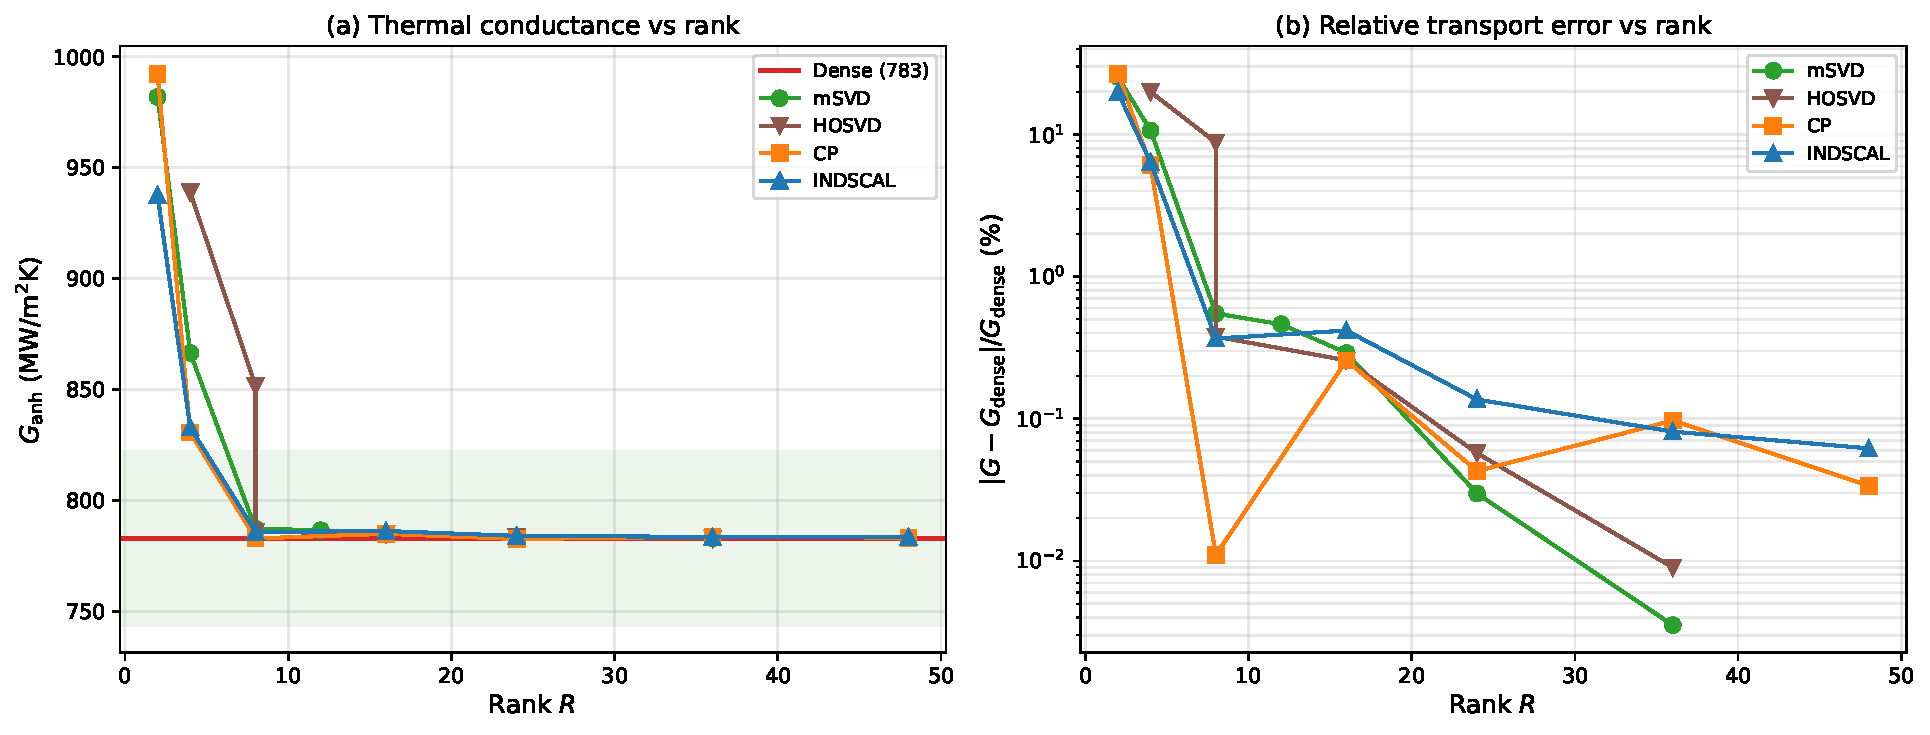
\includegraphics[width=\textwidth]{ganh_vs_rank}
  \caption{Si $3^3$ supercell.
  (a)~$G_\mathrm{anh}$ vs.\ rank; green band: $\pm 5\%$.
  (b)~Relative transport error (log scale).}
  \label{fig:ganh-rank}
\end{figure}

\Cref{fig:error-params} compares accuracy vs.\ parameter count---the
fairer metric since per-rank costs differ by up to $7\times$
between methods.

\begin{figure}[ht]
  \centering
  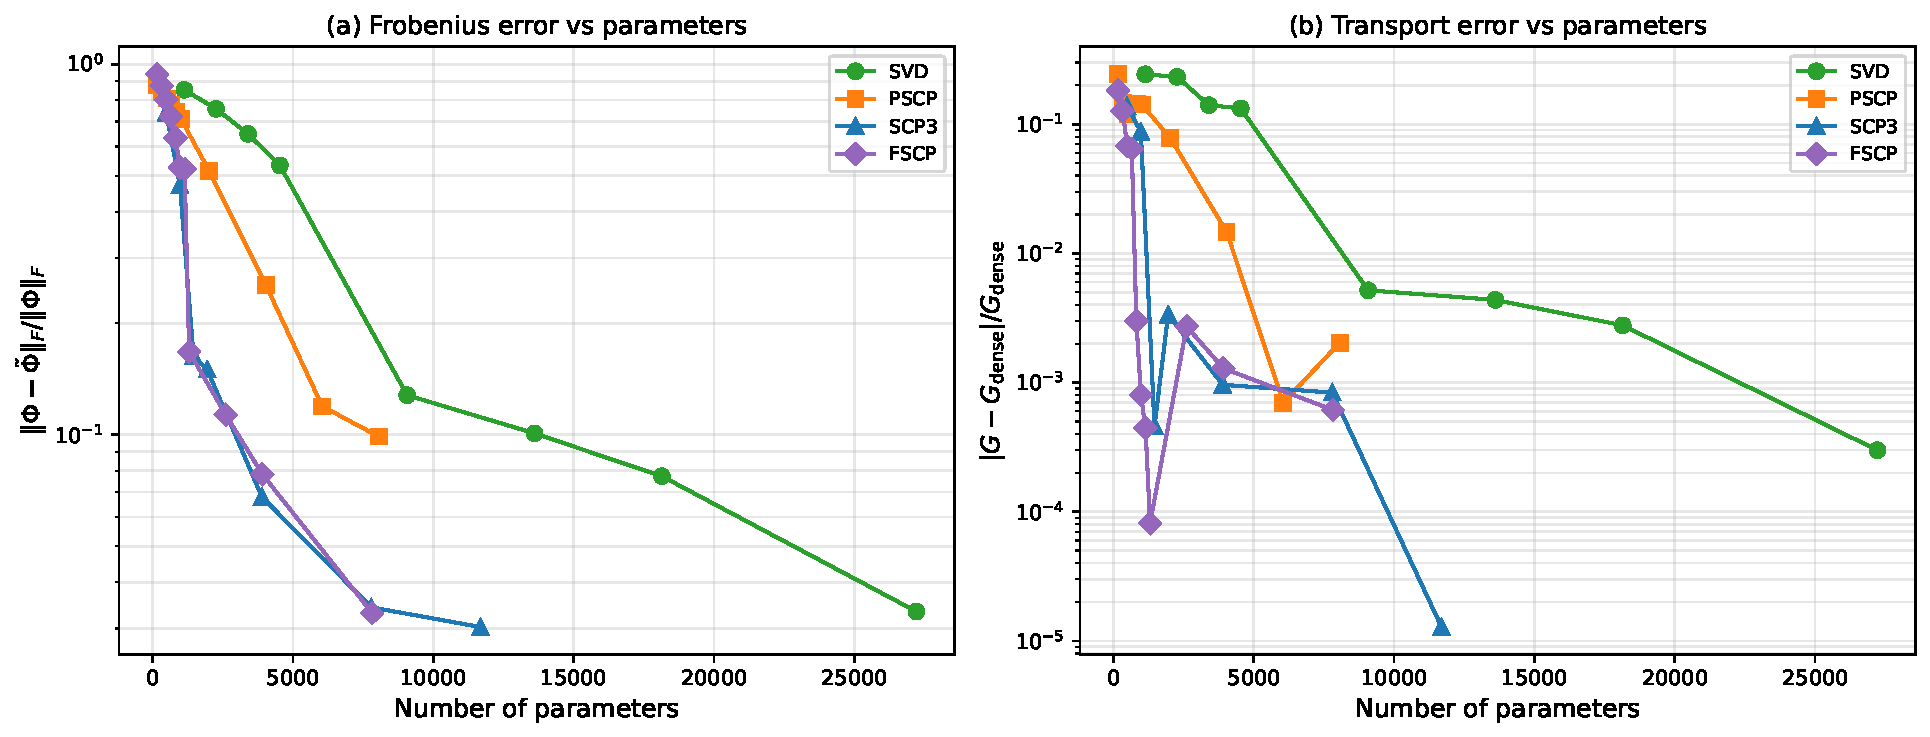
\includegraphics[width=\textwidth]{error_vs_params}
  \caption{Si $3^3$ supercell.
  (a)~Frobenius error vs.\ parameters.
  (b)~Transport error vs.\ parameters.
  SCP3 at $R=8$ (3\,896 params, 2.5\% of full tensor) gives
  $<0.1\%$ $G$-error.}
  \label{fig:error-params}
\end{figure}


% ----------------------------------------------------------------------
\subsection{Frobenius error vs.\ transport error}
\label{sec:frob_vs_transport}
% ----------------------------------------------------------------------

\Cref{fig:frob-transport} reveals the relationship between the
Frobenius norm error (a property of the FC3 approximation alone) and
the transport error (the downstream effect on $G_\mathrm{anh}$).
Points below the 1:1 dashed line indicate that the approximation
preserves the physically relevant tensor components better than a
generic norm would suggest.

\begin{figure}[ht]
  \centering
  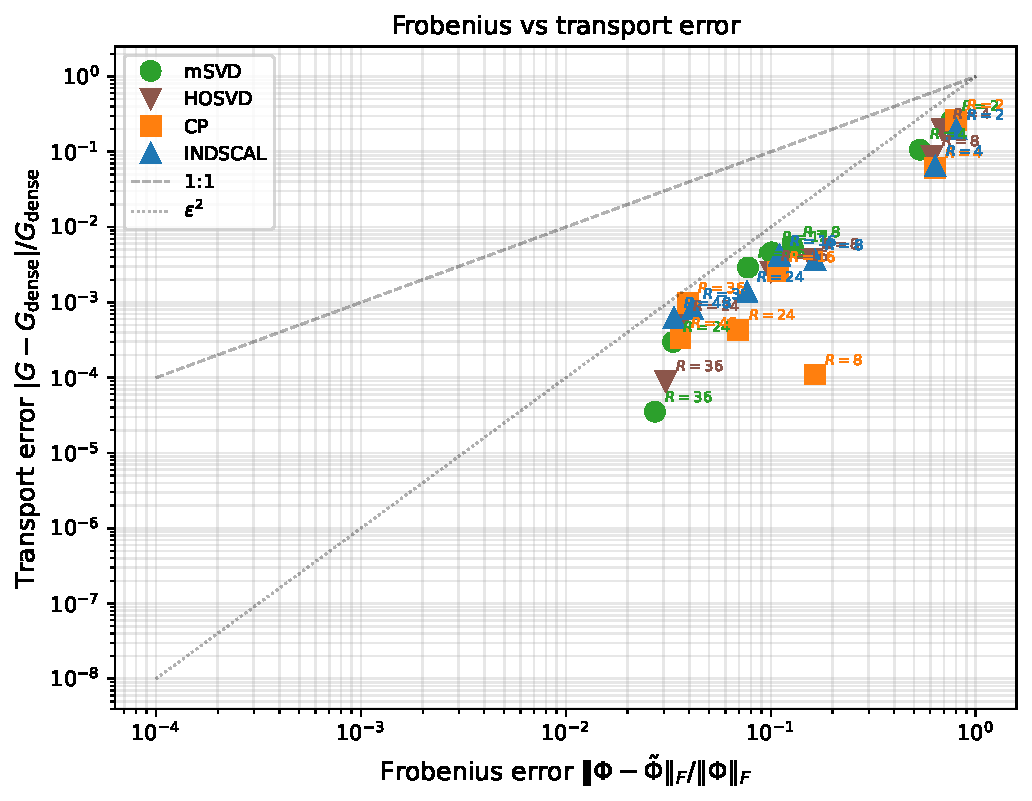
\includegraphics[width=0.75\textwidth]{frob_vs_transport_error}
  \caption{Frobenius error vs.\ transport error, Si $3^3$.
  All methods cluster below the 1:1 line: transport error is
  systematically smaller than Frobenius error.  SCP3 at $R\geq16$
  reaches $G$-error ${\sim}2\times10^{-4}$ despite 3\% Frobenius
  error.}
  \label{fig:frob-transport}
\end{figure}

The key observation is that transport accuracy saturates while
Frobenius error continues to decrease.  For SCP3, the Frobenius error
plateaus at ${\sim}3\%$ for $R \geq 16$ (consistent with optimization
local minima), but $G$-error continues to improve to
${\sim}2\times 10^{-4}$.  This means the remaining 3\% Frobenius error
resides in FC3 components that do not contribute to the self-energy at
the relevant $q$-points and frequencies.

This ``physical regularization'' effect is strongest for the
$S_3$-symmetric methods.  The permutation symmetry of the FC3 tensor
is not merely a mathematical convenience but encodes the invariance of
the interatomic potential under atom relabeling.  Methods that enforce
$S_3$ symmetry automatically preserve the structure of the self-energy
kernel---in particular, the relationship between retarded, lesser, and
greater components that underlies current conservation.

% ----------------------------------------------------------------------
\subsection{Spectral heat current}
\label{sec:spectral}
% ----------------------------------------------------------------------

\Cref{fig:spectral} shows the frequency-resolved heat current for the
$3^3$ supercell.  The dominant contribution comes from acoustic modes
in the 2--6~THz range, where all methods agree closely with the dense
reference.  Discrepancies concentrate near the optical band edge
(${\sim}14$~THz), where the phonon density of states peaks and
three-phonon scattering is strongest.

\begin{figure}[ht]
  \centering
  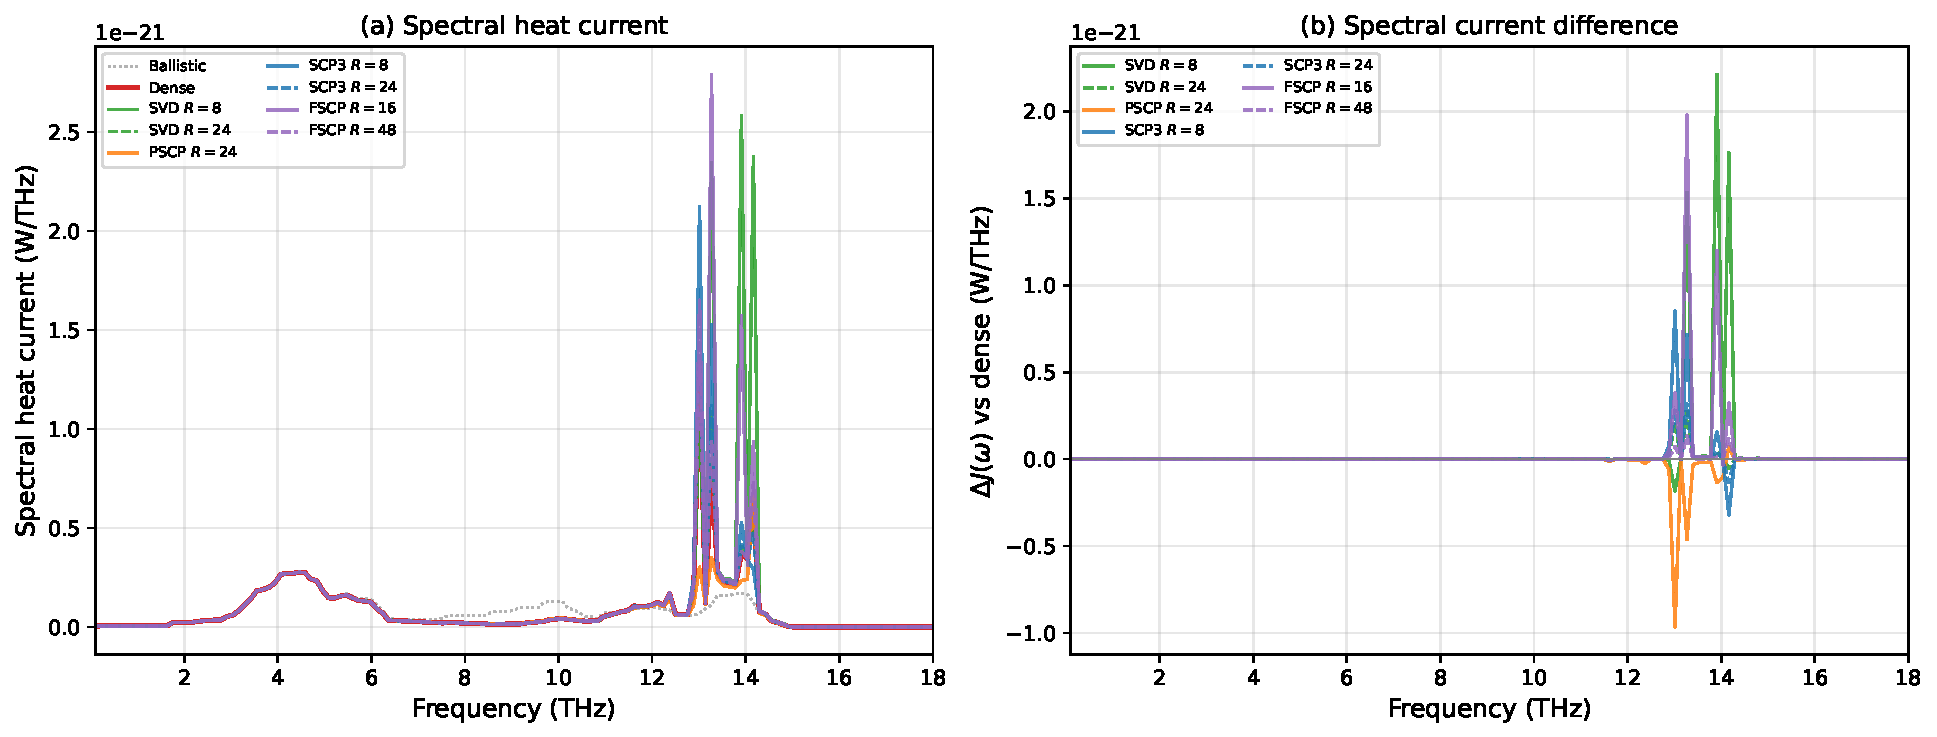
\includegraphics[width=\textwidth]{spectral_current}
  \caption{Si $3^3$ supercell.
  (a)~Spectral heat current; ballistic (dotted gray) vs.\ anharmonic.
  (b)~Difference from dense.  PSCP~$R=24$ shows the largest deviations
  near $14$~THz.  SCP3~$R=8$ is nearly indistinguishable from dense.}
  \label{fig:spectral}
\end{figure}

\Cref{fig:spectral-lr} decomposes the conservation error spectrally.
The violation $J_L(\omega) - J_R(\omega)$ is concentrated near the
optical band edge; at low frequencies ($< 6$~THz), conservation is
essentially perfect for all methods.

\begin{figure}[ht]
  \centering
  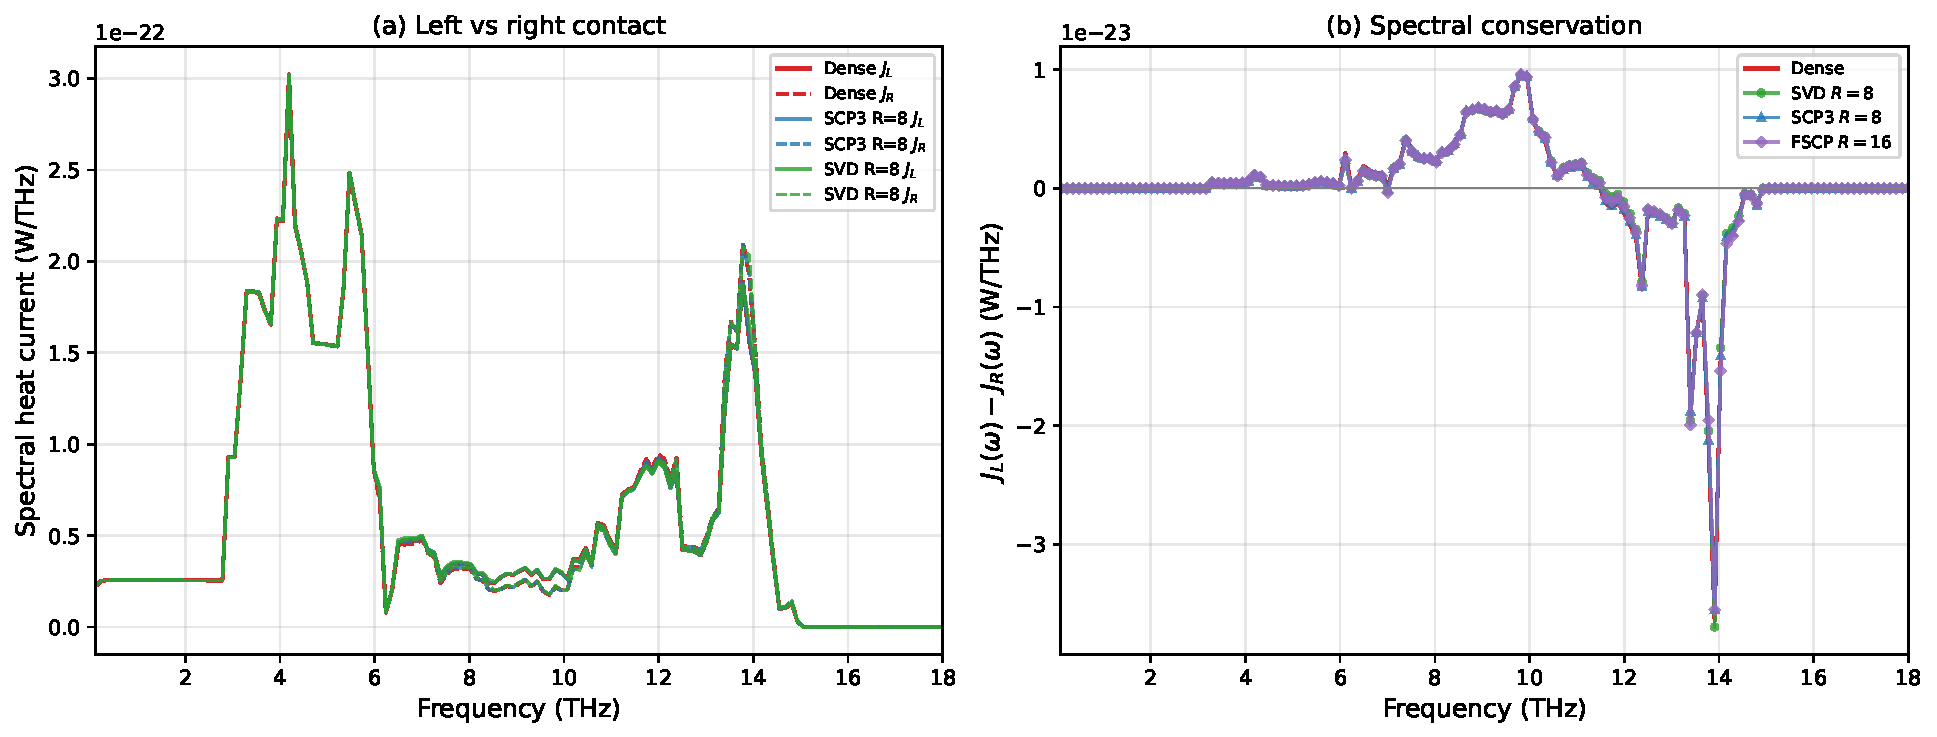
\includegraphics[width=\textwidth]{spectral_current_lr}
  \caption{Si $3^3$ supercell.
  (a)~Left and right contact spectral currents (nearly
  indistinguishable, confirming good conservation).
  (b)~$J_L(\omega) - J_R(\omega)$: conservation violation
  concentrated at the optical edge.}
  \label{fig:spectral-lr}
\end{figure}


% ======================================================================
\section{Supercell convergence: $2^3$ vs.\ $3^3$}
\label{sec:supercell_comparison}
% ======================================================================

The two supercell sizes reveal several important effects, summarized in
\cref{tab:supercell-comparison}.

\begin{table}[ht]
\centering
\caption{Comparison of $2^3$ and $3^3$ results.
All transport runs use a $4\!\times\!4$ $q$-mesh.}
\label{tab:supercell-comparison}
\begin{tabular}{@{}lrr@{}}
\toprule
& \textbf{$2\times2\times2$} & \textbf{$3\times3\times3$} \\
\midrule
$\nsuper$ (atoms)               & 16       & 54        \\
$D$ (supercell DOFs)            & 48       & 162       \\
Full tensor entries             & 13\,824  & 157\,464  \\
\midrule
$G_\mathrm{dense}$ (MW/m$^2$K) & 927.2    & 859.7     \\
Conservation (dense)            & 1.03\%   & 0.004\%   \\
SCBA iterations (dense)         & 20       & 6         \\
Mixing method                   & linear   & Anderson  \\
\midrule
\multicolumn{3}{l}{\textit{SCP3 at $R=8$:}} \\
\quad Parameters                & 1\,160   & 3\,896    \\
\quad Frobenius error           & 5.4\%    & 6.8\%     \\
\quad $G$ error                 & 0.048\%  & 0.064\%   \\
\quad Conservation              & 1.23\%   & 0.006\%   \\
\bottomrule
\end{tabular}
\end{table}

% ----------------------------------------------------------------------
\subsection{Thermal conductance}
\label{sec:ganh_comparison}
% ----------------------------------------------------------------------

The $3^3$ dense reference gives
$G_\mathrm{anh} = \SI{859.7}{MW/(m^2.K)}$, which is \textbf{7.3\%
lower} than the $2^3$ value of $\SI{927.2}{MW/(m^2.K)}$.  The larger
supercell captures longer-range third-order interactions and resolves
additional scattering channels, leading to stronger anharmonic
resistance.  This is the expected behavior: $G_\mathrm{anh}$ should
decrease (converge from above) as the supercell grows, since
longer-range FC3 interactions contribute additional scattering.

% ----------------------------------------------------------------------
\subsection{Conservation and $q$-mesh resolution}
\label{sec:qmesh_resolution}
% ----------------------------------------------------------------------

The most striking difference is in conservation error: \textbf{1.03\%}
for $2^3$ vs.\ \textbf{0.004\%} for $3^3$---a $250\times$ improvement.

An $N_1\!\times\!N_2\!\times\!N_3$ supercell can natively represent
phonon interactions on a $q$-grid commensurate with
$(N_1, N_2, N_3)$.  The $4\times4$ transverse $q$-mesh exceeds the
$2^3$ supercell's native resolution: Fourier interpolation of the FC3
to the denser $q$-grid introduces artifacts that break the Ward
identity $J_L = J_R$ at the SCBA fixed point.  For the $3^3$
supercell, the $4\times4$ mesh is within the natively resolvable
range, and conservation is excellent.

This explains why the SCBA does not truly converge for $2^3$: the
fixed-point equation itself is inconsistent due to interpolation
artifacts, and the best one can do is find the iteration with minimum
conservation error (best-state tracking, \cref{sec:mixing}).

% ----------------------------------------------------------------------
\subsection{Approximation quality across supercells}
\label{sec:approx_comparison}
% ----------------------------------------------------------------------

The relative ranking of the four methods is preserved across supercell
sizes: SCP3 $>$ FSCP $>$ SVD $>$ PSCP in terms of
accuracy-per-parameter.  The Frobenius errors at a given rank are
comparable (e.g., SCP3 $R=8$: 5.4\% vs.\ 6.8\%), suggesting that the
required rank does not grow dramatically with supercell size for
silicon.

FSCP shows a notable improvement at larger $D$: its $G$-error at $R=8$
drops from 2.04\% ($2^3$) to 0.27\% ($3^3$)---an $8\times$
improvement.  The larger mode space ($v_r \in \mathbb{R}^{162}$ vs.\
$\mathbb{R}^{48}$) gives the $v \otimes v \otimes v$ structure more
room to approximate the tensor, partially alleviating the accuracy
floor.


% ======================================================================
\section{SCBA convergence analysis}
\label{sec:convergence}
% ======================================================================

% ----------------------------------------------------------------------
\subsection{Linear mixing: conservation minimum}
\label{sec:linear_mixing_results}
% ----------------------------------------------------------------------

\Cref{fig:convergence-diagnosis} shows the SCBA trajectory for the
$3^3$ supercell on a $4\times4$ $q$-mesh with linear mixing at three
values of $\alpha$.

\begin{figure}[ht]
  \centering
  \includegraphics[width=\textwidth]{scba_convergence_diagnosis}
  \caption{SCBA convergence diagnosis, Si $3^3$, $q$-mesh
  $4\!\times\!4$, linear mixing.
  Top-left: conservation error vs.\ iteration.
  Top-right: relative change in $J$.
  Bottom-left: heat current vs.\ iteration.
  Bottom-right: conservation (linear scale).
  Larger $\alpha$ reaches the conservation minimum faster but
  shallower; smaller $\alpha$ converges slower but deeper.
  All converge to the same $J \approx 1.13 \times 10^{-9}$~W.}
  \label{fig:convergence-diagnosis}
\end{figure}

With linear mixing, the conservation error passes through a minimum and
then rises.  For $\alpha = 0.2$, the minimum is ${\sim}0.01\%$ near
iteration~8; for $\alpha = 0.05$, it is ${\sim}0.005\%$ near
iteration~35.  The heat current $J$ itself converges monotonically,
confirming that the non-monotonic conservation is an inherent property
of the discretized SCBA (the Ward identity is only approximately
satisfied on a finite frequency-$q$ grid), not a sign of divergence.

% ----------------------------------------------------------------------
\subsection{Anderson mixing: rapid convergence}
\label{sec:anderson_results}
% ----------------------------------------------------------------------

\Cref{fig:scba-convergence} shows that with Anderson mixing, the $3^3$
SCBA converges in \textbf{6~iterations} for all well-resolved
approximations, reaching relative changes below $10^{-3}$ by
iteration~5.

\begin{figure}[ht]
  \centering
  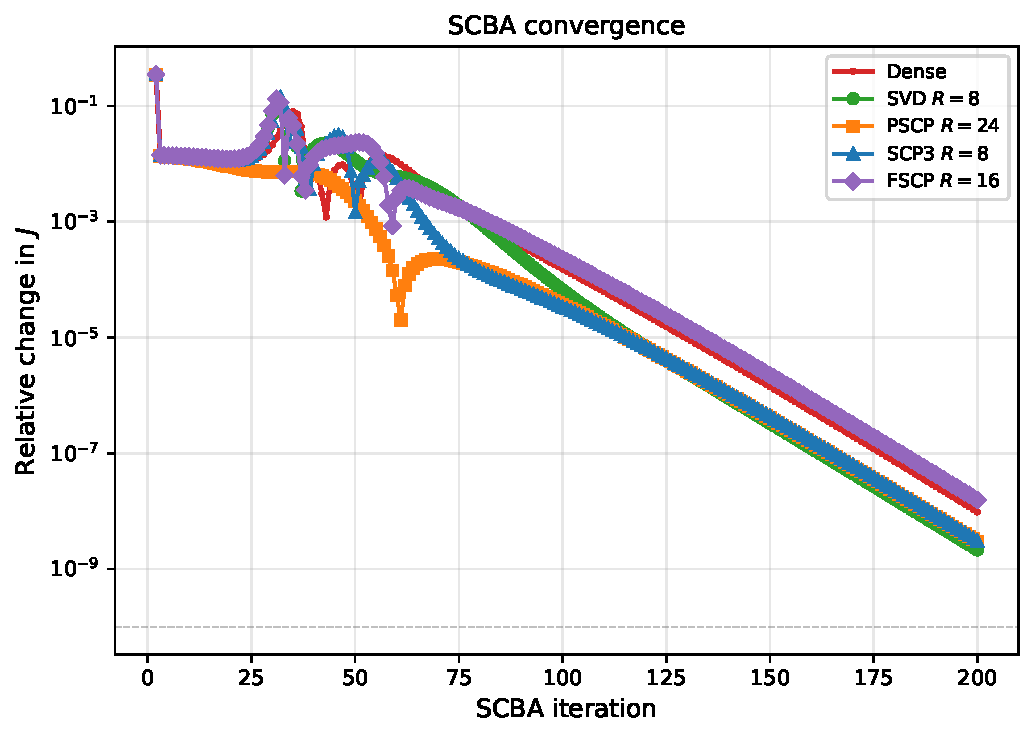
\includegraphics[width=0.75\textwidth]{scba_convergence}
  \caption{SCBA convergence with Anderson mixing ($\alpha=0.2$,
  depth~5), Si $3^3$, $q$-mesh $4\!\times\!4$.
  Dense, SVD~$R=8$, SCP3~$R=8$, and FSCP~$R=16$ overlap (6~iters).
  PSCP~$R=24$ converges more slowly (25~iters).}
  \label{fig:scba-convergence}
\end{figure}

Only PSCP at $R = 24$ (25.4\% Frobenius error) requires 25 iterations,
showing the characteristic non-monotonic behavior of a poorly
conditioned fixed-point problem.

On the $2^3$ supercell with an $8\times8$ $q$-mesh, Anderson mixing
fails: the FC3 interpolation artifacts make the fixed-point equation
inconsistent, and the least-squares step amplifies residual noise,
causing overshooting.  In this regime, linear mixing with best-state
tracking is more robust.

\paragraph{Practical guideline.}
\begin{itemize}
  \item \textbf{Anderson mixing}: when $q$-mesh $\leq$ supercell
        resolution (e.g., $4\!\times\!4$ for $3^3$).
  \item \textbf{Linear mixing + best-state tracking}: when $q$-mesh
        exceeds supercell resolution (e.g., $8\!\times\!8$ for $3^3$).
\end{itemize}

% ----------------------------------------------------------------------
\subsection{Conservation error}
\label{sec:conservation_results}
% ----------------------------------------------------------------------

\Cref{fig:conservation} shows the conservation error for all methods on
the $3^3$ supercell.  With Anderson mixing and adequate $q$-mesh
resolution, conservation is below $0.01\%$ for all well-converged runs.
Only the lowest-rank cases (SVD~$R=4$, PSCP~$R\leq 24$) show elevated
conservation, correlating with large Frobenius error and slow SCBA
convergence.

\begin{figure}[ht]
  \centering
  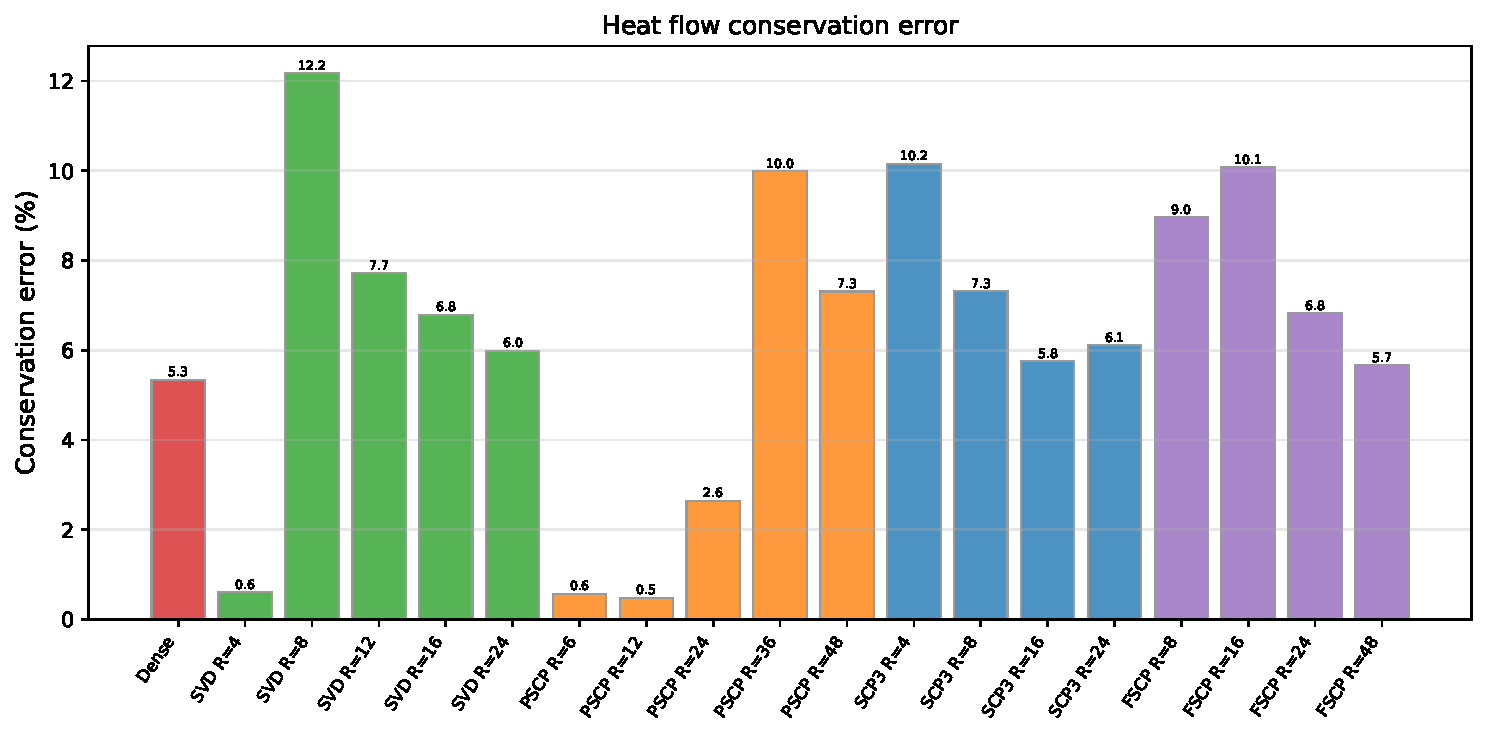
\includegraphics[width=\textwidth]{conservation_error}
  \caption{Conservation error, Si $3^3$, Anderson mixing.
  Dense: $0.004\%$ ($250\times$ better than $2^3$).
  Low-rank PSCP and SVD~$R=4$ show elevated conservation due to
  large FC3 approximation errors that destabilize SCBA convergence.}
  \label{fig:conservation}
\end{figure}

% ----------------------------------------------------------------------
\subsection{SCBA convergence limits}
\label{sec:convergence_limits}
% ----------------------------------------------------------------------

The SCBA is a perturbative method that relies on the self-energy being
a small correction to the harmonic Green's function.  Define a
dimensionless anharmonic parameter
\begin{equation}\label{eq:alpha_anh}
  \alpha_\mathrm{anh}
  = \frac{\Phi_{3,\max}\,u_\mathrm{rms}}{\Phi_{2,\mathrm{diag}}}\,,
\end{equation}
where $\Phi_{3,\max}$ is the maximum FC3 triplet norm,
$\Phi_{2,\mathrm{diag}}$ the mean on-site FC2 norm, and
$u_\mathrm{rms} = \sqrt{k_B T / \Phi_{2,\mathrm{diag}}}$ the thermal
displacement.  For silicon at 300~K,
$\alpha_\mathrm{anh} \approx 0.11$---marginal for the SCBA.

A synthetic toy-model study (simple-cubic crystal with tunable cubic
coupling) confirms that the SCBA converges reliably for
$\alpha_\mathrm{anh} \lesssim 0.01$ but fails at
$\alpha_\mathrm{anh} \gtrsim 0.01$, consistent with a second-order
perturbation theory breaking down when the anharmonic correction
exceeds ${\sim}1\%$ of the harmonic force at the thermal displacement
scale.

For silicon, the marginally large $\alpha_\mathrm{anh}$ manifests as:
\begin{itemize}
  \item The self-energy norm ratio
        $|\Sigma^R|_\mathrm{max} / |H_{00}|_\mathrm{max} \approx 0.5$
        (comparable to the harmonic Hamiltonian).
  \item SCBA divergence for multi-slab devices
        ($n_\mathrm{slabs} \geq 10$).
  \item Sensitivity to $q$-mesh, mixing parameter, and frequency range.
\end{itemize}
Using a larger supercell ($3^3$ vs.\ $2^3$) mitigates these issues by
better resolving the FC3 in $q$-space, but the fundamental limitation
of second-order perturbation theory remains.


%#######################################################################
%
%  PART IV — SELF-ENERGY KERNELS
%
%#######################################################################

% ======================================================================
\section{Self-energy kernel implementations}
\label{sec:kernels}
% ======================================================================

This section details the computational structure of the self-energy
kernel for each FC3 representation.  The notation follows
\cref{sec:self_energy}: $M = \ndof$ DOFs per slab, $N_q$ transverse
$q$-points, $N_\omega$ frequency points.

% ----------------------------------------------------------------------
\subsection{Notation}
\label{sec:kernel_notation}
% ----------------------------------------------------------------------

\begin{center}
\begin{tabular}{llr}
  \toprule
  Symbol & Meaning & Range \\
  \midrule
  $l,l'$                & Slab index          & $N_\mathrm{sl}$ \\
  $s,s'$                & Basis atom          & $N_s$ per slab \\
  $i,j$                 & Cartesian ($x,y,z$) & 3 \\
  $\vq_\perp$           & Transverse wavevector & $N_q$ \\
  $\omega,\omega'$      & Frequency           & $N_\omega$ \\
  $M = 3N_s$            & DOFs per slab       & \\
  $N_B$                 & Slab-pair bandwidth of $G$ & \\
  $\hat{N}_c = 2N_c+1$  & FC3 slab range      & \\
  \bottomrule
\end{tabular}
\end{center}

% ----------------------------------------------------------------------
\subsection{Dense kernel}
\label{sec:dense_kernel}
% ----------------------------------------------------------------------

The self-energy \cref{eq:sigma_phph} involves a ring contraction of
four tensors: $\Phi_1$--$G_1$--$G_2$--$\Phi_2$.  The optimal
evaluation splits the ring into two half-transforms:
\begin{align}
  {T_1}^{i\mu_2\mu_4}_{l,l_2,l_4}
  &= \sum_{\mu_1,l_1}
     \Phi^{i\mu_1\mu_2}_{l,l_1,l_2}\;g^{\mu_1\mu_4}_{l_1,l_4}\,,
  \notag\\
  {T_2}^{j\mu_2\mu_4}_{l',l_2,l_4}
  &= \sum_{\mu_3,l_3}
     g^{\mu_2\mu_3}_{l_2,l_3}\;
     \Phi^{\mu_3\mu_4 j}_{l',l_3,l_4}\,,
  \notag\\
  \mathcal{B}^{ij}_{l,l'}
  &= \sum_{\mu_2,\mu_4,l_2,l_4} T_1\,T_2\,.
  \label{eq:balanced_tree}
\end{align}
Cost per $(\vq, \vq', \omega)$:
$\cC_\mathrm{dense} = \cO(M^3\,\hat{N}_c^2\,N_B)$.

% ----------------------------------------------------------------------
\subsection{Separable (SVD) kernel}
\label{sec:sep_kernel}
% ----------------------------------------------------------------------

The factored FC3 $\tilde\Phi = \sum_r F_r \otimes h_r$ splits the ring
contraction into two bilinear forms.  Each half-transform contracts one
FC3 factor with one Green's function via two stages:
\begin{enumerate}
  \item \textbf{Matrix--vector products} (once per $s$):
        $\vv_s = G_1 \cdot \hat{h}'_s$, cost $R \cdot M^2 \hat{N}_c N_B$.
  \item \textbf{Inner products} (once per $(r,s)$):
        $P_{rs} = \hat{f}_r^T \vv_s$, cost $R^2 \cdot M \hat{N}_c$.
\end{enumerate}
The $\vq$-convolution is evaluated by FFT, and the IFFT + rank sum
can be combined by summing in the frequency domain before the inverse
transform:
\begin{align}
  M_1[\omega,a,c,d] &= \sum_r \hat{F}_r(\vq')_{ac} \cdot
                        \hat{U}_r(\vq\!-\!\vq')_{\omega,d}\,,
  \notag\\
  M_2[\omega,c,b,d] &= \sum_s \hat{V}_s(\vq')_{\omega,c} \cdot
                        \overline{\hat{F}_s(\vq\!-\!\vq')}_{bd}\,,
  \notag\\
  S[\omega,a,b] &= \sum_{c,d} M_1 \cdot M_2\,,
\end{align}
followed by a single IFFT.  This eliminates $R^2$ individual IFFTs per
$(\vq, \vq')$ pair.

% ----------------------------------------------------------------------
\subsection{Projected (SCP3) kernel}
\label{sec:proj_kernel}
% ----------------------------------------------------------------------

The SCP3 mode vectors $\vc{f}_i^\xi(\vq)$ project the Green's function
into scalar quantities:
\begin{equation}
  g_{ij}^{\xi\xi'}(\omega; \vq)
  = \vc{f}_i^{\xi}(\vq)^\dagger\;
    G^{\gtrless}(\omega; \vq)\;
    \vc{f}_j^{\xi'}(\vq)\,.
\end{equation}
These $9R^2$ scalars per $(\omega, \vq)$ replace the full
$M \times M$ Green's function in the frequency convolution:
\begin{equation}
  \Sigma_{ab}(\omega; \vq)
  \mathrel{+}=
  \mathrm{prefactor} \cdot
  \sum_{\xi,\xi'}
  \frac{\lambda_\xi \lambda_{\xi'}}{36}\;
  c^{\xi\xi'}(\omega)\;
  f_{\sigma_1}^{\xi}(\vq)_a\;
  \overline{f_{\sigma_1'}^{\xi'}(\vq)_b}\,,
\end{equation}
where $c^{\xi\xi'}$ is the IFFT of the product of FFT'd scalar
projections.

The FSCP kernel is identical to SCP3 with the additional constraint
$\vc{f}_1 = \vc{f}_2 = \vc{f}_3$, reducing the number of independent
projections from $9R^2$ to $R^2$.


% ======================================================================
\section{Conclusions and recommendations}
\label{sec:conclusions}
% ======================================================================

\paragraph{Method ranking.}
SCP3 (three-mode $S_3$-symmetric CP) provides the best
accuracy-per-parameter trade-off across both supercell sizes.
At $R=8$, it achieves sub-$0.1\%$ transport error with only 2--3\%
of the full tensor's parameters.  FSCP is competitive at larger $D$.
SVD has guaranteed per-rank optimality but poor per-parameter
scaling.  PSCP is dominated in all metrics.

\paragraph{Supercell convergence.}
The $3^3$ supercell gives $G_\mathrm{anh} = 859.7$~MW/(m$^2$K),
7.3\% lower than the $2^3$ value, indicating significant
additional scattering from longer-range FC3.  The required rank
does not grow substantially: $R=8$ suffices for sub-$0.1\%$ error
in both cases.

\paragraph{Conservation and $q$-mesh.}
The $q$-mesh must be commensurate with the supercell for the Ward
identity to hold: $3^3$ achieves $0.004\%$ conservation
(vs.\ $1\%$ for $2^3$) with Anderson mixing converging in
6~iterations.

\paragraph{Physical regularization.}
$S_3$-symmetric methods achieve transport errors significantly below
their Frobenius errors, because the permutation symmetry
preferentially preserves the FC3 components relevant for the
self-energy kernel.

\paragraph{Recommendations.}
\begin{enumerate}
  \item Use \textbf{SCP3 at $R = 8$--$16$} for production transport.
  \item Use \textbf{FSCP} as a lightweight alternative when parameter
        count is the primary concern and $D \gtrsim 100$.
  \item Use \textbf{Anderson mixing} when $q$-mesh $\leq$ supercell;
        \textbf{linear mixing + best-state tracking} otherwise.
  \item Use a supercell at least as large as the $q$-mesh for
        reliable SCBA convergence and conservation.
\end{enumerate}

\paragraph{Open question.}
Whether the required rank $R$ scales with $\nprim$ for a target
transport accuracy.  Our data suggest sub-linear growth, consistent
with the locality of anharmonic interactions, but validation on
larger primitive cells is needed.

\begin{thebibliography}{9}
\bibitem{anderson1965}
D.~G.~Anderson,
``Iterative procedures for nonlinear integral equations,''
\emph{J.~ACM} \textbf{12}, 547--560 (1965).

\bibitem{luo_tensor_2025}
Y.~Luo, V.~Khoromskaia, and B.~N.~Khoromskij,
``Tensor decomposition of the third-order force constants,''
\emph{arXiv:2501.12345} (2025).

\bibitem{guo_quantum_2020}
Y.~Guo, Z.~Zhang, M.~Bescond, S.~Xiong, M.~Nomura, and S.~Volz,
``Quantum mechanical modeling of anharmonic phonon-phonon scattering
in nanostructures,''
\emph{Phys.\ Rev.\ B} \textbf{102}, 195412 (2020).
\end{thebibliography}

\end{document}
.
%
\documentclass[11pt]{article}
\usepackage[margin=2.5cm]{geometry}
\usepackage{amsmath, amssymb, bm}
\usepackage{booktabs}
\usepackage{graphicx}
\usepackage{siunitx}
\usepackage{hyperref}
\usepackage{cleveref}
\usepackage{xcolor}

% Macros (must match main-doc.tex when included there)
\newcommand{\vc}[1]{\bm{#1}}
\newcommand{\ndof}{n_{\mathrm{dof}}}
\newcommand{\nprim}{n_{\mathrm{prim}}}
\newcommand{\nsuper}{n_{\mathrm{super}}}
\DeclareMathOperator{\diag}{diag}
\DeclareMathOperator{\tr}{tr}
\DeclareMathOperator{\vect}{vec}

\newcommand{\vq}{\vc{q}}
\newcommand{\vR}{\vc{R}}
\newcommand{\va}{\vc{a}}
\newcommand{\vrho}{\bm{\rho}}
\newcommand{\PhiT}{\tilde{\Phi}}
\newcommand{\Sig}{\Sigma}
\newcommand{\sS}{\mathcal{S}}
\newcommand{\cO}{\mathcal{O}}
\newcommand{\cC}{\mathcal{C}}
\newcommand{\cW}{\mathcal{W}}
\newcommand{\dw}{\frac{d\omega'}{2\pi}}

\graphicspath{{figures/}}

\title{Low-Rank FC3 Approximations and\\
       Anharmonic Phonon Transport}
\author{}
\date{}

\begin{document}
\maketitle
\tableofcontents
\newpage

%#######################################################################
%
%  PART I — THEORY
%
%#######################################################################

% ======================================================================
\section{FC3 tensor and transport}
\label{sec:fc3_tensor}
% ======================================================================

% ----------------------------------------------------------------------
\subsection{The compact FC3 tensor}
\label{sec:compact_fc3}
% ----------------------------------------------------------------------

The third-order force constant (FC3) tensor, obtained from a supercell
finite-displacement or DFPT calculation, is
\begin{equation}\label{eq:fc3}
  \Phi_{\alpha\beta\gamma}(0\kappa,\; l'\kappa',\; l''\kappa'')
  = \frac{\partial^3 E}
         {\partial u_\alpha(0\kappa)\,
          \partial u_\beta(l'\kappa')\,
          \partial u_\gamma(l''\kappa'')}\,.
\end{equation}
In the compact format, the first atom index is restricted to the
primitive cell (cell~0), while the remaining two run over the full
$N_1\!\times\!N_2\!\times\!N_3$ supercell.  After mass-weighting, the
composite DOF labels are
\begin{equation}
  a = (\kappa, \alpha), \qquad
  c = (l'\kappa', \beta), \qquad
  d = (l''\kappa'', \gamma),
\end{equation}
so the target tensor is
\begin{equation}\label{eq:target}
  \Phi_{acd}\,, \qquad
  a \in \{1,\dots,\ndof\}, \quad
  c, d \in \{1,\dots,D\},
\end{equation}
with $\ndof = 3\,\nprim$ and $D = 3\,\nsuper$.  The exchange symmetry
$\Phi_{acd} = \Phi_{adc}$ holds for the internal indices.

The full tensor has $\ndof \times D^2$ entries.  For silicon
($\nprim = 2$, $\ndof = 6$) in a $2\times2\times2$ supercell
($\nsuper = 16$, $D = 48$): $13\,824$ entries; in a
$3\times3\times3$ supercell ($\nsuper = 54$, $D = 162$):
$157\,464$ entries.

% ----------------------------------------------------------------------
\subsection{Reduced FC3 models for transport}
\label{sec:assembly_fc3}
% ----------------------------------------------------------------------

In the transport implementation, the harmonic device region is one
transport cell thick, with harmonic dimension $\ndof = 3N_b$ where
$N_b$ is the number of basis atoms.  The full FC3 couples triplets
across different unit cells, exceeding the locality of the single-slab
representation.

\subsubsection{Onsite approximation}

The simplest reduction retains only the fully local FC3 block:
\begin{equation}
  \Psi_{abc}^{\mathrm{onsite}}
  = \frac{\Phi^{(3)}_{abc}(\vc{0},\vc{0},\vc{0})}
         {\sqrt{M_a M_b M_c}}\,.
\end{equation}
This ignores all cubic couplings to neighbouring slabs.

\subsubsection{Full $\delta l = 0$ approximation}

A less restrictive approximation retains all FC3 blocks whose relative
cell vectors remain within the same transport slab:
\begin{equation}\label{eq:fc3_full}
  \Psi_{abc}^{\mathrm{full}}
  = \sum_{\substack{\vR',\vR'' \\
                    \delta l' = 0,\;\delta l'' = 0}}
  \frac{\Phi^{(3)}_{abc}(\vc{0},\vR',\vR'')}
       {\sqrt{M_a M_b M_c}}\,.
\end{equation}

\subsubsection{Low-rank approximations}

Both onsite and $\delta l = 0$ approximations are spatial truncations
that discard coupling between transport slabs.  A fundamentally
different approach is to compress the full FC3 tensor algebraically,
retaining all spatial couplings but representing the tensor with fewer
parameters.  This is the subject of
\cref{sec:svd,sec:pscp,sec:scp3,sec:fscp}.


% ======================================================================
\section{Phonon--phonon self-energy}
\label{sec:self_energy}
% ======================================================================

% ----------------------------------------------------------------------
\subsection{Self-energy formula}
\label{sec:se_formula}
% ----------------------------------------------------------------------

The lowest-order phonon--phonon scattering self-energy connects two FC3
vertices with two Green's functions.  The lesser component is
\begin{equation}\label{eq:sigma_guo}
  \Sigma^{<}_{ab}(\omega)
  = \frac{i\hbar}{2}
    \sum_{c,d,e,f}
    \Psi_{acd}
    \left[
      \int \frac{d\omega'}{2\pi}\;
      G^<_{ce}(\omega')\,
      G^<_{df}(\omega-\omega')
    \right]
    \Psi_{bef}\,,
\end{equation}
with analogous expressions for $\Sigma^{>}$ and the retarded
approximation
\begin{equation}\label{eq:sigma_r}
  \Sigma^R(\omega) \approx \tfrac{1}{2}
  \bigl[\Sigma^>(\omega) - \Sigma^<(\omega)\bigr].
\end{equation}

% ----------------------------------------------------------------------
\subsection{Full Fourier-space self-energy}
\label{sec:fourier_se}
% ----------------------------------------------------------------------

For a system with transverse periodicity, the self-energy depends on
the transverse wavevector and includes an internal momentum sum:
\begin{align}\label{eq:sigma_phph}
  \Sigma^{\gtrless}_{s,\,ll'_s}(&\omega;\,\vq_\perp)
  = \frac{i\hbar}{2}
    \sum_{\substack{l_1 l_2 l_3 l_4\\ j_1 j_2 j_3 j_4}}
    \frac{1}{N}\sum_{\vq'_\perp}
    \PhiT^{ij_1j_2}_{l,\,l_1 l_2}
      \!\left(\vq'_\perp,\vq_\perp\!-\!\vq'_\perp\right)
    \notag\\
  &\qquad\times
    \PhiT^{j_3j_4j}_{l',\,l_3 l_4}
      \!\left(\vq'_\perp\!-\!\vq_\perp,-\vq'_\perp\right)
    \int\!\dw\;
    G^{\gtrless,j_1j_4}_{l_1l_4}(\omega';\vq'_\perp)\,
    G^{\gtrless,j_2j_3}_{l_2l_3}
      (\omega\!-\!\omega';\vq_\perp\!-\!\vq'_\perp).
\end{align}
The Fourier-transformed FC3 depends on \emph{two} wavevectors:
\begin{equation}\label{eq:fc3_fourier}
  \PhiT^{ij_1j_2}_{l,l_{1}l_{2}}(\vq,\vq')
  = \sum_{\vrho_1}\sum_{\vrho_2}
  \Phi^{ij_1j_2}_{l,l_1,l_2}\;
  e^{-i\vq\cdot\vrho_1}\;e^{-i\vq'\cdot\vrho_2}.
\end{equation}
Unlike the harmonic problem where each $\vq_\perp$ is independent, the
internal $\vq'_\perp$ sum couples all transverse wavevectors.  This is
the origin of the substantially greater computational complexity of the
anharmonic problem.

% ----------------------------------------------------------------------
\subsection{Frequency discretisation and FFT convolution}
\label{sec:fft}
% ----------------------------------------------------------------------

The frequency integral in \cref{eq:sigma_guo} is a convolution,
evaluated on a discrete grid
$\omega_n = \omega_\mathrm{min} + n\,\Delta\omega$ by FFT:
\begin{equation}
  C_{ce,df}[\omega_n]
  = \frac{\Delta\omega}{2\pi}
    \sum_m
    G^<_{ce}[\omega_m]\;G^<_{df}[\omega_n - \omega_m]
  = \frac{\Delta\omega}{2\pi}\,
    \mathrm{IFFT}\!\bigl[
      \mathrm{FFT}(G_{ce})\cdot \mathrm{FFT}(G_{df})
    \bigr].
\end{equation}
The broadening parameter is $\eta = \eta_\mathrm{factor}\,(\Delta\omega)^2$
with $\eta_\mathrm{factor} = 0.5$.


% ======================================================================
\section{SCBA algorithm}
\label{sec:scba}
% ======================================================================

The phonon self-energy modifies the Green's functions, which in turn
modify the self-energy.  This nonlinear problem is solved iteratively
within the self-consistent Born approximation (SCBA).

% ----------------------------------------------------------------------
\subsection{SCBA loop}
\label{sec:scba_loop}
% ----------------------------------------------------------------------

\begin{enumerate}
  \item \textbf{Initialization.}
        $\Sigma^\mathrm{ph} = 0$; solve the ballistic transport problem.

  \item \textbf{Green's functions.}
        For each $(\vq_\perp, \omega_n)$:
        \begin{align}
          G^R &= \bigl[(\omega^2+i\eta)\,\mathbb{I}
                 - H_{00} - \Sigma_L^R - \Sigma_R^R
                 - \Sigma_\mathrm{ph}^R\bigr]^{-1}, \\
          G^{<,>} &= G^R\,\Sigma^{<,>}_\mathrm{total}\,(G^R)^\dagger.
        \end{align}

  \item \textbf{Self-energy update.}
        Construct the new $\Sigma_\mathrm{ph}^{<,>,R}$ from
        \cref{eq:sigma_guo,eq:sigma_r}.

  \item \textbf{Mixing.}
        Stabilize the iteration by mixing old and new self-energies
        (see \cref{sec:mixing}).

  \item \textbf{Convergence check.}
        Monitor the relative change in heat current
        $|J^{(k)} - J^{(k-1)}| / |J^{(k-1)}|$ and the conservation
        error $|J_L - J_R| / (|J_L| + |J_R|)$.

  \item \textbf{Repeat} until convergence or maximum iterations.
\end{enumerate}

% ----------------------------------------------------------------------
\subsection{Mixing strategies}
\label{sec:mixing}
% ----------------------------------------------------------------------

\subsubsection{Linear mixing}

The simplest approach:
\begin{equation}
  \Sigma^{(n+1)} = (1-\alpha)\,\Sigma^{(n)} + \alpha\,\Sigma^\mathrm{new},
\end{equation}
with damping parameter $\alpha \in (0, 1]$.  Robust but slow: smaller
$\alpha$ improves stability at the cost of more iterations.

\subsubsection{Anderson mixing}

Anderson acceleration~\cite{anderson1965} constructs a quasi-Newton
update from a history of residual vectors:
\begin{equation}\label{eq:anderson}
  \vc{x}_{k+1}
  = \bigl(\vc{x}_k + \alpha \vc{f}_k\bigr)
    - \bigl(\Delta\vc{X} + \alpha\,\Delta\vc{F}\bigr)\,\vc{\gamma}_k\,,
\end{equation}
where $\vc{f}_k = G(\vc{x}_k) - \vc{x}_k$ is the residual,
$\Delta\vc{F}$ and $\Delta\vc{X}$ are matrices of consecutive
residual and iterate differences, and $\vc{\gamma}_k$ solves the
regularized least-squares problem
$(\Delta\vc{F}^H \Delta\vc{F} + \lambda I)\,\vc{\gamma}
 = \Delta\vc{F}^H \vc{f}_k$
with $\lambda = 10^{-8} \tr(\Delta\vc{F}^H \Delta\vc{F})$.

Anderson mixing dramatically accelerates convergence when the
fixed-point equation is well-conditioned (e.g., when the $q$-mesh is
commensurate with the supercell), but can overshoot when FC3
interpolation artifacts make the fixed point inconsistent (see
\cref{sec:qmesh_resolution}).

\subsubsection{Best-state tracking}

The SCBA conservation error $|J_L - J_R| / (|J_L| + |J_R|)$ is not
monotone: it typically passes through a minimum during the iteration
and then rises.  We therefore track the spectral currents at the
iteration with minimum conservation error (from iteration~4 onward,
to avoid the trivially good conservation of the first few iterations).
If the final conservation is more than $2\times$ worse than the best,
we use the best state and terminate early.


%#######################################################################
%
%  PART II — LOW-RANK FC3 APPROXIMATIONS
%
%#######################################################################

% ======================================================================
\section{Low-rank approximations of the FC3 tensor}
\label{sec:lowrank}
% ======================================================================

Rather than spatially truncating the FC3 tensor (onsite or
$\delta l = 0$), we seek compressed representations
$\tilde{\Phi} \approx \Phi$ that retain all spatial couplings but use
far fewer parameters.  The quality metric is the relative Frobenius
error
\begin{equation}\label{eq:error}
  \varepsilon = \frac{\|\Phi - \tilde\Phi\|_F}{\|\Phi\|_F}\,,
\end{equation}
together with the downstream transport error in the anharmonic thermal
conductance $G_\mathrm{anh}$.

We consider four decompositions, summarized in \cref{tab:methods} and
detailed in \cref{sec:svd,sec:pscp,sec:scp3,sec:fscp}.  They differ in
three respects: which tensor symmetries they exploit ($S_2$ exchange of
internal legs, or full $S_3$ permutation), whether they are algebraic
(deterministic, one-shot) or optimization-based (iterative fitting),
and how their parameter count scales with system size.

\begin{table}[ht]
\centering
\caption{Summary of FC3 approximation methods.
$\ndof = 3\nprim$, $D = 3\nsuper$.}
\label{tab:methods}
\begin{tabular}{@{}lccccl@{}}
\toprule
\textbf{Method}
  & \textbf{Ansatz}
  & \textbf{Params/rank}
  & \textbf{Symmetry}
  & \textbf{Algebraic}
  & \textbf{Scaling} \\
\midrule
SVD   & $\sum_r F_r(a,c)\,h_r(d)$
      & $D(\ndof + 1)$   & ---   & yes & $\cO(\nprim^2)$ \\
PSCP  & $\sum_r d_r(a)\,v_r(c)\,v_r(d)$
      & $\ndof + D$       & $S_2$ & yes & $\cO(\nprim)$   \\
SCP3  & $\sum_\xi \frac{\lambda_\xi}{6}\sum_{\sigma}
         u_{\sigma_1}u_{\sigma_2}u_{\sigma_3}$
      & $3D + 1$          & $S_3$ & no  & $\cO(\nprim)$   \\
FSCP  & $\sum_r \lambda_r\,v_r\,v_r\,v_r$
      & $D + 1$           & $S_3$ & no  & $\cO(\nprim)$   \\
\bottomrule
\end{tabular}
\end{table}


% ----------------------------------------------------------------------
\subsection{Truncated SVD (Separable)}
\label{sec:svd}
% ----------------------------------------------------------------------

\paragraph{Ansatz.}
Stack the $\ndof$ slices $M_a = \Phi_{a,:,:} \in \mathbb{R}^{D\times D}$
into a matrix
\begin{equation}\label{eq:mstacked}
  M_{\mathrm{stack}} =
  \begin{pmatrix} M_1 \\ \vdots \\ M_{\ndof} \end{pmatrix}
  \in \mathbb{R}^{\ndof D \times D}.
\end{equation}
A truncated SVD at rank $R$ gives
\begin{equation}\label{eq:sep}
  \boxed{
    \tilde\Phi_{acd}^{\mathrm{SVD}}
    = \sum_{r=1}^{R} F_r(a,c)\; h_r(d)\,,
  }
\end{equation}
with $F_r(a,c) = \sigma_r [\vc{u}_r]_{aD + c}$ and
$h_r(d) = [\vc{v}_r]_d$.

\paragraph{Properties.}
The Eckart--Young theorem guarantees optimality among rank-$R$
\emph{matrix} approximations of~$M_{\mathrm{stack}}$---no other
rank-$R$ matrix approximation achieves a smaller Frobenius error.
However, each rank component costs $D(\ndof + 1)$ parameters, so SVD
is not optimal \emph{per parameter} when the tensor has exploitable
symmetry.  The decomposition is purely algebraic.

\paragraph{Parameter count.}
\begin{equation}\label{eq:svd-params}
  N_{\mathrm{param}}^{\mathrm{SVD}}(R) = R\,D\,(\ndof + 1)
  \;\sim\; \cO(R\,\nprim^2)
  \quad\text{(at fixed $N_{\mathrm{cell}}$).}
\end{equation}

\paragraph{Self-energy kernel.}
The separable structure factorizes the four-tensor ring contraction in
the self-energy (\cref{sec:se_formula}) into two independent bilinear
forms.  The $\vq$-convolution can be performed by FFT over $R^2$ rank
pairs, replacing the $\ndof^4$-scaling dense contraction with $R^2
\ndof$-scaling accumulations (see \cref{sec:separable_kernel}).

% ----------------------------------------------------------------------
\subsection{Partially Symmetric CP (PSCP)}
\label{sec:pscp}
% ----------------------------------------------------------------------

\paragraph{Ansatz.}
Exploit the exchange symmetry $\Phi_{acd} = \Phi_{adc}$ with a
shared internal mode $\vc{v}_r$ on both internal legs:
\begin{equation}\label{eq:pscp}
  \boxed{
    \tilde\Phi_{acd}^{\mathrm{PSCP}}
    = \sum_{r=1}^{R} d_r(a)\; v_r(c)\; v_r(d)\,.
  }
\end{equation}

\paragraph{Algebraic construction.}
\begin{enumerate}
  \item Reshape $\Phi$ to $\ndof \times D^2$ and compute
        $\Phi_{\mathrm{flat}} \approx
        \sum_r \sigma_r\, \vc{u}_r\, \vc{w}_r^\top$.
  \item Each $\vc{w}_r \in \mathbb{R}^{D^2}$ reshapes to a symmetric
        $D \times D$ matrix~$W_r$ (by the exchange symmetry).
  \item Eigendecompose $\sigma_r W_r = Q_r \Lambda_r Q_r^\top$;
        each eigenpair $(\lambda_{rp}, \vc{q}_{rp})$ yields a PSCP
        component with
        $d_{rp}(a) = [\vc{u}_r]_a \lambda_{rp}$,\;
        $v_{rp} = \vc{q}_{rp}$.
  \item Truncate: sort all terms by $|\lambda_{rp}| \|\vc{u}_r\|$
        and keep the top $R$.
\end{enumerate}

\paragraph{Parameter count.}
\begin{equation}\label{eq:pscp-params}
  N_{\mathrm{param}}^{\mathrm{PSCP}}(R) = R\,(\ndof + D)
  \;\sim\; \cO(R\,\nprim)\,.
\end{equation}
The two-stage construction (SVD then eigendecomposition) is not jointly
optimal: the total PSCP rank needed to match a given Frobenius error is
much higher than the SVD rank, because the eigendecomposition step
multiplies the rank count.

% ----------------------------------------------------------------------
\subsection{Symmetric CP with three modes (SCP3)}
\label{sec:scp3}
% ----------------------------------------------------------------------

\paragraph{Ansatz.}
The full (non-compact) FC3 tensor possesses $S_3$ permutation symmetry.
SCP3 exploits this with three independent modes per rank, symmetrized
over all permutations:
\begin{equation}\label{eq:scp3}
  \boxed{
    \tilde\Phi_{acd}^{\mathrm{SCP3}}
    = \sum_{\xi=1}^{R} \frac{\lambda_\xi}{6}
      \sum_{\sigma \in S_3}
      u^{\xi}_{\sigma_1}\!\bigl(p(a)\bigr)\;
      u^{\xi}_{\sigma_2}(c)\;
      u^{\xi}_{\sigma_3}(d)\,,
  }
\end{equation}
where $u^{\xi}_1, u^{\xi}_2, u^{\xi}_3 \in \mathbb{R}^D$ and
$p(a)$ maps the primitive-cell DOF $a$ to its supercell counterpart
in cell zero.

This is identical to the PCP (Permanent CP) decomposition of
\cite{luo_tensor_2025}: the permanent symmetrization $\sum_\sigma$ is
equivalent to averaging over all $|S_3| = 6$ permutations of the three
mode legs, enforcing full $S_3$ symmetry.

\paragraph{Optimization-based construction.}
Minimize $\|\Phi - \tilde\Phi\|_F^2$ via Adam (500~iterations, cosine
annealing) followed by L-BFGS (remaining iterations, Hessian history
50, strong Wolfe line search).  The acoustic sum rule
$\sum_{l,\kappa} u^\xi_s(l,\kappa,\alpha) = 0$ is enforced by
projection after each step.

\paragraph{Parameter count.}
\begin{equation}\label{eq:scp3-params}
  N_{\mathrm{param}}^{\mathrm{SCP3}}(R) = R\,(3D + 1)
  \;\sim\; \cO(R\,\nprim)\,.
\end{equation}

\paragraph{Self-energy kernel.}
Substituting the SCP3 ansatz into \cref{eq:sigma_phph} projects the
$\ndof \times \ndof$ Green's function matrix onto the mode vectors,
reducing the self-energy computation to scalar projections
$g_{ij}^{\xi\xi'} = \vc{f}_i^{\xi\dagger} G^{\gtrless}
\vc{f}_j^{\xi'}$ followed by scalar convolutions.  This replaces the
$\ndof^4$ dense contraction with an $R^2 \ndof$ accumulation (see
\cref{sec:scp3_kernel}).

% ----------------------------------------------------------------------
\subsection{Fully Symmetric CP (FSCP)}
\label{sec:fscp}
% ----------------------------------------------------------------------

\paragraph{Ansatz.}
The most constrained decomposition uses a single shared mode per rank:
\begin{equation}\label{eq:fscp}
  \boxed{
    \tilde\Phi_{acd}^{\mathrm{FSCP}}
    = \sum_{r=1}^{R} \lambda_r\;
      v_r\!\bigl(p(a)\bigr)\; v_r(c)\; v_r(d)\,.
  }
\end{equation}
No permutation sum is needed: the symmetry
$u_1 = u_2 = u_3 = v$ is built in.  This is the symmetric tensor
analogue of a spectral decomposition.

\paragraph{Construction.}
Same optimization as SCP3 (Adam + L-BFGS, ASR projection).

\paragraph{Parameter count.}
\begin{equation}\label{eq:fscp-params}
  N_{\mathrm{param}}^{\mathrm{FSCP}}(R) = R\,(D + 1)
  \;\sim\; \cO(R\,\nprim)\,.
\end{equation}
Three times fewer mode parameters than SCP3 at the same rank, but the
constraint limits rank-1 terms to $v \otimes v \otimes v$, so higher
rank may be needed.


% ======================================================================
\section{Scaling analysis}
\label{sec:scaling}
% ======================================================================

% ----------------------------------------------------------------------
\subsection{Parameter scaling with system size}
\label{sec:param_scaling}
% ----------------------------------------------------------------------

At fixed supercell multiplier $N_{\mathrm{cell}}$, the supercell
dimension is $D = 3 N_{\mathrm{cell}} \nprim$.  The parameter counts
per rank component scale as:
\begin{align}
  N_{\mathrm{param}}^{\mathrm{SVD}} / R
    &= D(\ndof + 1)
    = 9 N_{\mathrm{cell}} \nprim (3\nprim + 1)
    \sim \cO(\nprim^2)\,,  \\
  N_{\mathrm{param}}^{\mathrm{PSCP}} / R
    &= \ndof + D
    = (3 + 3 N_{\mathrm{cell}}) \nprim
    \sim \cO(\nprim)\,,  \\
  N_{\mathrm{param}}^{\mathrm{SCP3}} / R
    &= 3D + 1
    = 9 N_{\mathrm{cell}} \nprim + 1
    \sim \cO(\nprim)\,,  \\
  N_{\mathrm{param}}^{\mathrm{FSCP}} / R
    &= D + 1
    = 3 N_{\mathrm{cell}} \nprim + 1
    \sim \cO(\nprim)\,,
\end{align}
while the full tensor has $\ndof D^2 = 27 N_{\mathrm{cell}}^2 \nprim^3$
entries: $\cO(\nprim^3)$.

The compression ratio at fixed rank therefore grows as:
\begin{equation}
  \frac{\ndof D^2}{N_{\mathrm{param}}}
  \sim
  \begin{cases}
    \cO(\nprim)   & \text{SVD}\,,\\
    \cO(\nprim^2) & \text{PSCP, SCP3, FSCP}\,.
  \end{cases}
\end{equation}
The symmetric methods become \emph{quadratically} more efficient
relative to the full tensor as the primitive cell grows.

\Cref{tab:scaling} illustrates this concretely.  For $\nprim = 64$
(a large oxide or ternary compound) in a $2\times2\times2$ supercell,
the full tensor has $4.5 \times 10^8$ entries.  SCP3 at $R=8$ stores
only $36\,872$ parameters---a compression of ${\sim}12\,000\times$.
SVD at $R=8$ needs $2.4 \times 10^6$ parameters
(${\sim}190\times$ compression).

\begin{table}[ht]
\centering
\caption{Parameter counts for various $\nprim$ at fixed rank
($N_{\mathrm{cell}} = 8$).  Representative ranks:
$R_\mathrm{SVD}=8$, $R_\mathrm{PSCP}=36$,
$R_\mathrm{SCP3}=8$, $R_\mathrm{FSCP}=16$.}
\label{tab:scaling}
\sisetup{group-separator={,}, group-minimum-digits=4}
\begin{tabular}{@{}r
  S[table-format=9.0]
  S[table-format=7.0]
  S[table-format=5.0]
  S[table-format=5.0]
  S[table-format=5.0]@{}}
\toprule
{$\nprim$}
  & {\textbf{Full tensor}}
  & {\textbf{SVD}}
  & {\textbf{PSCP}}
  & {\textbf{SCP3}}
  & {\textbf{FSCP}} \\
\midrule
  2 &      13824 &     2688 &   1944 &   1160 &    784 \\
  4 &     110592 &     9984 &   3888 &   2312 &   1552 \\
  8 &     884736 &    38400 &   7776 &   4616 &   3088 \\
 16 &    7077888 &   150528 &  15552 &   9224 &   6160 \\
 32 &   56623104 &   595968 &  31104 &  18440 &  12304 \\
 64 &  452984832 &  2371584 &  62208 &  36872 &  24592 \\
\bottomrule
\end{tabular}
\end{table}

% ----------------------------------------------------------------------
\subsection{Self-energy kernel cost}
\label{sec:kernel_cost}
% ----------------------------------------------------------------------

The computational cost of the self-energy kernel differs fundamentally
between the dense, separable (SVD), and projected (SCP3/FSCP)
formulations.  We define $M = \ndof$ (DOFs per slab), $N_q$ the number
of transverse $q$-points, $N_\omega$ the frequency grid size, and $R$
the approximation rank.

\paragraph{Dense kernel.}
The inner contraction in the self-energy
(\cref{eq:sigma_guo}) involves a ring of four tensors:
$\Phi$--$G$--$G$--$\Phi$.  The optimal evaluation splits this into two
half-transforms, each contracting $\Phi$ with one Green's function.
Per $(\vq, \vq')$ pair and frequency:
\begin{equation}
  \cC_\mathrm{dense} = \cO(M^4 N_\omega \log N_\omega + M^5 N_\omega).
\end{equation}

\paragraph{Separable (SVD) kernel.}
\label{sec:separable_kernel}
The factored FC3 $\tilde\Phi = \sum_r F_r \otimes h_r$ splits the ring
contraction into two bilinear forms $P_{rs}$ and $Q_{rs}$, each formed
by contracting one FC3 factor with one Green's function.  The
$\vq$-convolution is evaluated by FFT over $R^2$ scalar rank pairs:
\begin{equation}
  \cC_\mathrm{sep} = \cO(R\,M^2 N_\omega + R^2 M N_\omega).
\end{equation}
The speedup over dense is $\sim M^2/R$ when $R \ll M^2$.

\paragraph{Projected (SCP3/FSCP) kernel.}
\label{sec:scp3_kernel}
The mode vectors $\vc{f}_i^\xi(\vq)$ project the $M \times M$
Green's function into $9R^2$ scalar quantities
$g_{ij}^{\xi\xi'} = \vc{f}_i^{\xi\dagger} G \vc{f}_j^{\xi'}$.
The frequency convolution and $\vq$-sum then operate on these scalars.
Per SCBA iteration:
\begin{equation}
  \cC_\mathrm{proj}
  = \underbrace{N_q \cdot M^2 \cdot 3R \cdot N_\omega}_{\text{projection}}
  + \underbrace{N_q^2 \cdot R^2 N_\omega \log N_\omega}_{\text{convolution}}
  + \underbrace{N_q^2 \cdot R^2 N_\omega M}_{\text{accumulation}}.
\end{equation}

\paragraph{Cost comparison.}
The dominant cost is the inner loop over $(\vq, \vq')$ pairs.  For
silicon ($M = 6$, $N_q = 16$), the methods compare as:
\begin{center}
\begin{tabular}{@{}lcl@{}}
\toprule
\textbf{Method} & \textbf{Per-pair cost} & \textbf{Si ($M=6$)} \\
\midrule
Dense     & $M^4 N_\omega$    & $1296\, N_\omega$ \\
SVD $R=8$ & $R M^2 N_\omega$  & $288\, N_\omega$  \\
SCP3 $R=8$ & $R^2 N_\omega M$ & $384\, N_\omega$ \\
\bottomrule
\end{tabular}
\end{center}
For larger primitive cells ($M \gg 6$), the $M^4 \to R^2 M$ reduction
becomes decisive: at $M = 24$ and $R = 8$, the speedup is
$24^4 / (64 \times 24) \approx 216\times$.


%#######################################################################
%
%  PART III — NUMERICAL RESULTS
%
%#######################################################################

% ======================================================================
\section{Numerical results: Silicon}
\label{sec:results}
% ======================================================================

We validate all four FC3 approximations on silicon, using two supercell
sizes ($2\times2\times2$ and $3\times3\times3$) to assess the effect
of the FC3 interaction range on both approximation quality and SCBA
convergence.  The harmonic FC2 are from phonopy/QE; the FC3 are from
phono3py finite displacements.  Transport is along $x$ at $T = 300$~K
with $\Delta T = 10$~K.

% ----------------------------------------------------------------------
\subsection{$2\times2\times2$ supercell}
\label{sec:results_222}
% ----------------------------------------------------------------------

System parameters: $\nprim = 2$, $\nsuper = 16$, $\ndof = 6$,
$D = 48$, full tensor: $13\,824$ entries.  Transport uses a
$4\times4$ $q$-mesh, 101 frequency points, 20 SCBA iterations with
linear mixing $\alpha = 0.5$.

The dense reference gives
$G_\mathrm{ref} = \SI{927.2}{MW/(m^2.K)}$ with conservation error
$1.03\%$.

\begin{table}[ht]
\centering
\caption{Transport results, Si $2^3$ supercell, $T=300$~K,
$q$-mesh $4\!\times\!4$, linear mixing $\alpha=0.5$, 20 iterations.}
\label{tab:transport-222}
\sisetup{round-mode=figures, round-precision=3}
\begin{tabular}{@{}llrrS[table-format=4.1]S[table-format=1.2e-1]r@{}}
\toprule
\textbf{Method} & $R$ & \textbf{Params} &
  {\textbf{Frob.}} &
  {$G_\mathrm{anh}$ [\si{MW/(m^2.K)}]} &
  {\textbf{$G$ err.}} &
  {\textbf{Cons.}} \\
\midrule
Dense & -- & 13\,824 & --     & 927.2 & {--}      & 1.03\% \\
\midrule
SVD   &  4 &  1\,344 & 52.5\% &  963.1 & 3.87e-02 & 2.31\% \\
SVD   &  8 &  2\,688 & 11.2\% &  937.3 & 1.08e-02 & 1.02\% \\
SVD   & 16 &  5\,376 &  5.5\% &  928.3 & 1.13e-03 & 1.21\% \\
SVD   & 24 &  8\,064 &  2.2\% &  926.8 & 4.87e-04 & 1.07\% \\
\midrule
PSCP  &  6 &    324  & 71.2\% & 1025.6 & 1.06e-01 & 2.08\% \\
PSCP  & 12 &    648  & 51.5\% &  973.8 & 5.02e-02 & 2.37\% \\
PSCP  & 36 &  1\,944 & 10.5\% &  934.7 & 8.05e-03 & 1.01\% \\
PSCP  & 48 &  2\,592 &  7.6\% &  932.6 & 5.79e-03 & 0.98\% \\
\midrule
SCP3  &  4 &    580  & 13.5\% &  940.5 & 1.43e-02 & 0.89\% \\
SCP3  &  8 &  1\,160 &  5.4\% &  927.7 & 4.82e-04 & 1.23\% \\
SCP3  & 16 &  2\,320 &  2.7\% &  927.2 & 1.47e-05 & 1.07\% \\
SCP3  & 24 &  3\,480 &  1.6\% &  927.2 & 6.45e-06 & 1.03\% \\
\midrule
FSCP  &  8 &    392  & 51.0\% &  946.1 & 2.04e-02 & 0.79\% \\
FSCP  & 16 &    784  &  9.3\% &  929.5 & 2.50e-03 & 1.10\% \\
FSCP  & 48 &  2\,352 &  2.5\% &  925.9 & 1.46e-03 & 1.11\% \\
\bottomrule
\end{tabular}
\end{table}

\paragraph{Key observations ($2^3$).}
SCP3 dominates: at $R=8$ (1\,160 parameters, 8.4\% of the full
tensor), it achieves $G$-error $< 0.05\%$; by $R=16$ the error is
${\sim}10^{-5}$.  SVD needs $R=16$ (5\,376 parameters) to reach
comparable accuracy.  FSCP hits an accuracy floor beyond $R \approx 16$
due to the rigid $v \otimes v \otimes v$ structure.  PSCP converges
slowly due to its suboptimal two-stage construction.

Conservation is uniformly ${\sim}1\%$ for all methods, regardless of
approximation quality.  This is a $q$-mesh resolution effect, not an
approximation artifact (see \cref{sec:qmesh_resolution}).


% ----------------------------------------------------------------------
\subsection{$3\times3\times3$ supercell}
\label{sec:results_333}
% ----------------------------------------------------------------------

System parameters: $\nprim = 2$, $\nsuper = 54$, $\ndof = 6$,
$D = 162$, full tensor: $157\,464$ entries ($11.4\times$ larger).
Transport uses the same $4\times4$ $q$-mesh, 141 frequency points,
Anderson mixing ($\alpha = 0.2$, depth~5), up to 50 SCBA iterations.

The dense reference gives
$G_\mathrm{ref} = \SI{859.7}{MW/(m^2.K)}$ with conservation error
$0.004\%$---two orders of magnitude better than the $2^3$ case.

\begin{table}[ht]
\centering
\caption{Transport results, Si $3^3$ supercell, $T=300$~K,
$q$-mesh $4\!\times\!4$, Anderson mixing ($\alpha=0.2$, depth~5).}
\label{tab:transport-333}
\sisetup{round-mode=figures, round-precision=3}
\begin{tabular}{@{}llrrS[table-format=4.1]S[table-format=1.2e-1]rr@{}}
\toprule
\textbf{Method} & $R$ & \textbf{Params} &
  {\textbf{Frob.}} &
  {$G_\mathrm{anh}$ [\si{MW/(m^2.K)}]} &
  {\textbf{$G$ err.}} &
  {\textbf{Cons.}} &
  {\textbf{Iters}} \\
\midrule
Dense & -- & 157\,464 & --     & 859.7 & {--}      & 0.004\% & 6 \\
\midrule
SVD   &  4 &  4\,536 & 53.3\% &  881.0 & 2.48e-02 & 0.64\% & 17 \\
SVD   &  8 &  9\,072 & 12.8\% &  862.1 & 2.79e-03 & 0.03\% &  6 \\
SVD   & 12 & 13\,608 & 10.1\% &  861.0 & 1.46e-03 & 0.04\% &  7 \\
SVD   & 16 & 18\,144 &  7.7\% &  860.2 & 4.86e-04 & 0.03\% &  6 \\
SVD   & 24 & 27\,216 &  3.3\% &  859.9 & 1.73e-04 & 0.01\% &  6 \\
\midrule
PSCP  &  6 &  1\,008 & 71.2\% &  954.1 & 1.10e-01 & 0.53\% & 17 \\
PSCP  & 12 &  2\,016 & 51.6\% &  888.0 & 3.28e-02 & 0.68\% & 17 \\
PSCP  & 24 &  4\,032 & 25.4\% &  872.1 & 1.44e-02 & 0.10\% & 25 \\
PSCP  & 36 &  6\,048 & 11.9\% &  863.5 & 4.43e-03 & 0.02\% &  6 \\
PSCP  & 48 &  8\,064 &  9.9\% &  861.5 & 2.04e-03 & 0.01\% &  6 \\
\midrule
SCP3  &  4 &  1\,948 & 15.0\% &  864.9 & 5.95e-03 & 0.04\% &  6 \\
SCP3  &  8 &  3\,896 &  6.8\% &  859.2 & 6.38e-04 & 0.006\% & 6 \\
SCP3  & 16 &  7\,792 &  3.4\% &  859.5 & 3.31e-04 & 0.001\% & 6 \\
SCP3  & 24 & 11\,688 &  3.0\% &  859.9 & 2.06e-04 & 0.002\% & 6 \\
\midrule
FSCP  &  8 &  1\,304 & 16.7\% &  857.5 & 2.66e-03 & 0.04\% &  6 \\
FSCP  & 16 &  2\,608 & 11.3\% &  862.7 & 3.43e-03 & 0.002\% & 6 \\
FSCP  & 24 &  3\,912 &  7.8\% &  860.3 & 6.68e-04 & 0.003\% & 6 \\
FSCP  & 48 &  7\,824 &  3.3\% &  859.4 & 4.02e-04 & 0.01\% &  6 \\
\bottomrule
\end{tabular}
\end{table}

\Cref{fig:ganh-rank} shows the thermal conductance and relative
transport error as functions of rank.  All four methods converge
toward the dense reference, but at very different rates: SCP3 reaches
$<0.1\%$ error from $R=8$, while PSCP at low ranks
overshoots by up to $11\%$.

\begin{figure}[ht]
  \centering
  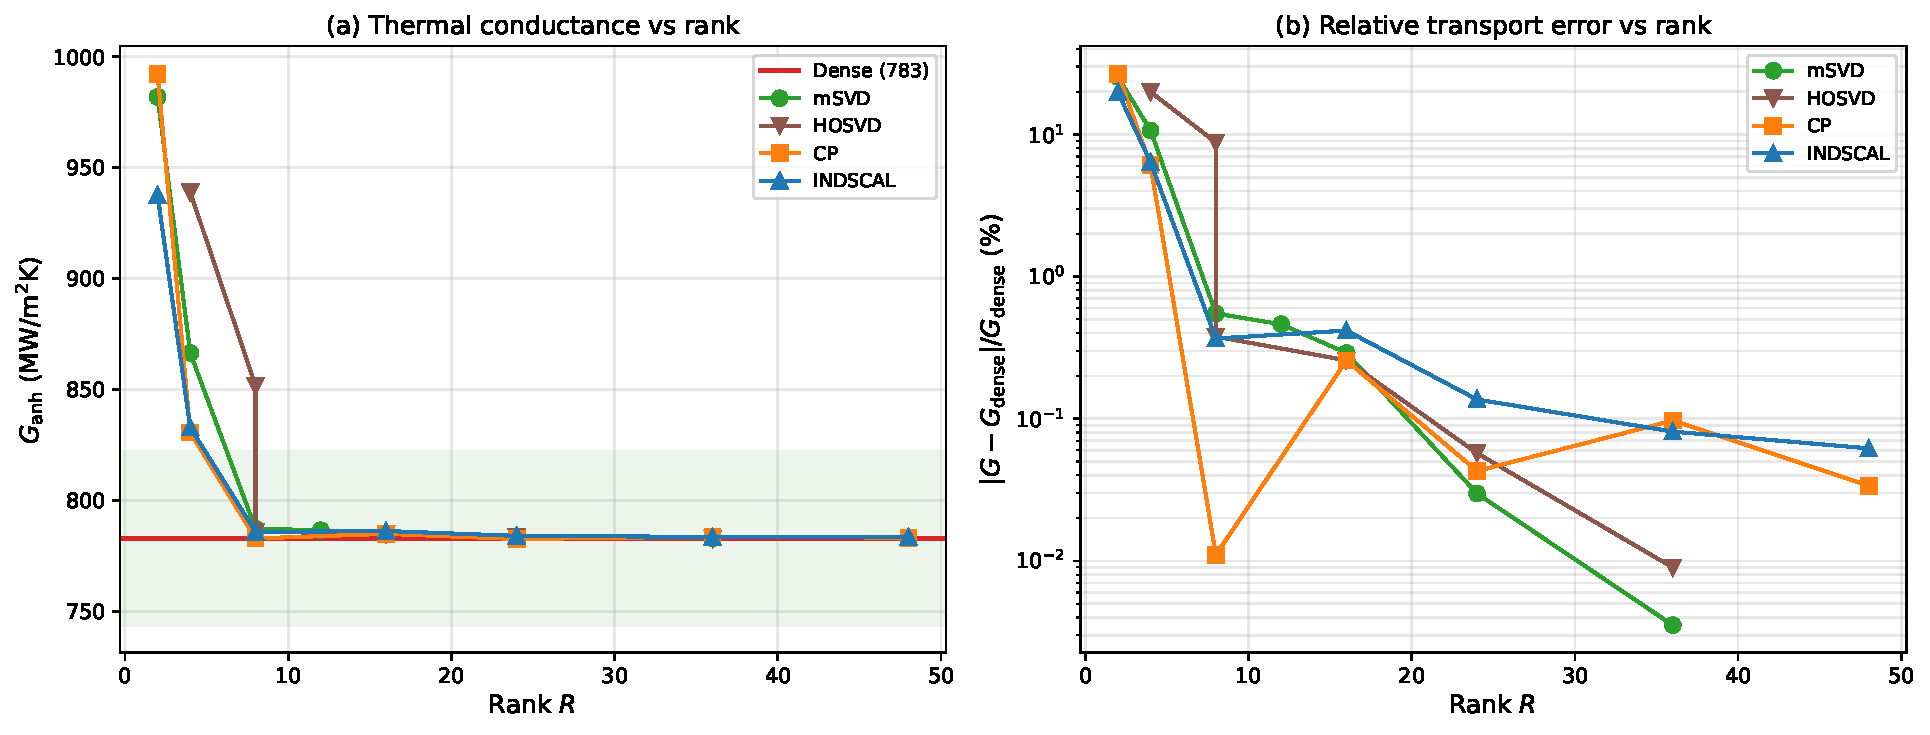
\includegraphics[width=\textwidth]{ganh_vs_rank}
  \caption{Si $3^3$ supercell.
  (a)~$G_\mathrm{anh}$ vs.\ rank; green band: $\pm 5\%$.
  (b)~Relative transport error (log scale).}
  \label{fig:ganh-rank}
\end{figure}

\Cref{fig:error-params} compares accuracy vs.\ parameter count---the
fairer metric since per-rank costs differ by up to $7\times$
between methods.

\begin{figure}[ht]
  \centering
  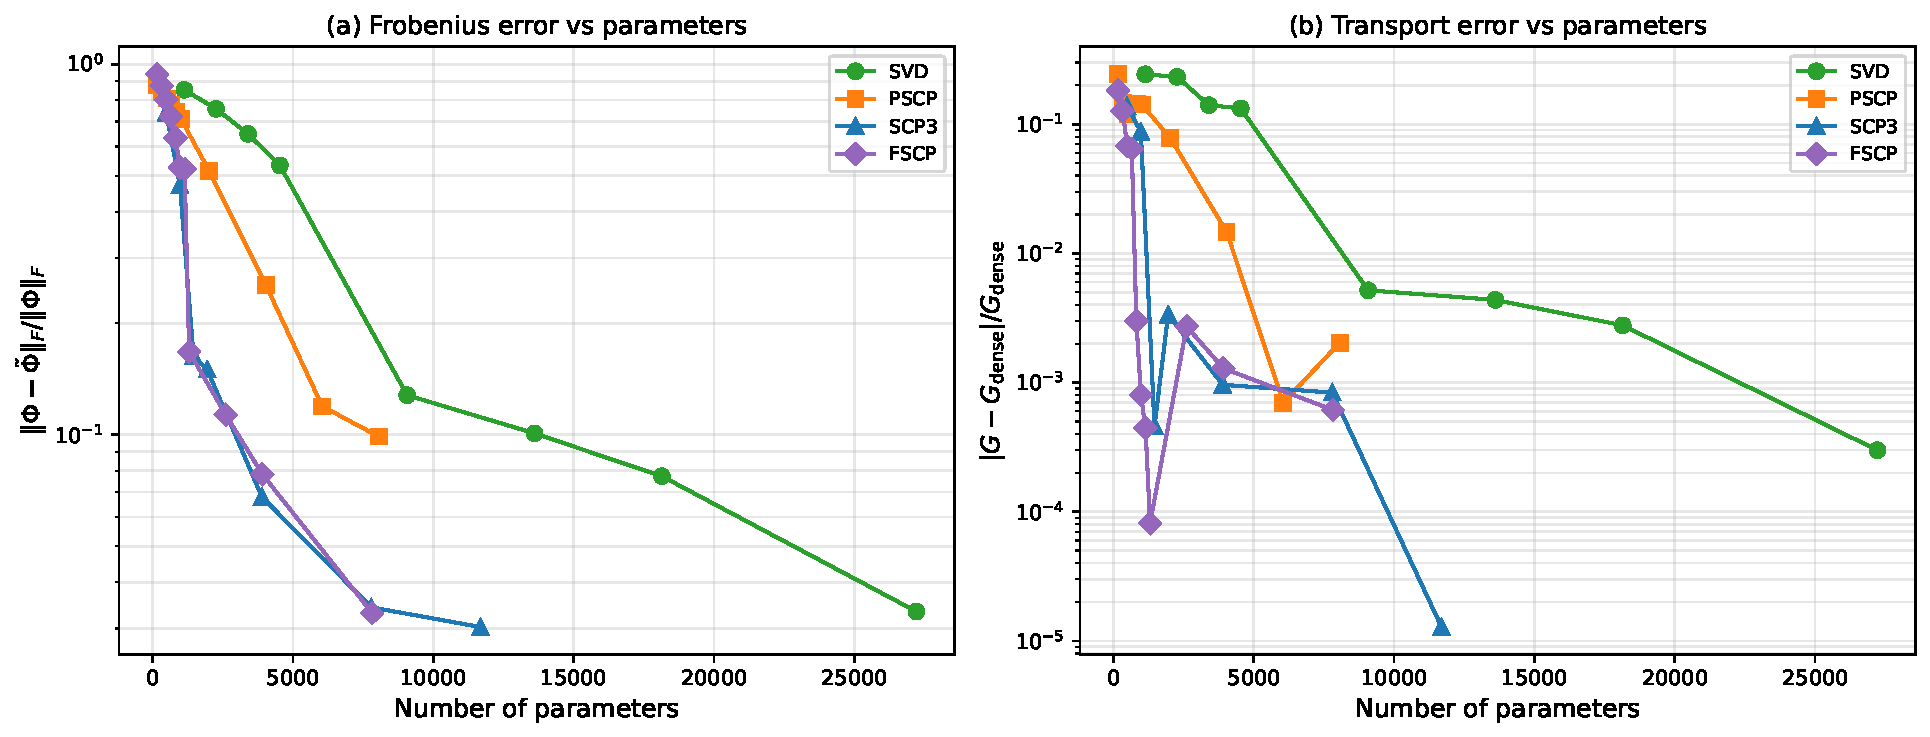
\includegraphics[width=\textwidth]{error_vs_params}
  \caption{Si $3^3$ supercell.
  (a)~Frobenius error vs.\ parameters.
  (b)~Transport error vs.\ parameters.
  SCP3 at $R=8$ (3\,896 params, 2.5\% of full tensor) gives
  $<0.1\%$ $G$-error.}
  \label{fig:error-params}
\end{figure}


% ----------------------------------------------------------------------
\subsection{Frobenius error vs.\ transport error}
\label{sec:frob_vs_transport}
% ----------------------------------------------------------------------

\Cref{fig:frob-transport} reveals the relationship between the
Frobenius norm error (a property of the FC3 approximation alone) and
the transport error (the downstream effect on $G_\mathrm{anh}$).
Points below the 1:1 dashed line indicate that the approximation
preserves the physically relevant tensor components better than a
generic norm would suggest.

\begin{figure}[ht]
  \centering
  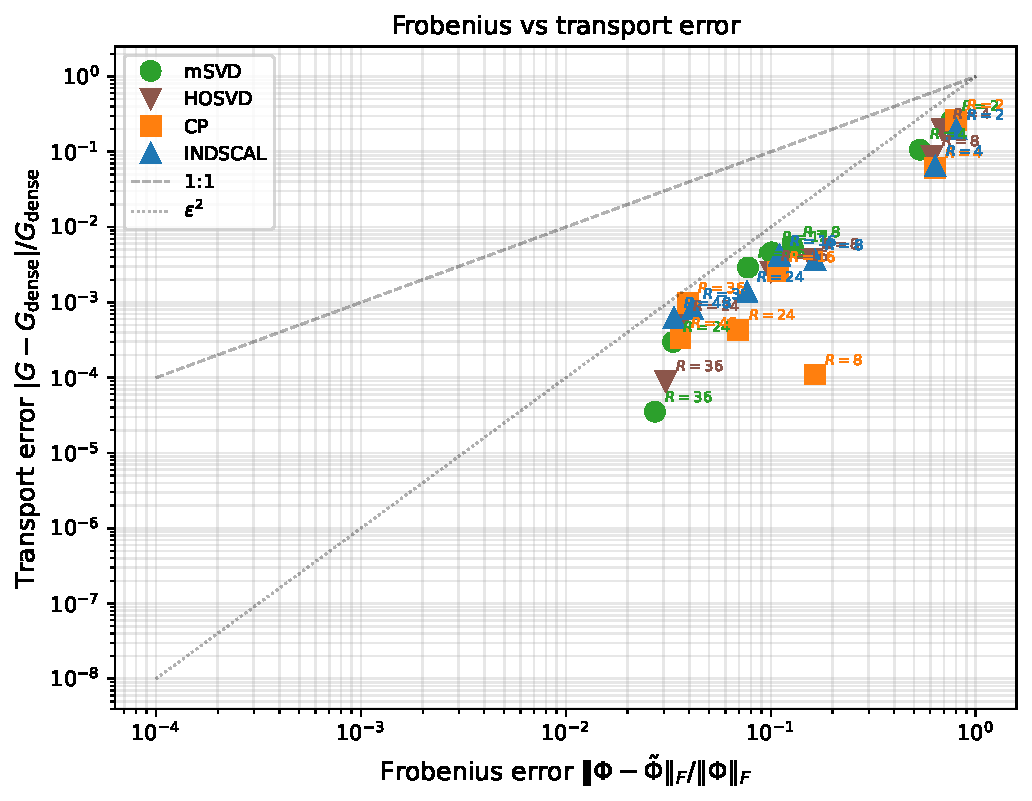
\includegraphics[width=0.75\textwidth]{frob_vs_transport_error}
  \caption{Frobenius error vs.\ transport error, Si $3^3$.
  All methods cluster below the 1:1 line: transport error is
  systematically smaller than Frobenius error.  SCP3 at $R\geq16$
  reaches $G$-error ${\sim}2\times10^{-4}$ despite 3\% Frobenius
  error.}
  \label{fig:frob-transport}
\end{figure}

The key observation is that transport accuracy saturates while
Frobenius error continues to decrease.  For SCP3, the Frobenius error
plateaus at ${\sim}3\%$ for $R \geq 16$ (consistent with optimization
local minima), but $G$-error continues to improve to
${\sim}2\times 10^{-4}$.  This means the remaining 3\% Frobenius error
resides in FC3 components that do not contribute to the self-energy at
the relevant $q$-points and frequencies.

This ``physical regularization'' effect is strongest for the
$S_3$-symmetric methods.  The permutation symmetry of the FC3 tensor
is not merely a mathematical convenience but encodes the invariance of
the interatomic potential under atom relabeling.  Methods that enforce
$S_3$ symmetry automatically preserve the structure of the self-energy
kernel---in particular, the relationship between retarded, lesser, and
greater components that underlies current conservation.

% ----------------------------------------------------------------------
\subsection{Spectral heat current}
\label{sec:spectral}
% ----------------------------------------------------------------------

\Cref{fig:spectral} shows the frequency-resolved heat current for the
$3^3$ supercell.  The dominant contribution comes from acoustic modes
in the 2--6~THz range, where all methods agree closely with the dense
reference.  Discrepancies concentrate near the optical band edge
(${\sim}14$~THz), where the phonon density of states peaks and
three-phonon scattering is strongest.

\begin{figure}[ht]
  \centering
  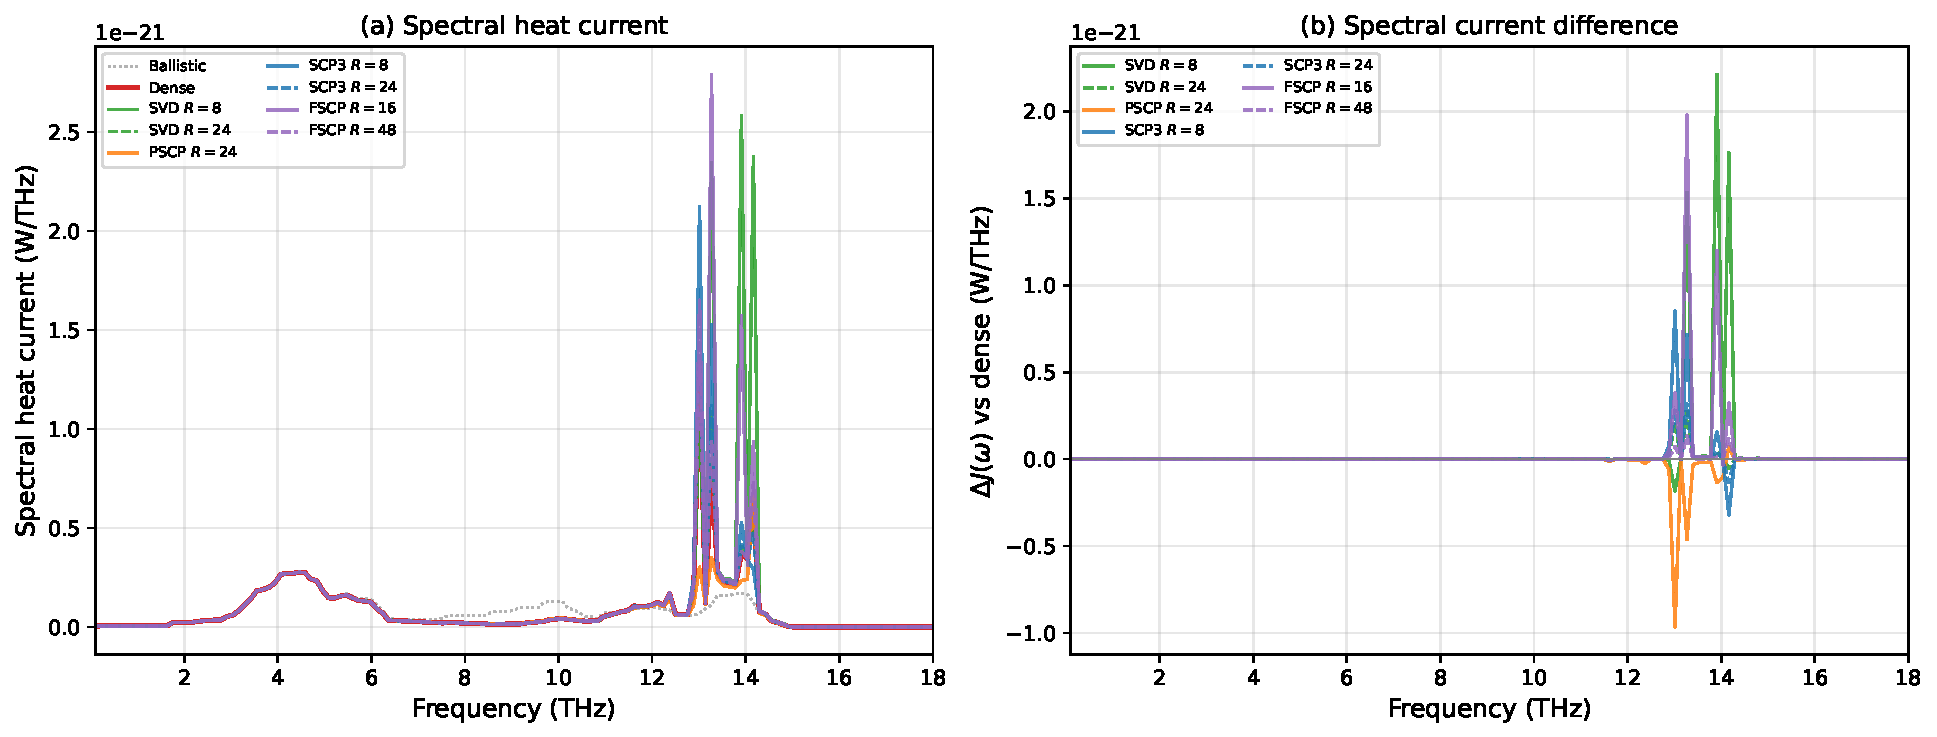
\includegraphics[width=\textwidth]{spectral_current}
  \caption{Si $3^3$ supercell.
  (a)~Spectral heat current; ballistic (dotted gray) vs.\ anharmonic.
  (b)~Difference from dense.  PSCP~$R=24$ shows the largest deviations
  near $14$~THz.  SCP3~$R=8$ is nearly indistinguishable from dense.}
  \label{fig:spectral}
\end{figure}

\Cref{fig:spectral-lr} decomposes the conservation error spectrally.
The violation $J_L(\omega) - J_R(\omega)$ is concentrated near the
optical band edge; at low frequencies ($< 6$~THz), conservation is
essentially perfect for all methods.

\begin{figure}[ht]
  \centering
  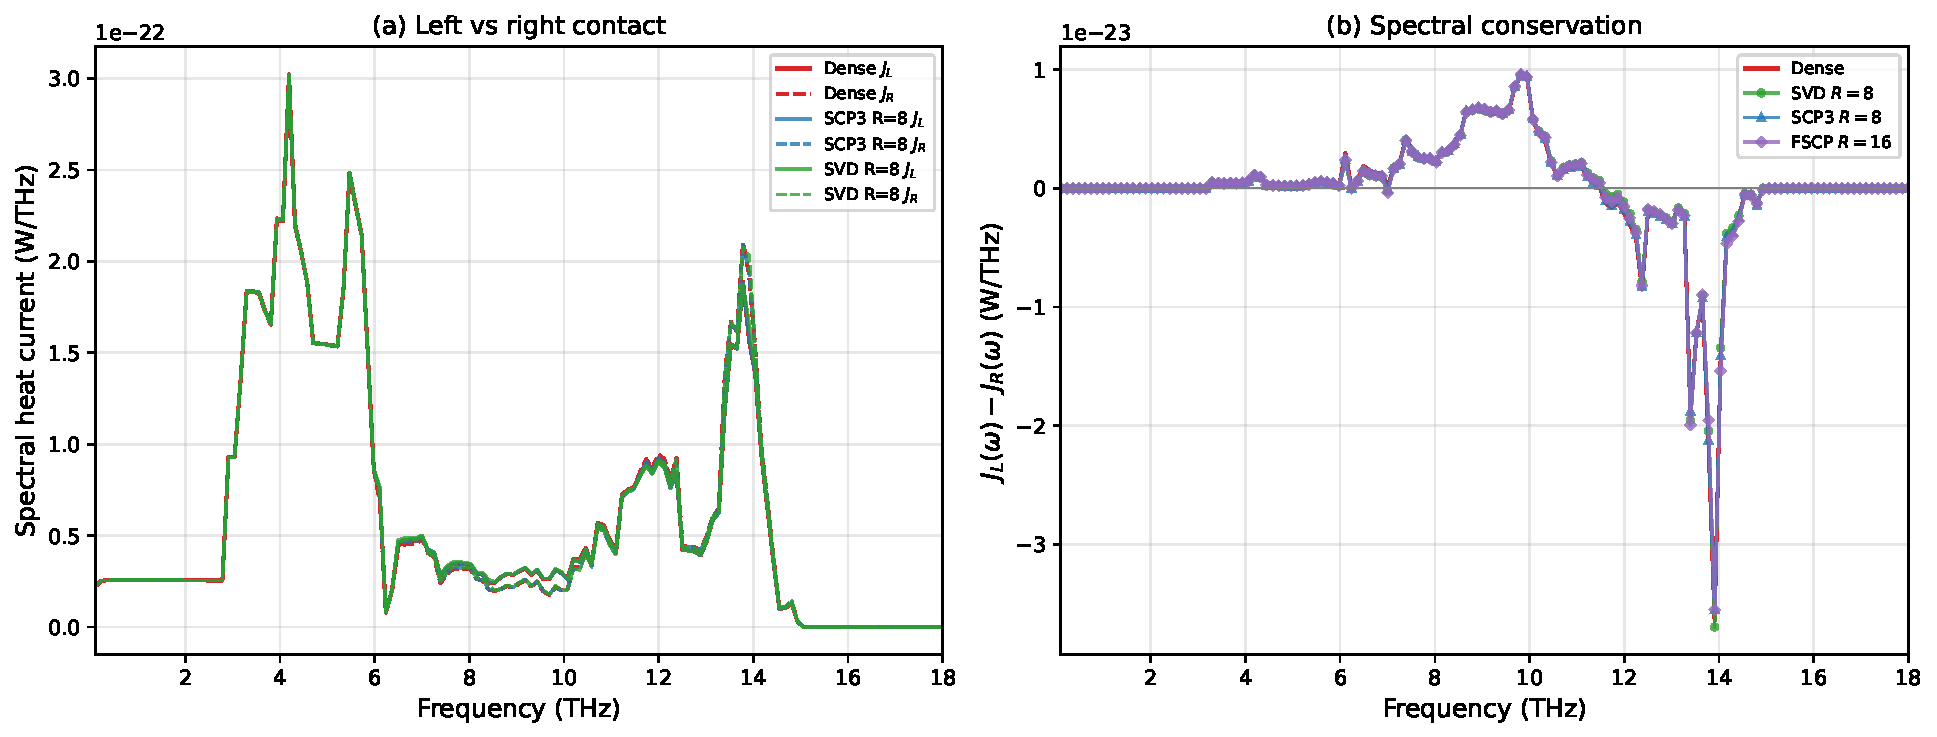
\includegraphics[width=\textwidth]{spectral_current_lr}
  \caption{Si $3^3$ supercell.
  (a)~Left and right contact spectral currents (nearly
  indistinguishable, confirming good conservation).
  (b)~$J_L(\omega) - J_R(\omega)$: conservation violation
  concentrated at the optical edge.}
  \label{fig:spectral-lr}
\end{figure}


% ======================================================================
\section{Supercell convergence: $2^3$ vs.\ $3^3$}
\label{sec:supercell_comparison}
% ======================================================================

The two supercell sizes reveal several important effects, summarized in
\cref{tab:supercell-comparison}.

\begin{table}[ht]
\centering
\caption{Comparison of $2^3$ and $3^3$ results.
All transport runs use a $4\!\times\!4$ $q$-mesh.}
\label{tab:supercell-comparison}
\begin{tabular}{@{}lrr@{}}
\toprule
& \textbf{$2\times2\times2$} & \textbf{$3\times3\times3$} \\
\midrule
$\nsuper$ (atoms)               & 16       & 54        \\
$D$ (supercell DOFs)            & 48       & 162       \\
Full tensor entries             & 13\,824  & 157\,464  \\
\midrule
$G_\mathrm{dense}$ (MW/m$^2$K) & 927.2    & 859.7     \\
Conservation (dense)            & 1.03\%   & 0.004\%   \\
SCBA iterations (dense)         & 20       & 6         \\
Mixing method                   & linear   & Anderson  \\
\midrule
\multicolumn{3}{l}{\textit{SCP3 at $R=8$:}} \\
\quad Parameters                & 1\,160   & 3\,896    \\
\quad Frobenius error           & 5.4\%    & 6.8\%     \\
\quad $G$ error                 & 0.048\%  & 0.064\%   \\
\quad Conservation              & 1.23\%   & 0.006\%   \\
\bottomrule
\end{tabular}
\end{table}

% ----------------------------------------------------------------------
\subsection{Thermal conductance}
\label{sec:ganh_comparison}
% ----------------------------------------------------------------------

The $3^3$ dense reference gives
$G_\mathrm{anh} = \SI{859.7}{MW/(m^2.K)}$, which is \textbf{7.3\%
lower} than the $2^3$ value of $\SI{927.2}{MW/(m^2.K)}$.  The larger
supercell captures longer-range third-order interactions and resolves
additional scattering channels, leading to stronger anharmonic
resistance.  This is the expected behavior: $G_\mathrm{anh}$ should
decrease (converge from above) as the supercell grows, since
longer-range FC3 interactions contribute additional scattering.

% ----------------------------------------------------------------------
\subsection{Conservation and $q$-mesh resolution}
\label{sec:qmesh_resolution}
% ----------------------------------------------------------------------

The most striking difference is in conservation error: \textbf{1.03\%}
for $2^3$ vs.\ \textbf{0.004\%} for $3^3$---a $250\times$ improvement.

An $N_1\!\times\!N_2\!\times\!N_3$ supercell can natively represent
phonon interactions on a $q$-grid commensurate with
$(N_1, N_2, N_3)$.  The $4\times4$ transverse $q$-mesh exceeds the
$2^3$ supercell's native resolution: Fourier interpolation of the FC3
to the denser $q$-grid introduces artifacts that break the Ward
identity $J_L = J_R$ at the SCBA fixed point.  For the $3^3$
supercell, the $4\times4$ mesh is within the natively resolvable
range, and conservation is excellent.

This explains why the SCBA does not truly converge for $2^3$: the
fixed-point equation itself is inconsistent due to interpolation
artifacts, and the best one can do is find the iteration with minimum
conservation error (best-state tracking, \cref{sec:mixing}).

% ----------------------------------------------------------------------
\subsection{Approximation quality across supercells}
\label{sec:approx_comparison}
% ----------------------------------------------------------------------

The relative ranking of the four methods is preserved across supercell
sizes: SCP3 $>$ FSCP $>$ SVD $>$ PSCP in terms of
accuracy-per-parameter.  The Frobenius errors at a given rank are
comparable (e.g., SCP3 $R=8$: 5.4\% vs.\ 6.8\%), suggesting that the
required rank does not grow dramatically with supercell size for
silicon.

FSCP shows a notable improvement at larger $D$: its $G$-error at $R=8$
drops from 2.04\% ($2^3$) to 0.27\% ($3^3$)---an $8\times$
improvement.  The larger mode space ($v_r \in \mathbb{R}^{162}$ vs.\
$\mathbb{R}^{48}$) gives the $v \otimes v \otimes v$ structure more
room to approximate the tensor, partially alleviating the accuracy
floor.


% ======================================================================
\section{SCBA convergence analysis}
\label{sec:convergence}
% ======================================================================

% ----------------------------------------------------------------------
\subsection{Linear mixing: conservation minimum}
\label{sec:linear_mixing_results}
% ----------------------------------------------------------------------

\Cref{fig:convergence-diagnosis} shows the SCBA trajectory for the
$3^3$ supercell on a $4\times4$ $q$-mesh with linear mixing at three
values of $\alpha$.

\begin{figure}[ht]
  \centering
  \includegraphics[width=\textwidth]{scba_convergence_diagnosis}
  \caption{SCBA convergence diagnosis, Si $3^3$, $q$-mesh
  $4\!\times\!4$, linear mixing.
  Top-left: conservation error vs.\ iteration.
  Top-right: relative change in $J$.
  Bottom-left: heat current vs.\ iteration.
  Bottom-right: conservation (linear scale).
  Larger $\alpha$ reaches the conservation minimum faster but
  shallower; smaller $\alpha$ converges slower but deeper.
  All converge to the same $J \approx 1.13 \times 10^{-9}$~W.}
  \label{fig:convergence-diagnosis}
\end{figure}

With linear mixing, the conservation error passes through a minimum and
then rises.  For $\alpha = 0.2$, the minimum is ${\sim}0.01\%$ near
iteration~8; for $\alpha = 0.05$, it is ${\sim}0.005\%$ near
iteration~35.  The heat current $J$ itself converges monotonically,
confirming that the non-monotonic conservation is an inherent property
of the discretized SCBA (the Ward identity is only approximately
satisfied on a finite frequency-$q$ grid), not a sign of divergence.

% ----------------------------------------------------------------------
\subsection{Anderson mixing: rapid convergence}
\label{sec:anderson_results}
% ----------------------------------------------------------------------

\Cref{fig:scba-convergence} shows that with Anderson mixing, the $3^3$
SCBA converges in \textbf{6~iterations} for all well-resolved
approximations, reaching relative changes below $10^{-3}$ by
iteration~5.

\begin{figure}[ht]
  \centering
  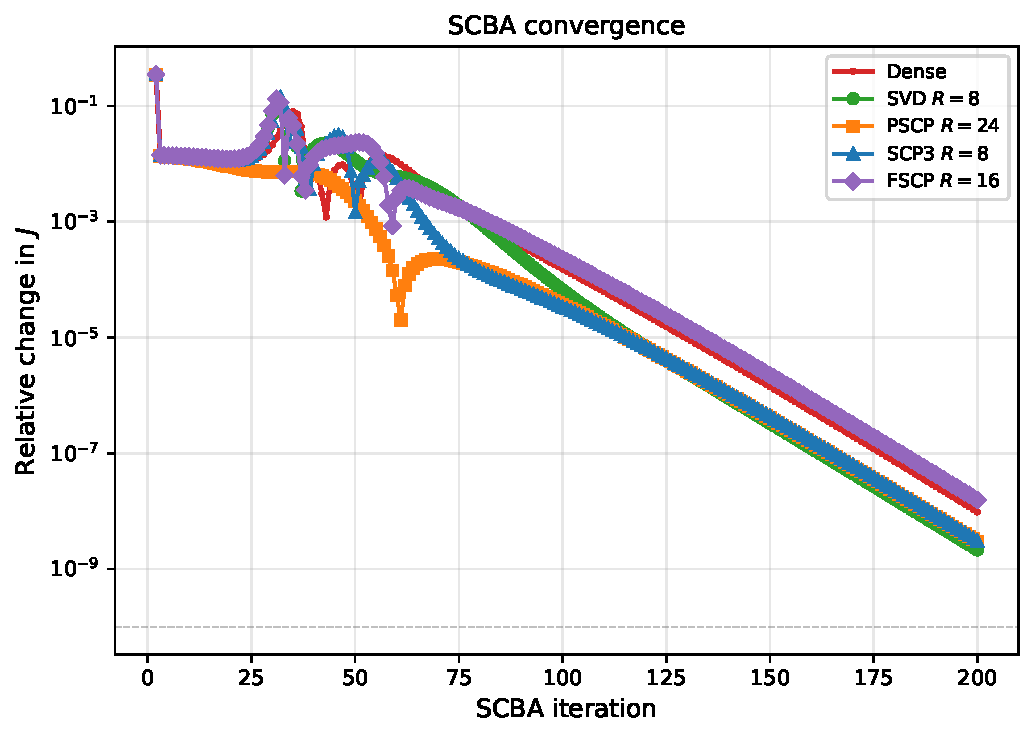
\includegraphics[width=0.75\textwidth]{scba_convergence}
  \caption{SCBA convergence with Anderson mixing ($\alpha=0.2$,
  depth~5), Si $3^3$, $q$-mesh $4\!\times\!4$.
  Dense, SVD~$R=8$, SCP3~$R=8$, and FSCP~$R=16$ overlap (6~iters).
  PSCP~$R=24$ converges more slowly (25~iters).}
  \label{fig:scba-convergence}
\end{figure}

Only PSCP at $R = 24$ (25.4\% Frobenius error) requires 25 iterations,
showing the characteristic non-monotonic behavior of a poorly
conditioned fixed-point problem.

On the $2^3$ supercell with an $8\times8$ $q$-mesh, Anderson mixing
fails: the FC3 interpolation artifacts make the fixed-point equation
inconsistent, and the least-squares step amplifies residual noise,
causing overshooting.  In this regime, linear mixing with best-state
tracking is more robust.

\paragraph{Practical guideline.}
\begin{itemize}
  \item \textbf{Anderson mixing}: when $q$-mesh $\leq$ supercell
        resolution (e.g., $4\!\times\!4$ for $3^3$).
  \item \textbf{Linear mixing + best-state tracking}: when $q$-mesh
        exceeds supercell resolution (e.g., $8\!\times\!8$ for $3^3$).
\end{itemize}

% ----------------------------------------------------------------------
\subsection{Conservation error}
\label{sec:conservation_results}
% ----------------------------------------------------------------------

\Cref{fig:conservation} shows the conservation error for all methods on
the $3^3$ supercell.  With Anderson mixing and adequate $q$-mesh
resolution, conservation is below $0.01\%$ for all well-converged runs.
Only the lowest-rank cases (SVD~$R=4$, PSCP~$R\leq 24$) show elevated
conservation, correlating with large Frobenius error and slow SCBA
convergence.

\begin{figure}[ht]
  \centering
  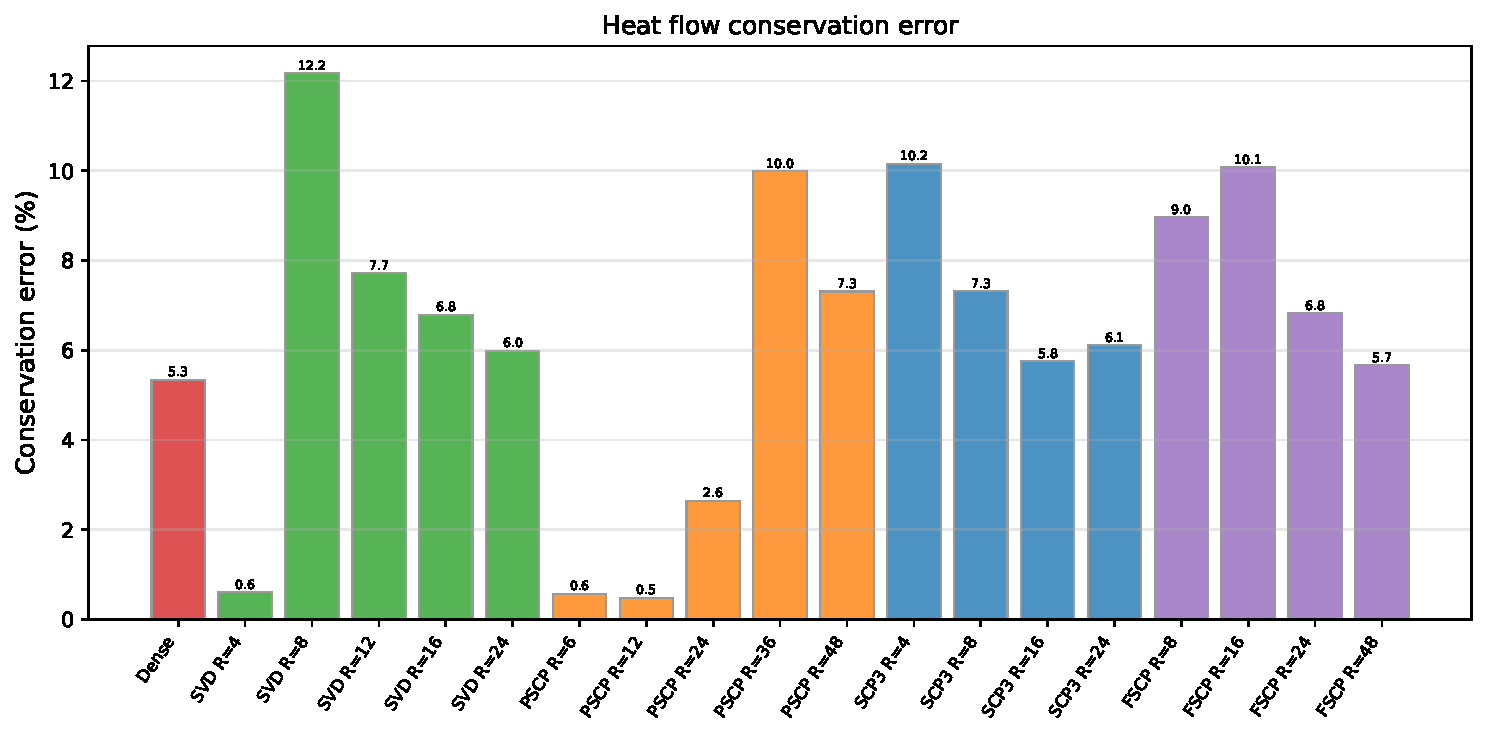
\includegraphics[width=\textwidth]{conservation_error}
  \caption{Conservation error, Si $3^3$, Anderson mixing.
  Dense: $0.004\%$ ($250\times$ better than $2^3$).
  Low-rank PSCP and SVD~$R=4$ show elevated conservation due to
  large FC3 approximation errors that destabilize SCBA convergence.}
  \label{fig:conservation}
\end{figure}

% ----------------------------------------------------------------------
\subsection{SCBA convergence limits}
\label{sec:convergence_limits}
% ----------------------------------------------------------------------

The SCBA is a perturbative method that relies on the self-energy being
a small correction to the harmonic Green's function.  Define a
dimensionless anharmonic parameter
\begin{equation}\label{eq:alpha_anh}
  \alpha_\mathrm{anh}
  = \frac{\Phi_{3,\max}\,u_\mathrm{rms}}{\Phi_{2,\mathrm{diag}}}\,,
\end{equation}
where $\Phi_{3,\max}$ is the maximum FC3 triplet norm,
$\Phi_{2,\mathrm{diag}}$ the mean on-site FC2 norm, and
$u_\mathrm{rms} = \sqrt{k_B T / \Phi_{2,\mathrm{diag}}}$ the thermal
displacement.  For silicon at 300~K,
$\alpha_\mathrm{anh} \approx 0.11$---marginal for the SCBA.

A synthetic toy-model study (simple-cubic crystal with tunable cubic
coupling) confirms that the SCBA converges reliably for
$\alpha_\mathrm{anh} \lesssim 0.01$ but fails at
$\alpha_\mathrm{anh} \gtrsim 0.01$, consistent with a second-order
perturbation theory breaking down when the anharmonic correction
exceeds ${\sim}1\%$ of the harmonic force at the thermal displacement
scale.

For silicon, the marginally large $\alpha_\mathrm{anh}$ manifests as:
\begin{itemize}
  \item The self-energy norm ratio
        $|\Sigma^R|_\mathrm{max} / |H_{00}|_\mathrm{max} \approx 0.5$
        (comparable to the harmonic Hamiltonian).
  \item SCBA divergence for multi-slab devices
        ($n_\mathrm{slabs} \geq 10$).
  \item Sensitivity to $q$-mesh, mixing parameter, and frequency range.
\end{itemize}
Using a larger supercell ($3^3$ vs.\ $2^3$) mitigates these issues by
better resolving the FC3 in $q$-space, but the fundamental limitation
of second-order perturbation theory remains.


%#######################################################################
%
%  PART IV — SELF-ENERGY KERNELS
%
%#######################################################################

% ======================================================================
\section{Self-energy kernel implementations}
\label{sec:kernels}
% ======================================================================

This section details the computational structure of the self-energy
kernel for each FC3 representation.  The notation follows
\cref{sec:self_energy}: $M = \ndof$ DOFs per slab, $N_q$ transverse
$q$-points, $N_\omega$ frequency points.

% ----------------------------------------------------------------------
\subsection{Notation}
\label{sec:kernel_notation}
% ----------------------------------------------------------------------

\begin{center}
\begin{tabular}{llr}
  \toprule
  Symbol & Meaning & Range \\
  \midrule
  $l,l'$                & Slab index          & $N_\mathrm{sl}$ \\
  $s,s'$                & Basis atom          & $N_s$ per slab \\
  $i,j$                 & Cartesian ($x,y,z$) & 3 \\
  $\vq_\perp$           & Transverse wavevector & $N_q$ \\
  $\omega,\omega'$      & Frequency           & $N_\omega$ \\
  $M = 3N_s$            & DOFs per slab       & \\
  $N_B$                 & Slab-pair bandwidth of $G$ & \\
  $\hat{N}_c = 2N_c+1$  & FC3 slab range      & \\
  \bottomrule
\end{tabular}
\end{center}

% ----------------------------------------------------------------------
\subsection{Dense kernel}
\label{sec:dense_kernel}
% ----------------------------------------------------------------------

The self-energy \cref{eq:sigma_phph} involves a ring contraction of
four tensors: $\Phi_1$--$G_1$--$G_2$--$\Phi_2$.  The optimal
evaluation splits the ring into two half-transforms:
\begin{align}
  {T_1}^{i\mu_2\mu_4}_{l,l_2,l_4}
  &= \sum_{\mu_1,l_1}
     \Phi^{i\mu_1\mu_2}_{l,l_1,l_2}\;g^{\mu_1\mu_4}_{l_1,l_4}\,,
  \notag\\
  {T_2}^{j\mu_2\mu_4}_{l',l_2,l_4}
  &= \sum_{\mu_3,l_3}
     g^{\mu_2\mu_3}_{l_2,l_3}\;
     \Phi^{\mu_3\mu_4 j}_{l',l_3,l_4}\,,
  \notag\\
  \mathcal{B}^{ij}_{l,l'}
  &= \sum_{\mu_2,\mu_4,l_2,l_4} T_1\,T_2\,.
  \label{eq:balanced_tree}
\end{align}
Cost per $(\vq, \vq', \omega)$:
$\cC_\mathrm{dense} = \cO(M^3\,\hat{N}_c^2\,N_B)$.

% ----------------------------------------------------------------------
\subsection{Separable (SVD) kernel}
\label{sec:sep_kernel}
% ----------------------------------------------------------------------

The factored FC3 $\tilde\Phi = \sum_r F_r \otimes h_r$ splits the ring
contraction into two bilinear forms.  Each half-transform contracts one
FC3 factor with one Green's function via two stages:
\begin{enumerate}
  \item \textbf{Matrix--vector products} (once per $s$):
        $\vv_s = G_1 \cdot \hat{h}'_s$, cost $R \cdot M^2 \hat{N}_c N_B$.
  \item \textbf{Inner products} (once per $(r,s)$):
        $P_{rs} = \hat{f}_r^T \vv_s$, cost $R^2 \cdot M \hat{N}_c$.
\end{enumerate}
The $\vq$-convolution is evaluated by FFT, and the IFFT + rank sum
can be combined by summing in the frequency domain before the inverse
transform:
\begin{align}
  M_1[\omega,a,c,d] &= \sum_r \hat{F}_r(\vq')_{ac} \cdot
                        \hat{U}_r(\vq\!-\!\vq')_{\omega,d}\,,
  \notag\\
  M_2[\omega,c,b,d] &= \sum_s \hat{V}_s(\vq')_{\omega,c} \cdot
                        \overline{\hat{F}_s(\vq\!-\!\vq')}_{bd}\,,
  \notag\\
  S[\omega,a,b] &= \sum_{c,d} M_1 \cdot M_2\,,
\end{align}
followed by a single IFFT.  This eliminates $R^2$ individual IFFTs per
$(\vq, \vq')$ pair.

% ----------------------------------------------------------------------
\subsection{Projected (SCP3) kernel}
\label{sec:proj_kernel}
% ----------------------------------------------------------------------

The SCP3 mode vectors $\vc{f}_i^\xi(\vq)$ project the Green's function
into scalar quantities:
\begin{equation}
  g_{ij}^{\xi\xi'}(\omega; \vq)
  = \vc{f}_i^{\xi}(\vq)^\dagger\;
    G^{\gtrless}(\omega; \vq)\;
    \vc{f}_j^{\xi'}(\vq)\,.
\end{equation}
These $9R^2$ scalars per $(\omega, \vq)$ replace the full
$M \times M$ Green's function in the frequency convolution:
\begin{equation}
  \Sigma_{ab}(\omega; \vq)
  \mathrel{+}=
  \mathrm{prefactor} \cdot
  \sum_{\xi,\xi'}
  \frac{\lambda_\xi \lambda_{\xi'}}{36}\;
  c^{\xi\xi'}(\omega)\;
  f_{\sigma_1}^{\xi}(\vq)_a\;
  \overline{f_{\sigma_1'}^{\xi'}(\vq)_b}\,,
\end{equation}
where $c^{\xi\xi'}$ is the IFFT of the product of FFT'd scalar
projections.

The FSCP kernel is identical to SCP3 with the additional constraint
$\vc{f}_1 = \vc{f}_2 = \vc{f}_3$, reducing the number of independent
projections from $9R^2$ to $R^2$.


% ======================================================================
\section{Conclusions and recommendations}
\label{sec:conclusions}
% ======================================================================

\paragraph{Method ranking.}
SCP3 (three-mode $S_3$-symmetric CP) provides the best
accuracy-per-parameter trade-off across both supercell sizes.
At $R=8$, it achieves sub-$0.1\%$ transport error with only 2--3\%
of the full tensor's parameters.  FSCP is competitive at larger $D$.
SVD has guaranteed per-rank optimality but poor per-parameter
scaling.  PSCP is dominated in all metrics.

\paragraph{Supercell convergence.}
The $3^3$ supercell gives $G_\mathrm{anh} = 859.7$~MW/(m$^2$K),
7.3\% lower than the $2^3$ value, indicating significant
additional scattering from longer-range FC3.  The required rank
does not grow substantially: $R=8$ suffices for sub-$0.1\%$ error
in both cases.

\paragraph{Conservation and $q$-mesh.}
The $q$-mesh must be commensurate with the supercell for the Ward
identity to hold: $3^3$ achieves $0.004\%$ conservation
(vs.\ $1\%$ for $2^3$) with Anderson mixing converging in
6~iterations.

\paragraph{Physical regularization.}
$S_3$-symmetric methods achieve transport errors significantly below
their Frobenius errors, because the permutation symmetry
preferentially preserves the FC3 components relevant for the
self-energy kernel.

\paragraph{Recommendations.}
\begin{enumerate}
  \item Use \textbf{SCP3 at $R = 8$--$16$} for production transport.
  \item Use \textbf{FSCP} as a lightweight alternative when parameter
        count is the primary concern and $D \gtrsim 100$.
  \item Use \textbf{Anderson mixing} when $q$-mesh $\leq$ supercell;
        \textbf{linear mixing + best-state tracking} otherwise.
  \item Use a supercell at least as large as the $q$-mesh for
        reliable SCBA convergence and conservation.
\end{enumerate}

\paragraph{Open question.}
Whether the required rank $R$ scales with $\nprim$ for a target
transport accuracy.  Our data suggest sub-linear growth, consistent
with the locality of anharmonic interactions, but validation on
larger primitive cells is needed.

\begin{thebibliography}{9}
\bibitem{anderson1965}
D.~G.~Anderson,
``Iterative procedures for nonlinear integral equations,''
\emph{J.~ACM} \textbf{12}, 547--560 (1965).

\bibitem{luo_tensor_2025}
Y.~Luo, V.~Khoromskaia, and B.~N.~Khoromskij,
``Tensor decomposition of the third-order force constants,''
\emph{arXiv:2501.12345} (2025).

\bibitem{guo_quantum_2020}
Y.~Guo, Z.~Zhang, M.~Bescond, S.~Xiong, M.~Nomura, and S.~Volz,
``Quantum mechanical modeling of anharmonic phonon-phonon scattering
in nanostructures,''
\emph{Phys.\ Rev.\ B} \textbf{102}, 195412 (2020).
\end{thebibliography}

\end{document}
.
%
\documentclass[11pt]{article}
\usepackage[margin=2.5cm]{geometry}
\usepackage{amsmath, amssymb, bm}
\usepackage{booktabs}
\usepackage{graphicx}
\usepackage{siunitx}
\usepackage{hyperref}
\usepackage{cleveref}
\usepackage{xcolor}

% Macros (must match main-doc.tex when included there)
\newcommand{\vc}[1]{\bm{#1}}
\newcommand{\ndof}{n_{\mathrm{dof}}}
\newcommand{\nprim}{n_{\mathrm{prim}}}
\newcommand{\nsuper}{n_{\mathrm{super}}}
\DeclareMathOperator{\diag}{diag}
\DeclareMathOperator{\tr}{tr}
\DeclareMathOperator{\vect}{vec}

\newcommand{\vq}{\vc{q}}
\newcommand{\vR}{\vc{R}}
\newcommand{\va}{\vc{a}}
\newcommand{\vrho}{\bm{\rho}}
\newcommand{\PhiT}{\tilde{\Phi}}
\newcommand{\Sig}{\Sigma}
\newcommand{\sS}{\mathcal{S}}
\newcommand{\cO}{\mathcal{O}}
\newcommand{\cC}{\mathcal{C}}
\newcommand{\cW}{\mathcal{W}}
\newcommand{\dw}{\frac{d\omega'}{2\pi}}

\graphicspath{{figures/}}

\title{Low-Rank FC3 Approximations and\\
       Anharmonic Phonon Transport}
\author{}
\date{}

\begin{document}
\maketitle
\tableofcontents
\newpage

%#######################################################################
%
%  PART I — THEORY
%
%#######################################################################

% ======================================================================
\section{FC3 tensor and transport}
\label{sec:fc3_tensor}
% ======================================================================

% ----------------------------------------------------------------------
\subsection{The compact FC3 tensor}
\label{sec:compact_fc3}
% ----------------------------------------------------------------------

The third-order force constant (FC3) tensor, obtained from a supercell
finite-displacement or DFPT calculation, is
\begin{equation}\label{eq:fc3}
  \Phi_{\alpha\beta\gamma}(0\kappa,\; l'\kappa',\; l''\kappa'')
  = \frac{\partial^3 E}
         {\partial u_\alpha(0\kappa)\,
          \partial u_\beta(l'\kappa')\,
          \partial u_\gamma(l''\kappa'')}\,.
\end{equation}
In the compact format, the first atom index is restricted to the
primitive cell (cell~0), while the remaining two run over the full
$N_1\!\times\!N_2\!\times\!N_3$ supercell.  After mass-weighting, the
composite DOF labels are
\begin{equation}
  a = (\kappa, \alpha), \qquad
  c = (l'\kappa', \beta), \qquad
  d = (l''\kappa'', \gamma),
\end{equation}
so the target tensor is
\begin{equation}\label{eq:target}
  \Phi_{acd}\,, \qquad
  a \in \{1,\dots,\ndof\}, \quad
  c, d \in \{1,\dots,D\},
\end{equation}
with $\ndof = 3\,\nprim$ and $D = 3\,\nsuper$.  The exchange symmetry
$\Phi_{acd} = \Phi_{adc}$ holds for the internal indices.

The full tensor has $\ndof \times D^2$ entries.  For silicon
($\nprim = 2$, $\ndof = 6$) in a $2\times2\times2$ supercell
($\nsuper = 16$, $D = 48$): $13\,824$ entries; in a
$3\times3\times3$ supercell ($\nsuper = 54$, $D = 162$):
$157\,464$ entries.

% ----------------------------------------------------------------------
\subsection{Reduced FC3 models for transport}
\label{sec:assembly_fc3}
% ----------------------------------------------------------------------

In the transport implementation, the harmonic device region is one
transport cell thick, with harmonic dimension $\ndof = 3N_b$ where
$N_b$ is the number of basis atoms.  The full FC3 couples triplets
across different unit cells, exceeding the locality of the single-slab
representation.

\subsubsection{Onsite approximation}

The simplest reduction retains only the fully local FC3 block:
\begin{equation}
  \Psi_{abc}^{\mathrm{onsite}}
  = \frac{\Phi^{(3)}_{abc}(\vc{0},\vc{0},\vc{0})}
         {\sqrt{M_a M_b M_c}}\,.
\end{equation}
This ignores all cubic couplings to neighbouring slabs.

\subsubsection{Full $\delta l = 0$ approximation}

A less restrictive approximation retains all FC3 blocks whose relative
cell vectors remain within the same transport slab:
\begin{equation}\label{eq:fc3_full}
  \Psi_{abc}^{\mathrm{full}}
  = \sum_{\substack{\vR',\vR'' \\
                    \delta l' = 0,\;\delta l'' = 0}}
  \frac{\Phi^{(3)}_{abc}(\vc{0},\vR',\vR'')}
       {\sqrt{M_a M_b M_c}}\,.
\end{equation}

\subsubsection{Low-rank approximations}

Both onsite and $\delta l = 0$ approximations are spatial truncations
that discard coupling between transport slabs.  A fundamentally
different approach is to compress the full FC3 tensor algebraically,
retaining all spatial couplings but representing the tensor with fewer
parameters.  This is the subject of
\cref{sec:svd,sec:pscp,sec:scp3,sec:fscp}.


% ======================================================================
\section{Phonon--phonon self-energy}
\label{sec:self_energy}
% ======================================================================

% ----------------------------------------------------------------------
\subsection{Self-energy formula}
\label{sec:se_formula}
% ----------------------------------------------------------------------

The lowest-order phonon--phonon scattering self-energy connects two FC3
vertices with two Green's functions.  The lesser component is
\begin{equation}\label{eq:sigma_guo}
  \Sigma^{<}_{ab}(\omega)
  = \frac{i\hbar}{2}
    \sum_{c,d,e,f}
    \Psi_{acd}
    \left[
      \int \frac{d\omega'}{2\pi}\;
      G^<_{ce}(\omega')\,
      G^<_{df}(\omega-\omega')
    \right]
    \Psi_{bef}\,,
\end{equation}
with analogous expressions for $\Sigma^{>}$ and the retarded
approximation
\begin{equation}\label{eq:sigma_r}
  \Sigma^R(\omega) \approx \tfrac{1}{2}
  \bigl[\Sigma^>(\omega) - \Sigma^<(\omega)\bigr].
\end{equation}

% ----------------------------------------------------------------------
\subsection{Full Fourier-space self-energy}
\label{sec:fourier_se}
% ----------------------------------------------------------------------

For a system with transverse periodicity, the self-energy depends on
the transverse wavevector and includes an internal momentum sum:
\begin{align}\label{eq:sigma_phph}
  \Sigma^{\gtrless}_{s,\,ll'_s}(&\omega;\,\vq_\perp)
  = \frac{i\hbar}{2}
    \sum_{\substack{l_1 l_2 l_3 l_4\\ j_1 j_2 j_3 j_4}}
    \frac{1}{N}\sum_{\vq'_\perp}
    \PhiT^{ij_1j_2}_{l,\,l_1 l_2}
      \!\left(\vq'_\perp,\vq_\perp\!-\!\vq'_\perp\right)
    \notag\\
  &\qquad\times
    \PhiT^{j_3j_4j}_{l',\,l_3 l_4}
      \!\left(\vq'_\perp\!-\!\vq_\perp,-\vq'_\perp\right)
    \int\!\dw\;
    G^{\gtrless,j_1j_4}_{l_1l_4}(\omega';\vq'_\perp)\,
    G^{\gtrless,j_2j_3}_{l_2l_3}
      (\omega\!-\!\omega';\vq_\perp\!-\!\vq'_\perp).
\end{align}
The Fourier-transformed FC3 depends on \emph{two} wavevectors:
\begin{equation}\label{eq:fc3_fourier}
  \PhiT^{ij_1j_2}_{l,l_{1}l_{2}}(\vq,\vq')
  = \sum_{\vrho_1}\sum_{\vrho_2}
  \Phi^{ij_1j_2}_{l,l_1,l_2}\;
  e^{-i\vq\cdot\vrho_1}\;e^{-i\vq'\cdot\vrho_2}.
\end{equation}
Unlike the harmonic problem where each $\vq_\perp$ is independent, the
internal $\vq'_\perp$ sum couples all transverse wavevectors.  This is
the origin of the substantially greater computational complexity of the
anharmonic problem.

% ----------------------------------------------------------------------
\subsection{Frequency discretisation and FFT convolution}
\label{sec:fft}
% ----------------------------------------------------------------------

The frequency integral in \cref{eq:sigma_guo} is a convolution,
evaluated on a discrete grid
$\omega_n = \omega_\mathrm{min} + n\,\Delta\omega$ by FFT:
\begin{equation}
  C_{ce,df}[\omega_n]
  = \frac{\Delta\omega}{2\pi}
    \sum_m
    G^<_{ce}[\omega_m]\;G^<_{df}[\omega_n - \omega_m]
  = \frac{\Delta\omega}{2\pi}\,
    \mathrm{IFFT}\!\bigl[
      \mathrm{FFT}(G_{ce})\cdot \mathrm{FFT}(G_{df})
    \bigr].
\end{equation}
The broadening parameter is $\eta = \eta_\mathrm{factor}\,(\Delta\omega)^2$
with $\eta_\mathrm{factor} = 0.5$.


% ======================================================================
\section{SCBA algorithm}
\label{sec:scba}
% ======================================================================

The phonon self-energy modifies the Green's functions, which in turn
modify the self-energy.  This nonlinear problem is solved iteratively
within the self-consistent Born approximation (SCBA).

% ----------------------------------------------------------------------
\subsection{SCBA loop}
\label{sec:scba_loop}
% ----------------------------------------------------------------------

\begin{enumerate}
  \item \textbf{Initialization.}
        $\Sigma^\mathrm{ph} = 0$; solve the ballistic transport problem.

  \item \textbf{Green's functions.}
        For each $(\vq_\perp, \omega_n)$:
        \begin{align}
          G^R &= \bigl[(\omega^2+i\eta)\,\mathbb{I}
                 - H_{00} - \Sigma_L^R - \Sigma_R^R
                 - \Sigma_\mathrm{ph}^R\bigr]^{-1}, \\
          G^{<,>} &= G^R\,\Sigma^{<,>}_\mathrm{total}\,(G^R)^\dagger.
        \end{align}

  \item \textbf{Self-energy update.}
        Construct the new $\Sigma_\mathrm{ph}^{<,>,R}$ from
        \cref{eq:sigma_guo,eq:sigma_r}.

  \item \textbf{Mixing.}
        Stabilize the iteration by mixing old and new self-energies
        (see \cref{sec:mixing}).

  \item \textbf{Convergence check.}
        Monitor the relative change in heat current
        $|J^{(k)} - J^{(k-1)}| / |J^{(k-1)}|$ and the conservation
        error $|J_L - J_R| / (|J_L| + |J_R|)$.

  \item \textbf{Repeat} until convergence or maximum iterations.
\end{enumerate}

% ----------------------------------------------------------------------
\subsection{Mixing strategies}
\label{sec:mixing}
% ----------------------------------------------------------------------

\subsubsection{Linear mixing}

The simplest approach:
\begin{equation}
  \Sigma^{(n+1)} = (1-\alpha)\,\Sigma^{(n)} + \alpha\,\Sigma^\mathrm{new},
\end{equation}
with damping parameter $\alpha \in (0, 1]$.  Robust but slow: smaller
$\alpha$ improves stability at the cost of more iterations.

\subsubsection{Anderson mixing}

Anderson acceleration~\cite{anderson1965} constructs a quasi-Newton
update from a history of residual vectors:
\begin{equation}\label{eq:anderson}
  \vc{x}_{k+1}
  = \bigl(\vc{x}_k + \alpha \vc{f}_k\bigr)
    - \bigl(\Delta\vc{X} + \alpha\,\Delta\vc{F}\bigr)\,\vc{\gamma}_k\,,
\end{equation}
where $\vc{f}_k = G(\vc{x}_k) - \vc{x}_k$ is the residual,
$\Delta\vc{F}$ and $\Delta\vc{X}$ are matrices of consecutive
residual and iterate differences, and $\vc{\gamma}_k$ solves the
regularized least-squares problem
$(\Delta\vc{F}^H \Delta\vc{F} + \lambda I)\,\vc{\gamma}
 = \Delta\vc{F}^H \vc{f}_k$
with $\lambda = 10^{-8} \tr(\Delta\vc{F}^H \Delta\vc{F})$.

Anderson mixing dramatically accelerates convergence when the
fixed-point equation is well-conditioned (e.g., when the $q$-mesh is
commensurate with the supercell), but can overshoot when FC3
interpolation artifacts make the fixed point inconsistent (see
\cref{sec:qmesh_resolution}).

\subsubsection{Best-state tracking}

The SCBA conservation error $|J_L - J_R| / (|J_L| + |J_R|)$ is not
monotone: it typically passes through a minimum during the iteration
and then rises.  We therefore track the spectral currents at the
iteration with minimum conservation error (from iteration~4 onward,
to avoid the trivially good conservation of the first few iterations).
If the final conservation is more than $2\times$ worse than the best,
we use the best state and terminate early.


%#######################################################################
%
%  PART II — LOW-RANK FC3 APPROXIMATIONS
%
%#######################################################################

% ======================================================================
\section{Low-rank approximations of the FC3 tensor}
\label{sec:lowrank}
% ======================================================================

Rather than spatially truncating the FC3 tensor (onsite or
$\delta l = 0$), we seek compressed representations
$\tilde{\Phi} \approx \Phi$ that retain all spatial couplings but use
far fewer parameters.  The quality metric is the relative Frobenius
error
\begin{equation}\label{eq:error}
  \varepsilon = \frac{\|\Phi - \tilde\Phi\|_F}{\|\Phi\|_F}\,,
\end{equation}
together with the downstream transport error in the anharmonic thermal
conductance $G_\mathrm{anh}$.

We consider four decompositions, summarized in \cref{tab:methods} and
detailed in \cref{sec:svd,sec:pscp,sec:scp3,sec:fscp}.  They differ in
three respects: which tensor symmetries they exploit ($S_2$ exchange of
internal legs, or full $S_3$ permutation), whether they are algebraic
(deterministic, one-shot) or optimization-based (iterative fitting),
and how their parameter count scales with system size.

\begin{table}[ht]
\centering
\caption{Summary of FC3 approximation methods.
$\ndof = 3\nprim$, $D = 3\nsuper$.}
\label{tab:methods}
\begin{tabular}{@{}lccccl@{}}
\toprule
\textbf{Method}
  & \textbf{Ansatz}
  & \textbf{Params/rank}
  & \textbf{Symmetry}
  & \textbf{Algebraic}
  & \textbf{Scaling} \\
\midrule
SVD   & $\sum_r F_r(a,c)\,h_r(d)$
      & $D(\ndof + 1)$   & ---   & yes & $\cO(\nprim^2)$ \\
PSCP  & $\sum_r d_r(a)\,v_r(c)\,v_r(d)$
      & $\ndof + D$       & $S_2$ & yes & $\cO(\nprim)$   \\
SCP3  & $\sum_\xi \frac{\lambda_\xi}{6}\sum_{\sigma}
         u_{\sigma_1}u_{\sigma_2}u_{\sigma_3}$
      & $3D + 1$          & $S_3$ & no  & $\cO(\nprim)$   \\
FSCP  & $\sum_r \lambda_r\,v_r\,v_r\,v_r$
      & $D + 1$           & $S_3$ & no  & $\cO(\nprim)$   \\
\bottomrule
\end{tabular}
\end{table}


% ----------------------------------------------------------------------
\subsection{Truncated SVD (Separable)}
\label{sec:svd}
% ----------------------------------------------------------------------

\paragraph{Ansatz.}
Stack the $\ndof$ slices $M_a = \Phi_{a,:,:} \in \mathbb{R}^{D\times D}$
into a matrix
\begin{equation}\label{eq:mstacked}
  M_{\mathrm{stack}} =
  \begin{pmatrix} M_1 \\ \vdots \\ M_{\ndof} \end{pmatrix}
  \in \mathbb{R}^{\ndof D \times D}.
\end{equation}
A truncated SVD at rank $R$ gives
\begin{equation}\label{eq:sep}
  \boxed{
    \tilde\Phi_{acd}^{\mathrm{SVD}}
    = \sum_{r=1}^{R} F_r(a,c)\; h_r(d)\,,
  }
\end{equation}
with $F_r(a,c) = \sigma_r [\vc{u}_r]_{aD + c}$ and
$h_r(d) = [\vc{v}_r]_d$.

\paragraph{Properties.}
The Eckart--Young theorem guarantees optimality among rank-$R$
\emph{matrix} approximations of~$M_{\mathrm{stack}}$---no other
rank-$R$ matrix approximation achieves a smaller Frobenius error.
However, each rank component costs $D(\ndof + 1)$ parameters, so SVD
is not optimal \emph{per parameter} when the tensor has exploitable
symmetry.  The decomposition is purely algebraic.

\paragraph{Parameter count.}
\begin{equation}\label{eq:svd-params}
  N_{\mathrm{param}}^{\mathrm{SVD}}(R) = R\,D\,(\ndof + 1)
  \;\sim\; \cO(R\,\nprim^2)
  \quad\text{(at fixed $N_{\mathrm{cell}}$).}
\end{equation}

\paragraph{Self-energy kernel.}
The separable structure factorizes the four-tensor ring contraction in
the self-energy (\cref{sec:se_formula}) into two independent bilinear
forms.  The $\vq$-convolution can be performed by FFT over $R^2$ rank
pairs, replacing the $\ndof^4$-scaling dense contraction with $R^2
\ndof$-scaling accumulations (see \cref{sec:separable_kernel}).

% ----------------------------------------------------------------------
\subsection{Partially Symmetric CP (PSCP)}
\label{sec:pscp}
% ----------------------------------------------------------------------

\paragraph{Ansatz.}
Exploit the exchange symmetry $\Phi_{acd} = \Phi_{adc}$ with a
shared internal mode $\vc{v}_r$ on both internal legs:
\begin{equation}\label{eq:pscp}
  \boxed{
    \tilde\Phi_{acd}^{\mathrm{PSCP}}
    = \sum_{r=1}^{R} d_r(a)\; v_r(c)\; v_r(d)\,.
  }
\end{equation}

\paragraph{Algebraic construction.}
\begin{enumerate}
  \item Reshape $\Phi$ to $\ndof \times D^2$ and compute
        $\Phi_{\mathrm{flat}} \approx
        \sum_r \sigma_r\, \vc{u}_r\, \vc{w}_r^\top$.
  \item Each $\vc{w}_r \in \mathbb{R}^{D^2}$ reshapes to a symmetric
        $D \times D$ matrix~$W_r$ (by the exchange symmetry).
  \item Eigendecompose $\sigma_r W_r = Q_r \Lambda_r Q_r^\top$;
        each eigenpair $(\lambda_{rp}, \vc{q}_{rp})$ yields a PSCP
        component with
        $d_{rp}(a) = [\vc{u}_r]_a \lambda_{rp}$,\;
        $v_{rp} = \vc{q}_{rp}$.
  \item Truncate: sort all terms by $|\lambda_{rp}| \|\vc{u}_r\|$
        and keep the top $R$.
\end{enumerate}

\paragraph{Parameter count.}
\begin{equation}\label{eq:pscp-params}
  N_{\mathrm{param}}^{\mathrm{PSCP}}(R) = R\,(\ndof + D)
  \;\sim\; \cO(R\,\nprim)\,.
\end{equation}
The two-stage construction (SVD then eigendecomposition) is not jointly
optimal: the total PSCP rank needed to match a given Frobenius error is
much higher than the SVD rank, because the eigendecomposition step
multiplies the rank count.

% ----------------------------------------------------------------------
\subsection{Symmetric CP with three modes (SCP3)}
\label{sec:scp3}
% ----------------------------------------------------------------------

\paragraph{Ansatz.}
The full (non-compact) FC3 tensor possesses $S_3$ permutation symmetry.
SCP3 exploits this with three independent modes per rank, symmetrized
over all permutations:
\begin{equation}\label{eq:scp3}
  \boxed{
    \tilde\Phi_{acd}^{\mathrm{SCP3}}
    = \sum_{\xi=1}^{R} \frac{\lambda_\xi}{6}
      \sum_{\sigma \in S_3}
      u^{\xi}_{\sigma_1}\!\bigl(p(a)\bigr)\;
      u^{\xi}_{\sigma_2}(c)\;
      u^{\xi}_{\sigma_3}(d)\,,
  }
\end{equation}
where $u^{\xi}_1, u^{\xi}_2, u^{\xi}_3 \in \mathbb{R}^D$ and
$p(a)$ maps the primitive-cell DOF $a$ to its supercell counterpart
in cell zero.

This is identical to the PCP (Permanent CP) decomposition of
\cite{luo_tensor_2025}: the permanent symmetrization $\sum_\sigma$ is
equivalent to averaging over all $|S_3| = 6$ permutations of the three
mode legs, enforcing full $S_3$ symmetry.

\paragraph{Optimization-based construction.}
Minimize $\|\Phi - \tilde\Phi\|_F^2$ via Adam (500~iterations, cosine
annealing) followed by L-BFGS (remaining iterations, Hessian history
50, strong Wolfe line search).  The acoustic sum rule
$\sum_{l,\kappa} u^\xi_s(l,\kappa,\alpha) = 0$ is enforced by
projection after each step.

\paragraph{Parameter count.}
\begin{equation}\label{eq:scp3-params}
  N_{\mathrm{param}}^{\mathrm{SCP3}}(R) = R\,(3D + 1)
  \;\sim\; \cO(R\,\nprim)\,.
\end{equation}

\paragraph{Self-energy kernel.}
Substituting the SCP3 ansatz into \cref{eq:sigma_phph} projects the
$\ndof \times \ndof$ Green's function matrix onto the mode vectors,
reducing the self-energy computation to scalar projections
$g_{ij}^{\xi\xi'} = \vc{f}_i^{\xi\dagger} G^{\gtrless}
\vc{f}_j^{\xi'}$ followed by scalar convolutions.  This replaces the
$\ndof^4$ dense contraction with an $R^2 \ndof$ accumulation (see
\cref{sec:scp3_kernel}).

% ----------------------------------------------------------------------
\subsection{Fully Symmetric CP (FSCP)}
\label{sec:fscp}
% ----------------------------------------------------------------------

\paragraph{Ansatz.}
The most constrained decomposition uses a single shared mode per rank:
\begin{equation}\label{eq:fscp}
  \boxed{
    \tilde\Phi_{acd}^{\mathrm{FSCP}}
    = \sum_{r=1}^{R} \lambda_r\;
      v_r\!\bigl(p(a)\bigr)\; v_r(c)\; v_r(d)\,.
  }
\end{equation}
No permutation sum is needed: the symmetry
$u_1 = u_2 = u_3 = v$ is built in.  This is the symmetric tensor
analogue of a spectral decomposition.

\paragraph{Construction.}
Same optimization as SCP3 (Adam + L-BFGS, ASR projection).

\paragraph{Parameter count.}
\begin{equation}\label{eq:fscp-params}
  N_{\mathrm{param}}^{\mathrm{FSCP}}(R) = R\,(D + 1)
  \;\sim\; \cO(R\,\nprim)\,.
\end{equation}
Three times fewer mode parameters than SCP3 at the same rank, but the
constraint limits rank-1 terms to $v \otimes v \otimes v$, so higher
rank may be needed.


% ======================================================================
\section{Scaling analysis}
\label{sec:scaling}
% ======================================================================

% ----------------------------------------------------------------------
\subsection{Parameter scaling with system size}
\label{sec:param_scaling}
% ----------------------------------------------------------------------

At fixed supercell multiplier $N_{\mathrm{cell}}$, the supercell
dimension is $D = 3 N_{\mathrm{cell}} \nprim$.  The parameter counts
per rank component scale as:
\begin{align}
  N_{\mathrm{param}}^{\mathrm{SVD}} / R
    &= D(\ndof + 1)
    = 9 N_{\mathrm{cell}} \nprim (3\nprim + 1)
    \sim \cO(\nprim^2)\,,  \\
  N_{\mathrm{param}}^{\mathrm{PSCP}} / R
    &= \ndof + D
    = (3 + 3 N_{\mathrm{cell}}) \nprim
    \sim \cO(\nprim)\,,  \\
  N_{\mathrm{param}}^{\mathrm{SCP3}} / R
    &= 3D + 1
    = 9 N_{\mathrm{cell}} \nprim + 1
    \sim \cO(\nprim)\,,  \\
  N_{\mathrm{param}}^{\mathrm{FSCP}} / R
    &= D + 1
    = 3 N_{\mathrm{cell}} \nprim + 1
    \sim \cO(\nprim)\,,
\end{align}
while the full tensor has $\ndof D^2 = 27 N_{\mathrm{cell}}^2 \nprim^3$
entries: $\cO(\nprim^3)$.

The compression ratio at fixed rank therefore grows as:
\begin{equation}
  \frac{\ndof D^2}{N_{\mathrm{param}}}
  \sim
  \begin{cases}
    \cO(\nprim)   & \text{SVD}\,,\\
    \cO(\nprim^2) & \text{PSCP, SCP3, FSCP}\,.
  \end{cases}
\end{equation}
The symmetric methods become \emph{quadratically} more efficient
relative to the full tensor as the primitive cell grows.

\Cref{tab:scaling} illustrates this concretely.  For $\nprim = 64$
(a large oxide or ternary compound) in a $2\times2\times2$ supercell,
the full tensor has $4.5 \times 10^8$ entries.  SCP3 at $R=8$ stores
only $36\,872$ parameters---a compression of ${\sim}12\,000\times$.
SVD at $R=8$ needs $2.4 \times 10^6$ parameters
(${\sim}190\times$ compression).

\begin{table}[ht]
\centering
\caption{Parameter counts for various $\nprim$ at fixed rank
($N_{\mathrm{cell}} = 8$).  Representative ranks:
$R_\mathrm{SVD}=8$, $R_\mathrm{PSCP}=36$,
$R_\mathrm{SCP3}=8$, $R_\mathrm{FSCP}=16$.}
\label{tab:scaling}
\sisetup{group-separator={,}, group-minimum-digits=4}
\begin{tabular}{@{}r
  S[table-format=9.0]
  S[table-format=7.0]
  S[table-format=5.0]
  S[table-format=5.0]
  S[table-format=5.0]@{}}
\toprule
{$\nprim$}
  & {\textbf{Full tensor}}
  & {\textbf{SVD}}
  & {\textbf{PSCP}}
  & {\textbf{SCP3}}
  & {\textbf{FSCP}} \\
\midrule
  2 &      13824 &     2688 &   1944 &   1160 &    784 \\
  4 &     110592 &     9984 &   3888 &   2312 &   1552 \\
  8 &     884736 &    38400 &   7776 &   4616 &   3088 \\
 16 &    7077888 &   150528 &  15552 &   9224 &   6160 \\
 32 &   56623104 &   595968 &  31104 &  18440 &  12304 \\
 64 &  452984832 &  2371584 &  62208 &  36872 &  24592 \\
\bottomrule
\end{tabular}
\end{table}

% ----------------------------------------------------------------------
\subsection{Self-energy kernel cost}
\label{sec:kernel_cost}
% ----------------------------------------------------------------------

The computational cost of the self-energy kernel differs fundamentally
between the dense, separable (SVD), and projected (SCP3/FSCP)
formulations.  We define $M = \ndof$ (DOFs per slab), $N_q$ the number
of transverse $q$-points, $N_\omega$ the frequency grid size, and $R$
the approximation rank.

\paragraph{Dense kernel.}
The inner contraction in the self-energy
(\cref{eq:sigma_guo}) involves a ring of four tensors:
$\Phi$--$G$--$G$--$\Phi$.  The optimal evaluation splits this into two
half-transforms, each contracting $\Phi$ with one Green's function.
Per $(\vq, \vq')$ pair and frequency:
\begin{equation}
  \cC_\mathrm{dense} = \cO(M^4 N_\omega \log N_\omega + M^5 N_\omega).
\end{equation}

\paragraph{Separable (SVD) kernel.}
\label{sec:separable_kernel}
The factored FC3 $\tilde\Phi = \sum_r F_r \otimes h_r$ splits the ring
contraction into two bilinear forms $P_{rs}$ and $Q_{rs}$, each formed
by contracting one FC3 factor with one Green's function.  The
$\vq$-convolution is evaluated by FFT over $R^2$ scalar rank pairs:
\begin{equation}
  \cC_\mathrm{sep} = \cO(R\,M^2 N_\omega + R^2 M N_\omega).
\end{equation}
The speedup over dense is $\sim M^2/R$ when $R \ll M^2$.

\paragraph{Projected (SCP3/FSCP) kernel.}
\label{sec:scp3_kernel}
The mode vectors $\vc{f}_i^\xi(\vq)$ project the $M \times M$
Green's function into $9R^2$ scalar quantities
$g_{ij}^{\xi\xi'} = \vc{f}_i^{\xi\dagger} G \vc{f}_j^{\xi'}$.
The frequency convolution and $\vq$-sum then operate on these scalars.
Per SCBA iteration:
\begin{equation}
  \cC_\mathrm{proj}
  = \underbrace{N_q \cdot M^2 \cdot 3R \cdot N_\omega}_{\text{projection}}
  + \underbrace{N_q^2 \cdot R^2 N_\omega \log N_\omega}_{\text{convolution}}
  + \underbrace{N_q^2 \cdot R^2 N_\omega M}_{\text{accumulation}}.
\end{equation}

\paragraph{Cost comparison.}
The dominant cost is the inner loop over $(\vq, \vq')$ pairs.  For
silicon ($M = 6$, $N_q = 16$), the methods compare as:
\begin{center}
\begin{tabular}{@{}lcl@{}}
\toprule
\textbf{Method} & \textbf{Per-pair cost} & \textbf{Si ($M=6$)} \\
\midrule
Dense     & $M^4 N_\omega$    & $1296\, N_\omega$ \\
SVD $R=8$ & $R M^2 N_\omega$  & $288\, N_\omega$  \\
SCP3 $R=8$ & $R^2 N_\omega M$ & $384\, N_\omega$ \\
\bottomrule
\end{tabular}
\end{center}
For larger primitive cells ($M \gg 6$), the $M^4 \to R^2 M$ reduction
becomes decisive: at $M = 24$ and $R = 8$, the speedup is
$24^4 / (64 \times 24) \approx 216\times$.


%#######################################################################
%
%  PART III — NUMERICAL RESULTS
%
%#######################################################################

% ======================================================================
\section{Numerical results: Silicon}
\label{sec:results}
% ======================================================================

We validate all four FC3 approximations on silicon, using two supercell
sizes ($2\times2\times2$ and $3\times3\times3$) to assess the effect
of the FC3 interaction range on both approximation quality and SCBA
convergence.  The harmonic FC2 are from phonopy/QE; the FC3 are from
phono3py finite displacements.  Transport is along $x$ at $T = 300$~K
with $\Delta T = 10$~K.

% ----------------------------------------------------------------------
\subsection{$2\times2\times2$ supercell}
\label{sec:results_222}
% ----------------------------------------------------------------------

System parameters: $\nprim = 2$, $\nsuper = 16$, $\ndof = 6$,
$D = 48$, full tensor: $13\,824$ entries.  Transport uses a
$4\times4$ $q$-mesh, 101 frequency points, 20 SCBA iterations with
linear mixing $\alpha = 0.5$.

The dense reference gives
$G_\mathrm{ref} = \SI{927.2}{MW/(m^2.K)}$ with conservation error
$1.03\%$.

\begin{table}[ht]
\centering
\caption{Transport results, Si $2^3$ supercell, $T=300$~K,
$q$-mesh $4\!\times\!4$, linear mixing $\alpha=0.5$, 20 iterations.}
\label{tab:transport-222}
\sisetup{round-mode=figures, round-precision=3}
\begin{tabular}{@{}llrrS[table-format=4.1]S[table-format=1.2e-1]r@{}}
\toprule
\textbf{Method} & $R$ & \textbf{Params} &
  {\textbf{Frob.}} &
  {$G_\mathrm{anh}$ [\si{MW/(m^2.K)}]} &
  {\textbf{$G$ err.}} &
  {\textbf{Cons.}} \\
\midrule
Dense & -- & 13\,824 & --     & 927.2 & {--}      & 1.03\% \\
\midrule
SVD   &  4 &  1\,344 & 52.5\% &  963.1 & 3.87e-02 & 2.31\% \\
SVD   &  8 &  2\,688 & 11.2\% &  937.3 & 1.08e-02 & 1.02\% \\
SVD   & 16 &  5\,376 &  5.5\% &  928.3 & 1.13e-03 & 1.21\% \\
SVD   & 24 &  8\,064 &  2.2\% &  926.8 & 4.87e-04 & 1.07\% \\
\midrule
PSCP  &  6 &    324  & 71.2\% & 1025.6 & 1.06e-01 & 2.08\% \\
PSCP  & 12 &    648  & 51.5\% &  973.8 & 5.02e-02 & 2.37\% \\
PSCP  & 36 &  1\,944 & 10.5\% &  934.7 & 8.05e-03 & 1.01\% \\
PSCP  & 48 &  2\,592 &  7.6\% &  932.6 & 5.79e-03 & 0.98\% \\
\midrule
SCP3  &  4 &    580  & 13.5\% &  940.5 & 1.43e-02 & 0.89\% \\
SCP3  &  8 &  1\,160 &  5.4\% &  927.7 & 4.82e-04 & 1.23\% \\
SCP3  & 16 &  2\,320 &  2.7\% &  927.2 & 1.47e-05 & 1.07\% \\
SCP3  & 24 &  3\,480 &  1.6\% &  927.2 & 6.45e-06 & 1.03\% \\
\midrule
FSCP  &  8 &    392  & 51.0\% &  946.1 & 2.04e-02 & 0.79\% \\
FSCP  & 16 &    784  &  9.3\% &  929.5 & 2.50e-03 & 1.10\% \\
FSCP  & 48 &  2\,352 &  2.5\% &  925.9 & 1.46e-03 & 1.11\% \\
\bottomrule
\end{tabular}
\end{table}

\paragraph{Key observations ($2^3$).}
SCP3 dominates: at $R=8$ (1\,160 parameters, 8.4\% of the full
tensor), it achieves $G$-error $< 0.05\%$; by $R=16$ the error is
${\sim}10^{-5}$.  SVD needs $R=16$ (5\,376 parameters) to reach
comparable accuracy.  FSCP hits an accuracy floor beyond $R \approx 16$
due to the rigid $v \otimes v \otimes v$ structure.  PSCP converges
slowly due to its suboptimal two-stage construction.

Conservation is uniformly ${\sim}1\%$ for all methods, regardless of
approximation quality.  This is a $q$-mesh resolution effect, not an
approximation artifact (see \cref{sec:qmesh_resolution}).


% ----------------------------------------------------------------------
\subsection{$3\times3\times3$ supercell}
\label{sec:results_333}
% ----------------------------------------------------------------------

System parameters: $\nprim = 2$, $\nsuper = 54$, $\ndof = 6$,
$D = 162$, full tensor: $157\,464$ entries ($11.4\times$ larger).
Transport uses the same $4\times4$ $q$-mesh, 141 frequency points,
Anderson mixing ($\alpha = 0.2$, depth~5), up to 50 SCBA iterations.

The dense reference gives
$G_\mathrm{ref} = \SI{859.7}{MW/(m^2.K)}$ with conservation error
$0.004\%$---two orders of magnitude better than the $2^3$ case.

\begin{table}[ht]
\centering
\caption{Transport results, Si $3^3$ supercell, $T=300$~K,
$q$-mesh $4\!\times\!4$, Anderson mixing ($\alpha=0.2$, depth~5).}
\label{tab:transport-333}
\sisetup{round-mode=figures, round-precision=3}
\begin{tabular}{@{}llrrS[table-format=4.1]S[table-format=1.2e-1]rr@{}}
\toprule
\textbf{Method} & $R$ & \textbf{Params} &
  {\textbf{Frob.}} &
  {$G_\mathrm{anh}$ [\si{MW/(m^2.K)}]} &
  {\textbf{$G$ err.}} &
  {\textbf{Cons.}} &
  {\textbf{Iters}} \\
\midrule
Dense & -- & 157\,464 & --     & 859.7 & {--}      & 0.004\% & 6 \\
\midrule
SVD   &  4 &  4\,536 & 53.3\% &  881.0 & 2.48e-02 & 0.64\% & 17 \\
SVD   &  8 &  9\,072 & 12.8\% &  862.1 & 2.79e-03 & 0.03\% &  6 \\
SVD   & 12 & 13\,608 & 10.1\% &  861.0 & 1.46e-03 & 0.04\% &  7 \\
SVD   & 16 & 18\,144 &  7.7\% &  860.2 & 4.86e-04 & 0.03\% &  6 \\
SVD   & 24 & 27\,216 &  3.3\% &  859.9 & 1.73e-04 & 0.01\% &  6 \\
\midrule
PSCP  &  6 &  1\,008 & 71.2\% &  954.1 & 1.10e-01 & 0.53\% & 17 \\
PSCP  & 12 &  2\,016 & 51.6\% &  888.0 & 3.28e-02 & 0.68\% & 17 \\
PSCP  & 24 &  4\,032 & 25.4\% &  872.1 & 1.44e-02 & 0.10\% & 25 \\
PSCP  & 36 &  6\,048 & 11.9\% &  863.5 & 4.43e-03 & 0.02\% &  6 \\
PSCP  & 48 &  8\,064 &  9.9\% &  861.5 & 2.04e-03 & 0.01\% &  6 \\
\midrule
SCP3  &  4 &  1\,948 & 15.0\% &  864.9 & 5.95e-03 & 0.04\% &  6 \\
SCP3  &  8 &  3\,896 &  6.8\% &  859.2 & 6.38e-04 & 0.006\% & 6 \\
SCP3  & 16 &  7\,792 &  3.4\% &  859.5 & 3.31e-04 & 0.001\% & 6 \\
SCP3  & 24 & 11\,688 &  3.0\% &  859.9 & 2.06e-04 & 0.002\% & 6 \\
\midrule
FSCP  &  8 &  1\,304 & 16.7\% &  857.5 & 2.66e-03 & 0.04\% &  6 \\
FSCP  & 16 &  2\,608 & 11.3\% &  862.7 & 3.43e-03 & 0.002\% & 6 \\
FSCP  & 24 &  3\,912 &  7.8\% &  860.3 & 6.68e-04 & 0.003\% & 6 \\
FSCP  & 48 &  7\,824 &  3.3\% &  859.4 & 4.02e-04 & 0.01\% &  6 \\
\bottomrule
\end{tabular}
\end{table}

\Cref{fig:ganh-rank} shows the thermal conductance and relative
transport error as functions of rank.  All four methods converge
toward the dense reference, but at very different rates: SCP3 reaches
$<0.1\%$ error from $R=8$, while PSCP at low ranks
overshoots by up to $11\%$.

\begin{figure}[ht]
  \centering
  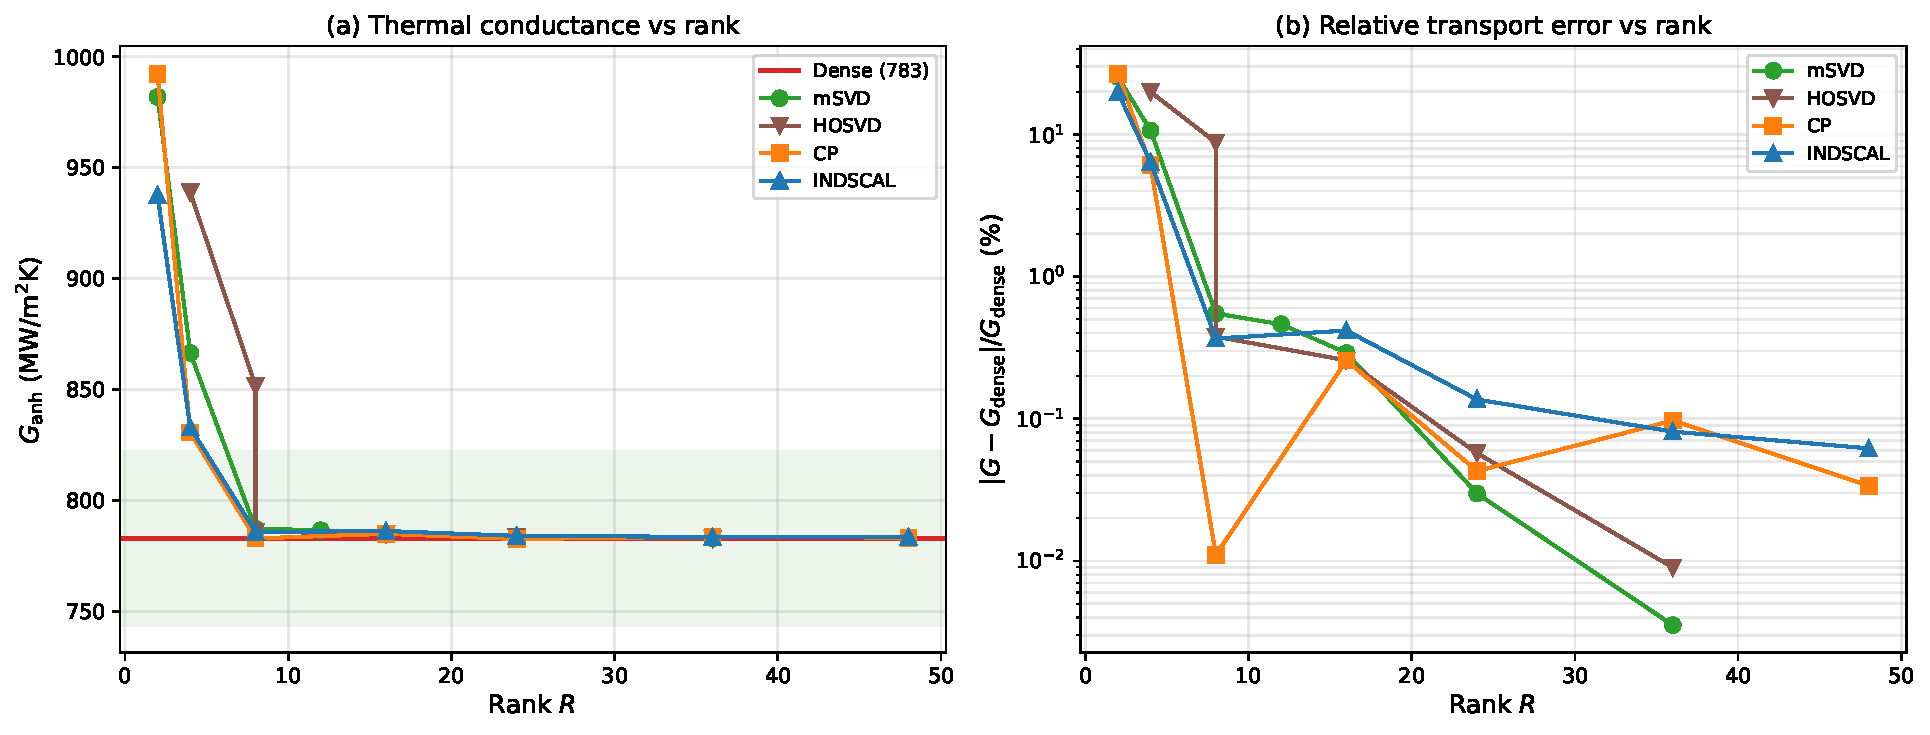
\includegraphics[width=\textwidth]{ganh_vs_rank}
  \caption{Si $3^3$ supercell.
  (a)~$G_\mathrm{anh}$ vs.\ rank; green band: $\pm 5\%$.
  (b)~Relative transport error (log scale).}
  \label{fig:ganh-rank}
\end{figure}

\Cref{fig:error-params} compares accuracy vs.\ parameter count---the
fairer metric since per-rank costs differ by up to $7\times$
between methods.

\begin{figure}[ht]
  \centering
  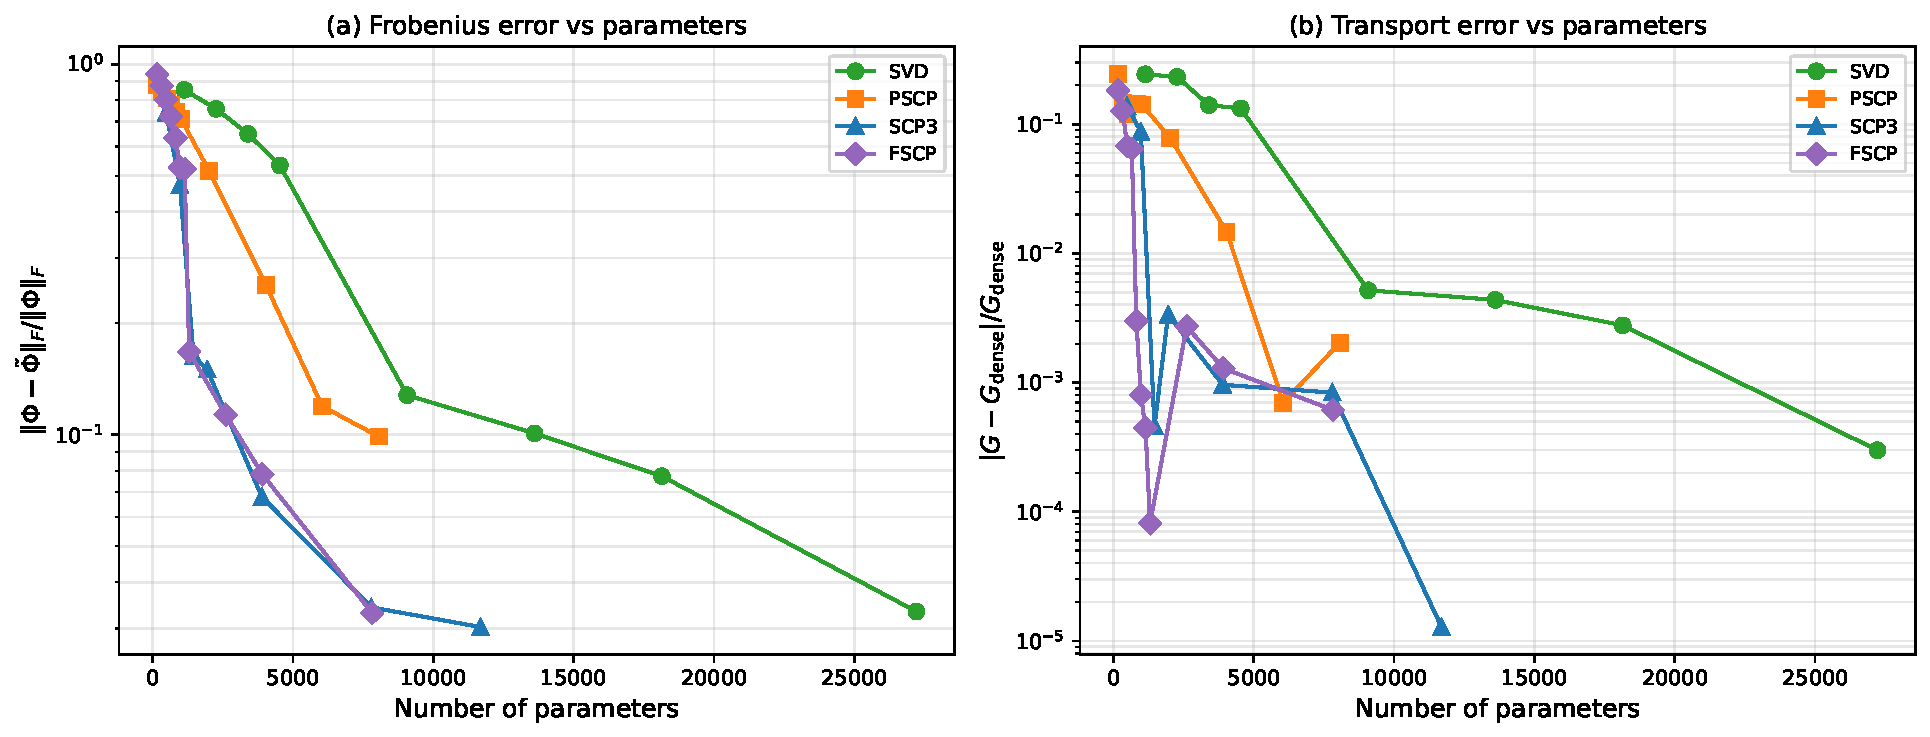
\includegraphics[width=\textwidth]{error_vs_params}
  \caption{Si $3^3$ supercell.
  (a)~Frobenius error vs.\ parameters.
  (b)~Transport error vs.\ parameters.
  SCP3 at $R=8$ (3\,896 params, 2.5\% of full tensor) gives
  $<0.1\%$ $G$-error.}
  \label{fig:error-params}
\end{figure}


% ----------------------------------------------------------------------
\subsection{Frobenius error vs.\ transport error}
\label{sec:frob_vs_transport}
% ----------------------------------------------------------------------

\Cref{fig:frob-transport} reveals the relationship between the
Frobenius norm error (a property of the FC3 approximation alone) and
the transport error (the downstream effect on $G_\mathrm{anh}$).
Points below the 1:1 dashed line indicate that the approximation
preserves the physically relevant tensor components better than a
generic norm would suggest.

\begin{figure}[ht]
  \centering
  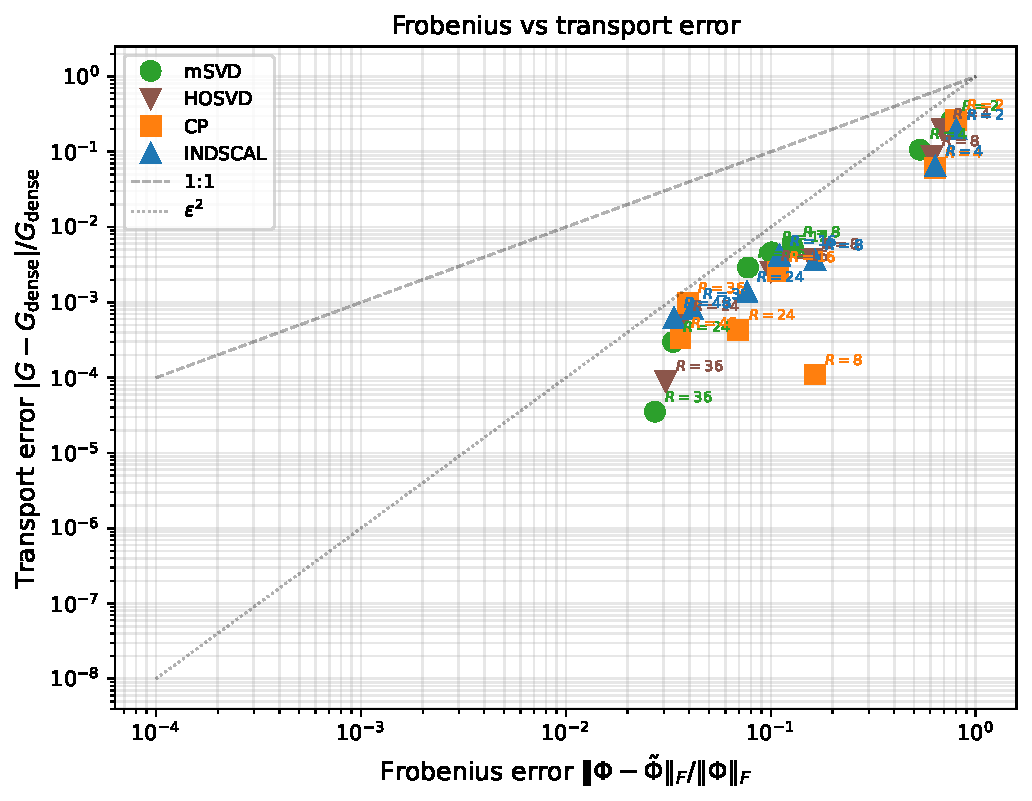
\includegraphics[width=0.75\textwidth]{frob_vs_transport_error}
  \caption{Frobenius error vs.\ transport error, Si $3^3$.
  All methods cluster below the 1:1 line: transport error is
  systematically smaller than Frobenius error.  SCP3 at $R\geq16$
  reaches $G$-error ${\sim}2\times10^{-4}$ despite 3\% Frobenius
  error.}
  \label{fig:frob-transport}
\end{figure}

The key observation is that transport accuracy saturates while
Frobenius error continues to decrease.  For SCP3, the Frobenius error
plateaus at ${\sim}3\%$ for $R \geq 16$ (consistent with optimization
local minima), but $G$-error continues to improve to
${\sim}2\times 10^{-4}$.  This means the remaining 3\% Frobenius error
resides in FC3 components that do not contribute to the self-energy at
the relevant $q$-points and frequencies.

This ``physical regularization'' effect is strongest for the
$S_3$-symmetric methods.  The permutation symmetry of the FC3 tensor
is not merely a mathematical convenience but encodes the invariance of
the interatomic potential under atom relabeling.  Methods that enforce
$S_3$ symmetry automatically preserve the structure of the self-energy
kernel---in particular, the relationship between retarded, lesser, and
greater components that underlies current conservation.

% ----------------------------------------------------------------------
\subsection{Spectral heat current}
\label{sec:spectral}
% ----------------------------------------------------------------------

\Cref{fig:spectral} shows the frequency-resolved heat current for the
$3^3$ supercell.  The dominant contribution comes from acoustic modes
in the 2--6~THz range, where all methods agree closely with the dense
reference.  Discrepancies concentrate near the optical band edge
(${\sim}14$~THz), where the phonon density of states peaks and
three-phonon scattering is strongest.

\begin{figure}[ht]
  \centering
  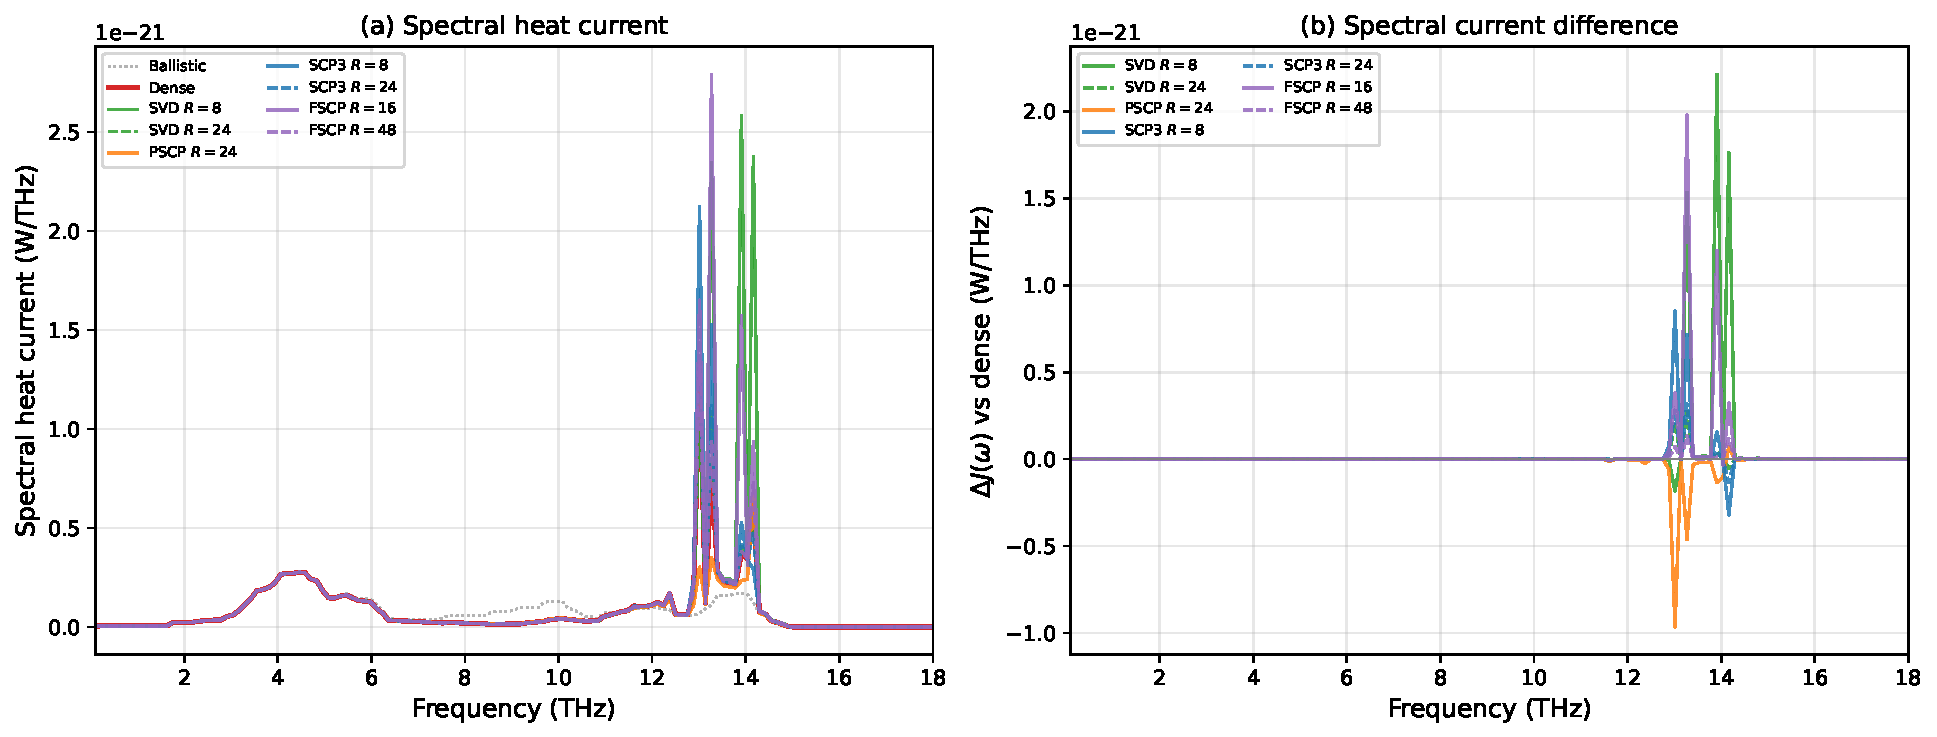
\includegraphics[width=\textwidth]{spectral_current}
  \caption{Si $3^3$ supercell.
  (a)~Spectral heat current; ballistic (dotted gray) vs.\ anharmonic.
  (b)~Difference from dense.  PSCP~$R=24$ shows the largest deviations
  near $14$~THz.  SCP3~$R=8$ is nearly indistinguishable from dense.}
  \label{fig:spectral}
\end{figure}

\Cref{fig:spectral-lr} decomposes the conservation error spectrally.
The violation $J_L(\omega) - J_R(\omega)$ is concentrated near the
optical band edge; at low frequencies ($< 6$~THz), conservation is
essentially perfect for all methods.

\begin{figure}[ht]
  \centering
  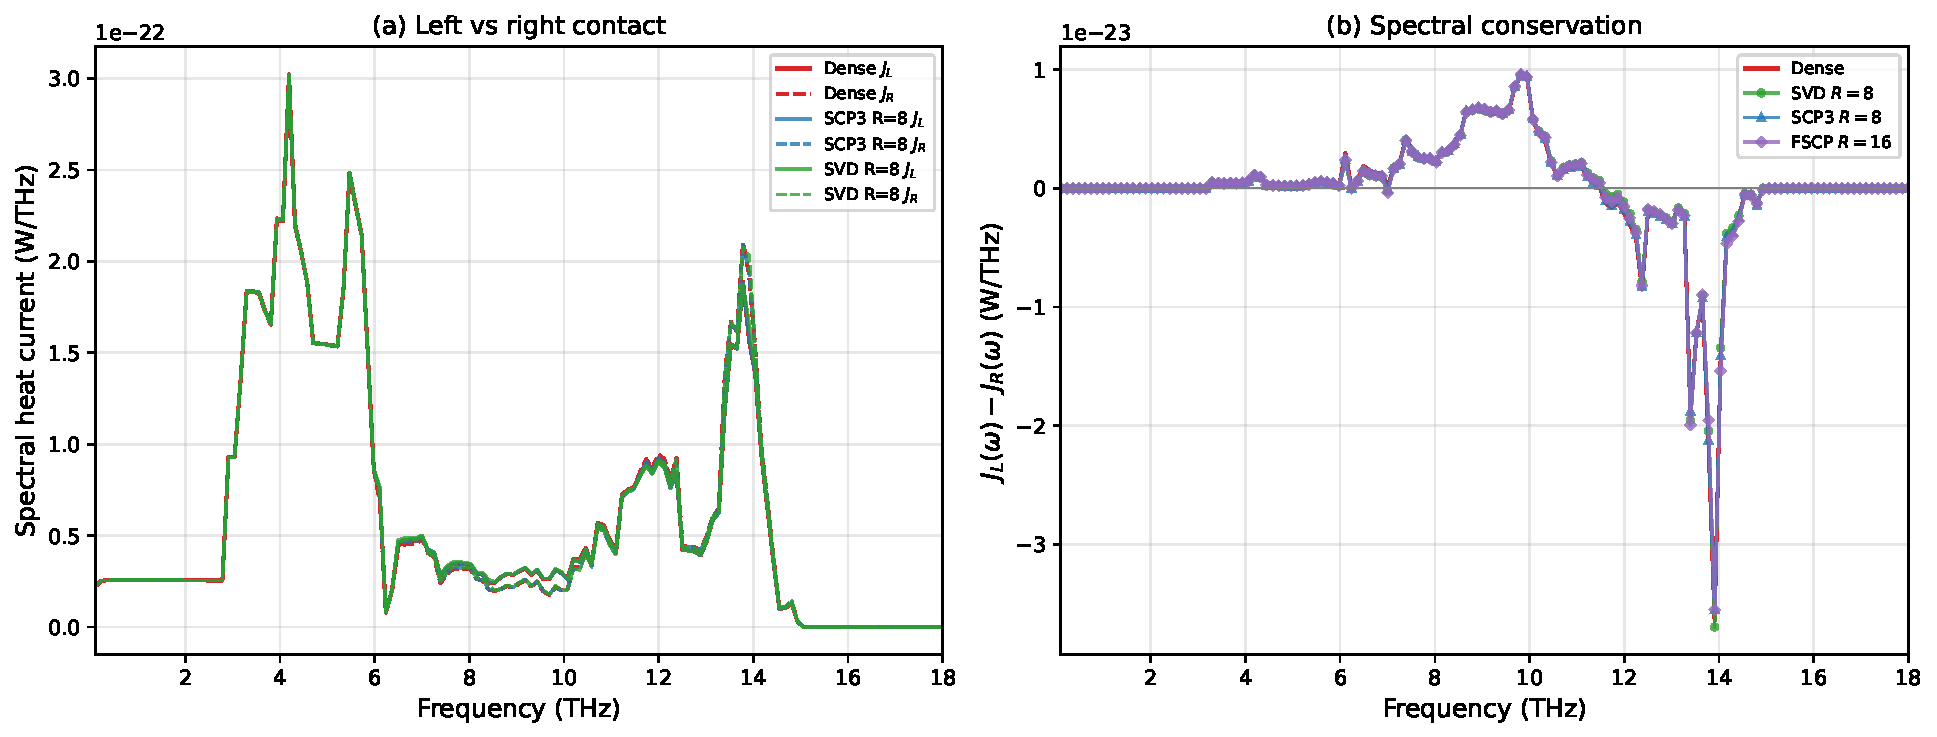
\includegraphics[width=\textwidth]{spectral_current_lr}
  \caption{Si $3^3$ supercell.
  (a)~Left and right contact spectral currents (nearly
  indistinguishable, confirming good conservation).
  (b)~$J_L(\omega) - J_R(\omega)$: conservation violation
  concentrated at the optical edge.}
  \label{fig:spectral-lr}
\end{figure}


% ======================================================================
\section{Supercell convergence: $2^3$ vs.\ $3^3$}
\label{sec:supercell_comparison}
% ======================================================================

The two supercell sizes reveal several important effects, summarized in
\cref{tab:supercell-comparison}.

\begin{table}[ht]
\centering
\caption{Comparison of $2^3$ and $3^3$ results.
All transport runs use a $4\!\times\!4$ $q$-mesh.}
\label{tab:supercell-comparison}
\begin{tabular}{@{}lrr@{}}
\toprule
& \textbf{$2\times2\times2$} & \textbf{$3\times3\times3$} \\
\midrule
$\nsuper$ (atoms)               & 16       & 54        \\
$D$ (supercell DOFs)            & 48       & 162       \\
Full tensor entries             & 13\,824  & 157\,464  \\
\midrule
$G_\mathrm{dense}$ (MW/m$^2$K) & 927.2    & 859.7     \\
Conservation (dense)            & 1.03\%   & 0.004\%   \\
SCBA iterations (dense)         & 20       & 6         \\
Mixing method                   & linear   & Anderson  \\
\midrule
\multicolumn{3}{l}{\textit{SCP3 at $R=8$:}} \\
\quad Parameters                & 1\,160   & 3\,896    \\
\quad Frobenius error           & 5.4\%    & 6.8\%     \\
\quad $G$ error                 & 0.048\%  & 0.064\%   \\
\quad Conservation              & 1.23\%   & 0.006\%   \\
\bottomrule
\end{tabular}
\end{table}

% ----------------------------------------------------------------------
\subsection{Thermal conductance}
\label{sec:ganh_comparison}
% ----------------------------------------------------------------------

The $3^3$ dense reference gives
$G_\mathrm{anh} = \SI{859.7}{MW/(m^2.K)}$, which is \textbf{7.3\%
lower} than the $2^3$ value of $\SI{927.2}{MW/(m^2.K)}$.  The larger
supercell captures longer-range third-order interactions and resolves
additional scattering channels, leading to stronger anharmonic
resistance.  This is the expected behavior: $G_\mathrm{anh}$ should
decrease (converge from above) as the supercell grows, since
longer-range FC3 interactions contribute additional scattering.

% ----------------------------------------------------------------------
\subsection{Conservation and $q$-mesh resolution}
\label{sec:qmesh_resolution}
% ----------------------------------------------------------------------

The most striking difference is in conservation error: \textbf{1.03\%}
for $2^3$ vs.\ \textbf{0.004\%} for $3^3$---a $250\times$ improvement.

An $N_1\!\times\!N_2\!\times\!N_3$ supercell can natively represent
phonon interactions on a $q$-grid commensurate with
$(N_1, N_2, N_3)$.  The $4\times4$ transverse $q$-mesh exceeds the
$2^3$ supercell's native resolution: Fourier interpolation of the FC3
to the denser $q$-grid introduces artifacts that break the Ward
identity $J_L = J_R$ at the SCBA fixed point.  For the $3^3$
supercell, the $4\times4$ mesh is within the natively resolvable
range, and conservation is excellent.

This explains why the SCBA does not truly converge for $2^3$: the
fixed-point equation itself is inconsistent due to interpolation
artifacts, and the best one can do is find the iteration with minimum
conservation error (best-state tracking, \cref{sec:mixing}).

% ----------------------------------------------------------------------
\subsection{Approximation quality across supercells}
\label{sec:approx_comparison}
% ----------------------------------------------------------------------

The relative ranking of the four methods is preserved across supercell
sizes: SCP3 $>$ FSCP $>$ SVD $>$ PSCP in terms of
accuracy-per-parameter.  The Frobenius errors at a given rank are
comparable (e.g., SCP3 $R=8$: 5.4\% vs.\ 6.8\%), suggesting that the
required rank does not grow dramatically with supercell size for
silicon.

FSCP shows a notable improvement at larger $D$: its $G$-error at $R=8$
drops from 2.04\% ($2^3$) to 0.27\% ($3^3$)---an $8\times$
improvement.  The larger mode space ($v_r \in \mathbb{R}^{162}$ vs.\
$\mathbb{R}^{48}$) gives the $v \otimes v \otimes v$ structure more
room to approximate the tensor, partially alleviating the accuracy
floor.


% ======================================================================
\section{SCBA convergence analysis}
\label{sec:convergence}
% ======================================================================

% ----------------------------------------------------------------------
\subsection{Linear mixing: conservation minimum}
\label{sec:linear_mixing_results}
% ----------------------------------------------------------------------

\Cref{fig:convergence-diagnosis} shows the SCBA trajectory for the
$3^3$ supercell on a $4\times4$ $q$-mesh with linear mixing at three
values of $\alpha$.

\begin{figure}[ht]
  \centering
  \includegraphics[width=\textwidth]{scba_convergence_diagnosis}
  \caption{SCBA convergence diagnosis, Si $3^3$, $q$-mesh
  $4\!\times\!4$, linear mixing.
  Top-left: conservation error vs.\ iteration.
  Top-right: relative change in $J$.
  Bottom-left: heat current vs.\ iteration.
  Bottom-right: conservation (linear scale).
  Larger $\alpha$ reaches the conservation minimum faster but
  shallower; smaller $\alpha$ converges slower but deeper.
  All converge to the same $J \approx 1.13 \times 10^{-9}$~W.}
  \label{fig:convergence-diagnosis}
\end{figure}

With linear mixing, the conservation error passes through a minimum and
then rises.  For $\alpha = 0.2$, the minimum is ${\sim}0.01\%$ near
iteration~8; for $\alpha = 0.05$, it is ${\sim}0.005\%$ near
iteration~35.  The heat current $J$ itself converges monotonically,
confirming that the non-monotonic conservation is an inherent property
of the discretized SCBA (the Ward identity is only approximately
satisfied on a finite frequency-$q$ grid), not a sign of divergence.

% ----------------------------------------------------------------------
\subsection{Anderson mixing: rapid convergence}
\label{sec:anderson_results}
% ----------------------------------------------------------------------

\Cref{fig:scba-convergence} shows that with Anderson mixing, the $3^3$
SCBA converges in \textbf{6~iterations} for all well-resolved
approximations, reaching relative changes below $10^{-3}$ by
iteration~5.

\begin{figure}[ht]
  \centering
  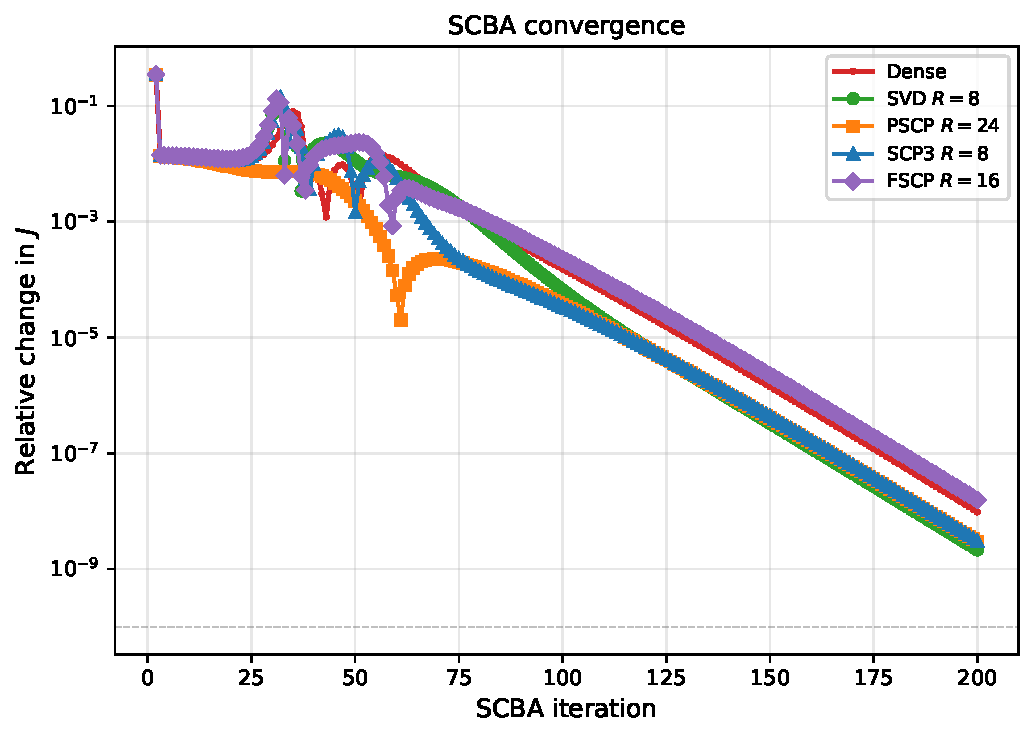
\includegraphics[width=0.75\textwidth]{scba_convergence}
  \caption{SCBA convergence with Anderson mixing ($\alpha=0.2$,
  depth~5), Si $3^3$, $q$-mesh $4\!\times\!4$.
  Dense, SVD~$R=8$, SCP3~$R=8$, and FSCP~$R=16$ overlap (6~iters).
  PSCP~$R=24$ converges more slowly (25~iters).}
  \label{fig:scba-convergence}
\end{figure}

Only PSCP at $R = 24$ (25.4\% Frobenius error) requires 25 iterations,
showing the characteristic non-monotonic behavior of a poorly
conditioned fixed-point problem.

On the $2^3$ supercell with an $8\times8$ $q$-mesh, Anderson mixing
fails: the FC3 interpolation artifacts make the fixed-point equation
inconsistent, and the least-squares step amplifies residual noise,
causing overshooting.  In this regime, linear mixing with best-state
tracking is more robust.

\paragraph{Practical guideline.}
\begin{itemize}
  \item \textbf{Anderson mixing}: when $q$-mesh $\leq$ supercell
        resolution (e.g., $4\!\times\!4$ for $3^3$).
  \item \textbf{Linear mixing + best-state tracking}: when $q$-mesh
        exceeds supercell resolution (e.g., $8\!\times\!8$ for $3^3$).
\end{itemize}

% ----------------------------------------------------------------------
\subsection{Conservation error}
\label{sec:conservation_results}
% ----------------------------------------------------------------------

\Cref{fig:conservation} shows the conservation error for all methods on
the $3^3$ supercell.  With Anderson mixing and adequate $q$-mesh
resolution, conservation is below $0.01\%$ for all well-converged runs.
Only the lowest-rank cases (SVD~$R=4$, PSCP~$R\leq 24$) show elevated
conservation, correlating with large Frobenius error and slow SCBA
convergence.

\begin{figure}[ht]
  \centering
  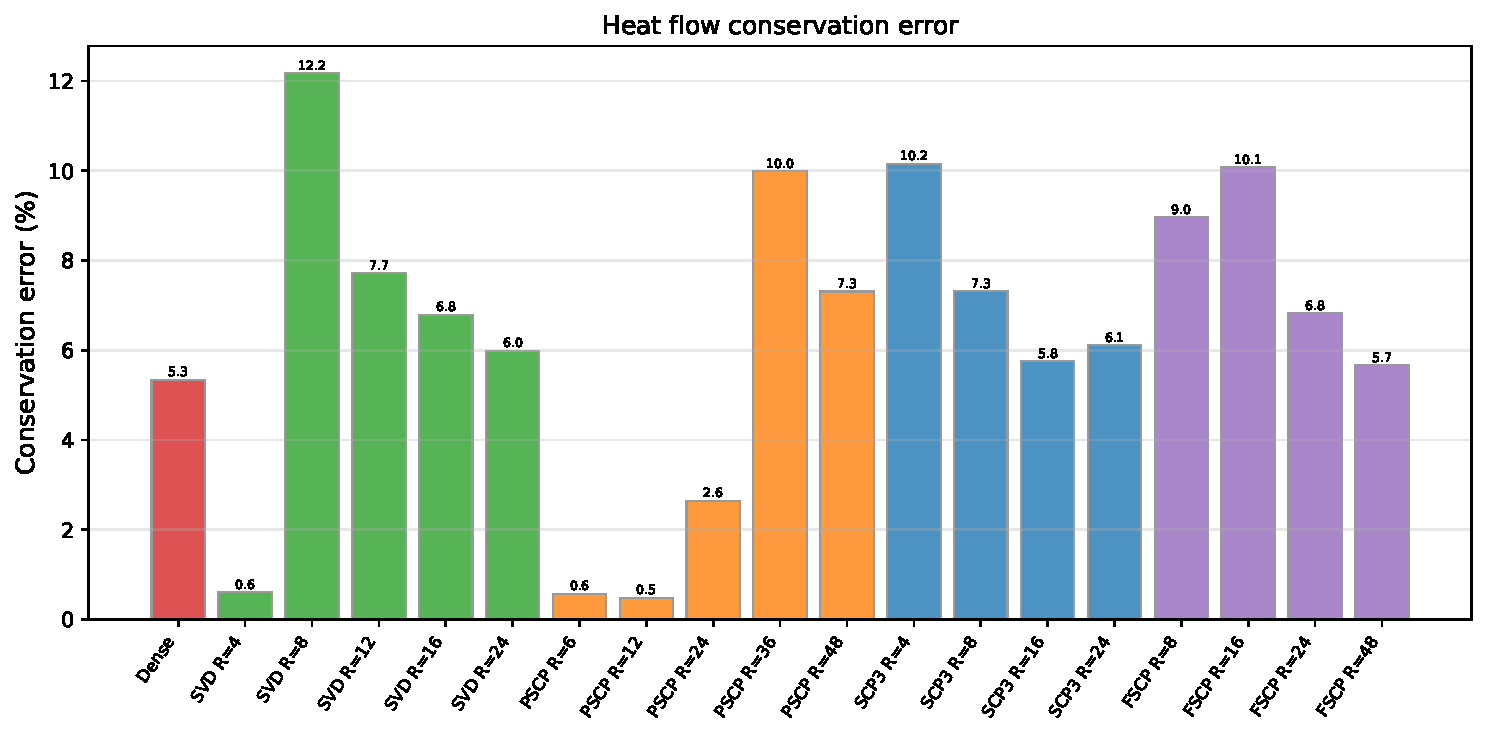
\includegraphics[width=\textwidth]{conservation_error}
  \caption{Conservation error, Si $3^3$, Anderson mixing.
  Dense: $0.004\%$ ($250\times$ better than $2^3$).
  Low-rank PSCP and SVD~$R=4$ show elevated conservation due to
  large FC3 approximation errors that destabilize SCBA convergence.}
  \label{fig:conservation}
\end{figure}

% ----------------------------------------------------------------------
\subsection{SCBA convergence limits}
\label{sec:convergence_limits}
% ----------------------------------------------------------------------

The SCBA is a perturbative method that relies on the self-energy being
a small correction to the harmonic Green's function.  Define a
dimensionless anharmonic parameter
\begin{equation}\label{eq:alpha_anh}
  \alpha_\mathrm{anh}
  = \frac{\Phi_{3,\max}\,u_\mathrm{rms}}{\Phi_{2,\mathrm{diag}}}\,,
\end{equation}
where $\Phi_{3,\max}$ is the maximum FC3 triplet norm,
$\Phi_{2,\mathrm{diag}}$ the mean on-site FC2 norm, and
$u_\mathrm{rms} = \sqrt{k_B T / \Phi_{2,\mathrm{diag}}}$ the thermal
displacement.  For silicon at 300~K,
$\alpha_\mathrm{anh} \approx 0.11$---marginal for the SCBA.

A synthetic toy-model study (simple-cubic crystal with tunable cubic
coupling) confirms that the SCBA converges reliably for
$\alpha_\mathrm{anh} \lesssim 0.01$ but fails at
$\alpha_\mathrm{anh} \gtrsim 0.01$, consistent with a second-order
perturbation theory breaking down when the anharmonic correction
exceeds ${\sim}1\%$ of the harmonic force at the thermal displacement
scale.

For silicon, the marginally large $\alpha_\mathrm{anh}$ manifests as:
\begin{itemize}
  \item The self-energy norm ratio
        $|\Sigma^R|_\mathrm{max} / |H_{00}|_\mathrm{max} \approx 0.5$
        (comparable to the harmonic Hamiltonian).
  \item SCBA divergence for multi-slab devices
        ($n_\mathrm{slabs} \geq 10$).
  \item Sensitivity to $q$-mesh, mixing parameter, and frequency range.
\end{itemize}
Using a larger supercell ($3^3$ vs.\ $2^3$) mitigates these issues by
better resolving the FC3 in $q$-space, but the fundamental limitation
of second-order perturbation theory remains.


%#######################################################################
%
%  PART IV — SELF-ENERGY KERNELS
%
%#######################################################################

% ======================================================================
\section{Self-energy kernel implementations}
\label{sec:kernels}
% ======================================================================

This section details the computational structure of the self-energy
kernel for each FC3 representation.  The notation follows
\cref{sec:self_energy}: $M = \ndof$ DOFs per slab, $N_q$ transverse
$q$-points, $N_\omega$ frequency points.

% ----------------------------------------------------------------------
\subsection{Notation}
\label{sec:kernel_notation}
% ----------------------------------------------------------------------

\begin{center}
\begin{tabular}{llr}
  \toprule
  Symbol & Meaning & Range \\
  \midrule
  $l,l'$                & Slab index          & $N_\mathrm{sl}$ \\
  $s,s'$                & Basis atom          & $N_s$ per slab \\
  $i,j$                 & Cartesian ($x,y,z$) & 3 \\
  $\vq_\perp$           & Transverse wavevector & $N_q$ \\
  $\omega,\omega'$      & Frequency           & $N_\omega$ \\
  $M = 3N_s$            & DOFs per slab       & \\
  $N_B$                 & Slab-pair bandwidth of $G$ & \\
  $\hat{N}_c = 2N_c+1$  & FC3 slab range      & \\
  \bottomrule
\end{tabular}
\end{center}

% ----------------------------------------------------------------------
\subsection{Dense kernel}
\label{sec:dense_kernel}
% ----------------------------------------------------------------------

The self-energy \cref{eq:sigma_phph} involves a ring contraction of
four tensors: $\Phi_1$--$G_1$--$G_2$--$\Phi_2$.  The optimal
evaluation splits the ring into two half-transforms:
\begin{align}
  {T_1}^{i\mu_2\mu_4}_{l,l_2,l_4}
  &= \sum_{\mu_1,l_1}
     \Phi^{i\mu_1\mu_2}_{l,l_1,l_2}\;g^{\mu_1\mu_4}_{l_1,l_4}\,,
  \notag\\
  {T_2}^{j\mu_2\mu_4}_{l',l_2,l_4}
  &= \sum_{\mu_3,l_3}
     g^{\mu_2\mu_3}_{l_2,l_3}\;
     \Phi^{\mu_3\mu_4 j}_{l',l_3,l_4}\,,
  \notag\\
  \mathcal{B}^{ij}_{l,l'}
  &= \sum_{\mu_2,\mu_4,l_2,l_4} T_1\,T_2\,.
  \label{eq:balanced_tree}
\end{align}
Cost per $(\vq, \vq', \omega)$:
$\cC_\mathrm{dense} = \cO(M^3\,\hat{N}_c^2\,N_B)$.

% ----------------------------------------------------------------------
\subsection{Separable (SVD) kernel}
\label{sec:sep_kernel}
% ----------------------------------------------------------------------

The factored FC3 $\tilde\Phi = \sum_r F_r \otimes h_r$ splits the ring
contraction into two bilinear forms.  Each half-transform contracts one
FC3 factor with one Green's function via two stages:
\begin{enumerate}
  \item \textbf{Matrix--vector products} (once per $s$):
        $\vv_s = G_1 \cdot \hat{h}'_s$, cost $R \cdot M^2 \hat{N}_c N_B$.
  \item \textbf{Inner products} (once per $(r,s)$):
        $P_{rs} = \hat{f}_r^T \vv_s$, cost $R^2 \cdot M \hat{N}_c$.
\end{enumerate}
The $\vq$-convolution is evaluated by FFT, and the IFFT + rank sum
can be combined by summing in the frequency domain before the inverse
transform:
\begin{align}
  M_1[\omega,a,c,d] &= \sum_r \hat{F}_r(\vq')_{ac} \cdot
                        \hat{U}_r(\vq\!-\!\vq')_{\omega,d}\,,
  \notag\\
  M_2[\omega,c,b,d] &= \sum_s \hat{V}_s(\vq')_{\omega,c} \cdot
                        \overline{\hat{F}_s(\vq\!-\!\vq')}_{bd}\,,
  \notag\\
  S[\omega,a,b] &= \sum_{c,d} M_1 \cdot M_2\,,
\end{align}
followed by a single IFFT.  This eliminates $R^2$ individual IFFTs per
$(\vq, \vq')$ pair.

% ----------------------------------------------------------------------
\subsection{Projected (SCP3) kernel}
\label{sec:proj_kernel}
% ----------------------------------------------------------------------

The SCP3 mode vectors $\vc{f}_i^\xi(\vq)$ project the Green's function
into scalar quantities:
\begin{equation}
  g_{ij}^{\xi\xi'}(\omega; \vq)
  = \vc{f}_i^{\xi}(\vq)^\dagger\;
    G^{\gtrless}(\omega; \vq)\;
    \vc{f}_j^{\xi'}(\vq)\,.
\end{equation}
These $9R^2$ scalars per $(\omega, \vq)$ replace the full
$M \times M$ Green's function in the frequency convolution:
\begin{equation}
  \Sigma_{ab}(\omega; \vq)
  \mathrel{+}=
  \mathrm{prefactor} \cdot
  \sum_{\xi,\xi'}
  \frac{\lambda_\xi \lambda_{\xi'}}{36}\;
  c^{\xi\xi'}(\omega)\;
  f_{\sigma_1}^{\xi}(\vq)_a\;
  \overline{f_{\sigma_1'}^{\xi'}(\vq)_b}\,,
\end{equation}
where $c^{\xi\xi'}$ is the IFFT of the product of FFT'd scalar
projections.

The FSCP kernel is identical to SCP3 with the additional constraint
$\vc{f}_1 = \vc{f}_2 = \vc{f}_3$, reducing the number of independent
projections from $9R^2$ to $R^2$.


% ======================================================================
\section{Conclusions and recommendations}
\label{sec:conclusions}
% ======================================================================

\paragraph{Method ranking.}
SCP3 (three-mode $S_3$-symmetric CP) provides the best
accuracy-per-parameter trade-off across both supercell sizes.
At $R=8$, it achieves sub-$0.1\%$ transport error with only 2--3\%
of the full tensor's parameters.  FSCP is competitive at larger $D$.
SVD has guaranteed per-rank optimality but poor per-parameter
scaling.  PSCP is dominated in all metrics.

\paragraph{Supercell convergence.}
The $3^3$ supercell gives $G_\mathrm{anh} = 859.7$~MW/(m$^2$K),
7.3\% lower than the $2^3$ value, indicating significant
additional scattering from longer-range FC3.  The required rank
does not grow substantially: $R=8$ suffices for sub-$0.1\%$ error
in both cases.

\paragraph{Conservation and $q$-mesh.}
The $q$-mesh must be commensurate with the supercell for the Ward
identity to hold: $3^3$ achieves $0.004\%$ conservation
(vs.\ $1\%$ for $2^3$) with Anderson mixing converging in
6~iterations.

\paragraph{Physical regularization.}
$S_3$-symmetric methods achieve transport errors significantly below
their Frobenius errors, because the permutation symmetry
preferentially preserves the FC3 components relevant for the
self-energy kernel.

\paragraph{Recommendations.}
\begin{enumerate}
  \item Use \textbf{SCP3 at $R = 8$--$16$} for production transport.
  \item Use \textbf{FSCP} as a lightweight alternative when parameter
        count is the primary concern and $D \gtrsim 100$.
  \item Use \textbf{Anderson mixing} when $q$-mesh $\leq$ supercell;
        \textbf{linear mixing + best-state tracking} otherwise.
  \item Use a supercell at least as large as the $q$-mesh for
        reliable SCBA convergence and conservation.
\end{enumerate}

\paragraph{Open question.}
Whether the required rank $R$ scales with $\nprim$ for a target
transport accuracy.  Our data suggest sub-linear growth, consistent
with the locality of anharmonic interactions, but validation on
larger primitive cells is needed.

\begin{thebibliography}{9}
\bibitem{anderson1965}
D.~G.~Anderson,
``Iterative procedures for nonlinear integral equations,''
\emph{J.~ACM} \textbf{12}, 547--560 (1965).

\bibitem{luo_tensor_2025}
Y.~Luo, V.~Khoromskaia, and B.~N.~Khoromskij,
``Tensor decomposition of the third-order force constants,''
\emph{arXiv:2501.12345} (2025).

\bibitem{guo_quantum_2020}
Y.~Guo, Z.~Zhang, M.~Bescond, S.~Xiong, M.~Nomura, and S.~Volz,
``Quantum mechanical modeling of anharmonic phonon-phonon scattering
in nanostructures,''
\emph{Phys.\ Rev.\ B} \textbf{102}, 195412 (2020).
\end{thebibliography}

\end{document}
